\pdfoutput=1
\documentclass{article}

\usepackage{amsmath, amsthm, amssymb}
\usepackage{natbib}
\usepackage{booktabs}
\usepackage{graphicx}
\usepackage{hyperref}
\usepackage[margin=1.4in]{geometry}
\hypersetup{colorlinks,citecolor=blue,urlcolor=blue,linkcolor=blue,
  pdftitle={Higher-Order Asymptotics of Regression-Adjusted Estimators in Randomized Trials},
  pdfauthor={Anna Kelley and Stefan Wager}}
\setlength{\emergencystretch}{3em}

%%%%%%%%% Macros (self-contained: this file compiles without any local .sty)
\newcommand{\RR}{\mathbb{R}}
\newcommand{\nn}{\mathcal{N}}
\newcommand{\EEE}{\mathbb{E}}
\newcommand{\EE}[1]{\mathbb{E}\left[#1\right]}
\newcommand{\Var}[1]{\operatorname{Var}\left[#1\right]}
\newcommand{\PP}[1]{\mathbb{P}\left[#1\right]}
\newcommand{\p}[1]{\left(#1\right)}
\newcommand{\cb}[1]{\left\{#1\right\}}
\newcommand{\abs}[1]{\left|#1\right|}
\newcommand{\cond}{\;\middle|\;}
\newcommand{\htau}{\hat{\tau}}
\newcommand{\hdelta}{\hat{\delta}}
\newcommand{\hbeta}{\hat{\beta}}
\DeclareMathOperator*{\argmin}{argmin}
\newcommand{\limn}{\lim_{n\to\infty}}
\DeclareMathOperator{\MSE}{MSE}
\DeclareMathOperator{\tr}{tr}
\DeclareMathOperator{\Cov}{Cov}
\newcommand{\Bern}{\mathrm{Bern}}
\newcommand{\CRT}{\mathrm{CRT}}
\newcommand{\IREG}{\mathrm{IREG}}
\newcommand{\REG}{\mathrm{REG}}
\newcommand{\SATE}{\mathrm{SATE}}
\newcommand{\MSEexp}{\MSE^{\mathrm{exp}}}
% numbers quoted in the prose of Section 3 and Appendix D are generated from results/*.json
% generated by simulations/make_tables.py from results/*.json -- do not edit
\expandafter\def\csname gz:all:REG_HC1:max\endcsname{95.4}
\expandafter\def\csname gz:all:REG_HC1:min\endcsname{94.7}
\expandafter\def\csname gz:analytic:cov:0.01\endcsname{94.9}
\expandafter\def\csname gz:analytic:cov:0.1\endcsname{93.7}
\expandafter\def\csname gz:bias:gauss:maxrelerr\endcsname{0.8}
\expandafter\def\csname gz:bias:gauss:ndesigns\endcsname{5}
\expandafter\def\csname gz:corr:heavy_tail_example:IREG_HC1:0.80\endcsname{67.2}
\expandafter\def\csname gz:corr:heavy_tail_example:IREG_HC1:0.90\endcsname{78.5}
\expandafter\def\csname gz:corr:heavy_tail_example:IREG_HC1:0.95\endcsname{85.6}
\expandafter\def\csname gz:corr:heavy_tail_example:IREG_HC1:0.98\endcsname{91.2}
\expandafter\def\csname gz:corr:heavy_tail_example:IREG_HC1:0.99\endcsname{93.7}
\expandafter\def\csname gz:corr:heavy_tail_example:IREG_HC1c:0.80\endcsname{75.3}
\expandafter\def\csname gz:corr:heavy_tail_example:IREG_HC1c:0.90\endcsname{88.1}
\expandafter\def\csname gz:corr:heavy_tail_example:IREG_HC1c:0.95\endcsname{94.4}
\expandafter\def\csname gz:corr:heavy_tail_example:IREG_HC1c:0.98\endcsname{97.9}
\expandafter\def\csname gz:corr:heavy_tail_example:IREG_HC1c:0.99\endcsname{99.1}
\expandafter\def\csname gz:corr:heavy_tail_example:IREG_HC1o:0.80\endcsname{68.2}
\expandafter\def\csname gz:corr:heavy_tail_example:IREG_HC1o:0.90\endcsname{79.5}
\expandafter\def\csname gz:corr:heavy_tail_example:IREG_HC1o:0.95\endcsname{86.5}
\expandafter\def\csname gz:corr:heavy_tail_example:IREG_HC1o:0.98\endcsname{91.8}
\expandafter\def\csname gz:corr:heavy_tail_example:IREG_HC1o:0.99\endcsname{94.2}
\expandafter\def\csname gz:corr:heavy_tail_example:IREG_HC3:0.80\endcsname{79.8}
\expandafter\def\csname gz:corr:heavy_tail_example:IREG_HC3:0.90\endcsname{89.3}
\expandafter\def\csname gz:corr:heavy_tail_example:IREG_HC3:0.95\endcsname{94.0}
\expandafter\def\csname gz:corr:heavy_tail_example:IREG_HC3:0.98\endcsname{97.0}
\expandafter\def\csname gz:corr:heavy_tail_example:IREG_HC3:0.99\endcsname{98.2}
\expandafter\def\csname gz:corr:heavy_tail_example:IREG_HC3c:0.80\endcsname{84.9}
\expandafter\def\csname gz:corr:heavy_tail_example:IREG_HC3c:0.90\endcsname{93.6}
\expandafter\def\csname gz:corr:heavy_tail_example:IREG_HC3c:0.95\endcsname{97.3}
\expandafter\def\csname gz:corr:heavy_tail_example:IREG_HC3c:0.98\endcsname{99.1}
\expandafter\def\csname gz:corr:heavy_tail_example:IREG_HC3c:0.99\endcsname{99.6}
\expandafter\def\csname gz:corr:heavy_tail_example:R2\endcsname{0.009}
\expandafter\def\csname gz:corr:heavy_tail_example:REG_HC1:0.80\endcsname{76.2}
\expandafter\def\csname gz:corr:heavy_tail_example:REG_HC1:0.90\endcsname{88.3}
\expandafter\def\csname gz:corr:heavy_tail_example:REG_HC1:0.95\endcsname{94.4}
\expandafter\def\csname gz:corr:heavy_tail_example:REG_HC1:0.98\endcsname{97.8}
\expandafter\def\csname gz:corr:heavy_tail_example:REG_HC1:0.99\endcsname{99.0}
\expandafter\def\csname gz:corr:heavy_tail_example:ratio\endcsname{31}
\expandafter\def\csname gz:corr:heavy_tail_example:reps\endcsname{100{,}000}
\expandafter\def\csname gz:corr:heavy_tail_example:wr\endcsname{1.06}
\expandafter\def\csname gz:corr:heavy_tail_example:wr_cover\endcsname{1.04}
\expandafter\def\csname gz:corr:heavy_tail_example:wr_miss\endcsname{1.35}
\expandafter\def\csname gz:corr:large_hte_n500_p5:Delta\endcsname{4.2}
\expandafter\def\csname gz:corr:large_hte_n500_p5:IREG_HC1:0.80\endcsname{52.1}
\expandafter\def\csname gz:corr:large_hte_n500_p5:IREG_HC1:0.90\endcsname{63.9}
\expandafter\def\csname gz:corr:large_hte_n500_p5:IREG_HC1:0.95\endcsname{72.7}
\expandafter\def\csname gz:corr:large_hte_n500_p5:IREG_HC1:0.98\endcsname{80.7}
\expandafter\def\csname gz:corr:large_hte_n500_p5:IREG_HC1:0.99\endcsname{85.3}
\expandafter\def\csname gz:corr:large_hte_n500_p5:IREG_HC1c:0.80\endcsname{80.2}
\expandafter\def\csname gz:corr:large_hte_n500_p5:IREG_HC1c:0.90\endcsname{90.0}
\expandafter\def\csname gz:corr:large_hte_n500_p5:IREG_HC1c:0.95\endcsname{95.2}
\expandafter\def\csname gz:corr:large_hte_n500_p5:IREG_HC1c:0.98\endcsname{98.1}
\expandafter\def\csname gz:corr:large_hte_n500_p5:IREG_HC1c:0.99\endcsname{99.1}
\expandafter\def\csname gz:corr:large_hte_n500_p5:IREG_HC1o:0.80\endcsname{80.2}
\expandafter\def\csname gz:corr:large_hte_n500_p5:IREG_HC1o:0.90\endcsname{90.0}
\expandafter\def\csname gz:corr:large_hte_n500_p5:IREG_HC1o:0.95\endcsname{95.1}
\expandafter\def\csname gz:corr:large_hte_n500_p5:IREG_HC1o:0.98\endcsname{98.2}
\expandafter\def\csname gz:corr:large_hte_n500_p5:IREG_HC1o:0.99\endcsname{99.2}
\expandafter\def\csname gz:corr:large_hte_n500_p5:IREG_HC3:0.80\endcsname{52.7}
\expandafter\def\csname gz:corr:large_hte_n500_p5:IREG_HC3:0.90\endcsname{64.6}
\expandafter\def\csname gz:corr:large_hte_n500_p5:IREG_HC3:0.95\endcsname{73.3}
\expandafter\def\csname gz:corr:large_hte_n500_p5:IREG_HC3:0.98\endcsname{81.3}
\expandafter\def\csname gz:corr:large_hte_n500_p5:IREG_HC3:0.99\endcsname{85.7}
\expandafter\def\csname gz:corr:large_hte_n500_p5:IREG_HC3c:0.80\endcsname{80.4}
\expandafter\def\csname gz:corr:large_hte_n500_p5:IREG_HC3c:0.90\endcsname{90.1}
\expandafter\def\csname gz:corr:large_hte_n500_p5:IREG_HC3c:0.95\endcsname{95.3}
\expandafter\def\csname gz:corr:large_hte_n500_p5:IREG_HC3c:0.98\endcsname{98.2}
\expandafter\def\csname gz:corr:large_hte_n500_p5:IREG_HC3c:0.99\endcsname{99.1}
\expandafter\def\csname gz:corr:large_hte_n500_p5:R2\endcsname{0.692}
\expandafter\def\csname gz:corr:large_hte_n500_p5:REG_HC1:0.80\endcsname{80.2}
\expandafter\def\csname gz:corr:large_hte_n500_p5:REG_HC1:0.90\endcsname{90.2}
\expandafter\def\csname gz:corr:large_hte_n500_p5:REG_HC1:0.95\endcsname{95.2}
\expandafter\def\csname gz:corr:large_hte_n500_p5:REG_HC1:0.98\endcsname{98.2}
\expandafter\def\csname gz:corr:large_hte_n500_p5:REG_HC1:0.99\endcsname{99.1}
\expandafter\def\csname gz:corr:large_hte_n500_p5:ratio\endcsname{1.00}
\expandafter\def\csname gz:corr:large_hte_n500_p5:reps\endcsname{20{,}000}
\expandafter\def\csname gz:corr:large_hte_n500_p5:wr\endcsname{1.80}
\expandafter\def\csname gz:corr:large_hte_n500_p5:wr_cover\endcsname{1.80}
\expandafter\def\csname gz:corr:large_hte_n500_p5:wr_miss\endcsname{1.80}
\expandafter\def\csname gz:corr:lognormal_s2.0_prop:IREG_HC1:0.80\endcsname{64.4}
\expandafter\def\csname gz:corr:lognormal_s2.0_prop:IREG_HC1:0.90\endcsname{75.5}
\expandafter\def\csname gz:corr:lognormal_s2.0_prop:IREG_HC1:0.95\endcsname{83.0}
\expandafter\def\csname gz:corr:lognormal_s2.0_prop:IREG_HC1:0.98\endcsname{89.1}
\expandafter\def\csname gz:corr:lognormal_s2.0_prop:IREG_HC1:0.99\endcsname{91.9}
\expandafter\def\csname gz:corr:lognormal_s2.0_prop:IREG_HC1c:0.80\endcsname{74.6}
\expandafter\def\csname gz:corr:lognormal_s2.0_prop:IREG_HC1c:0.90\endcsname{88.3}
\expandafter\def\csname gz:corr:lognormal_s2.0_prop:IREG_HC1c:0.95\endcsname{95.1}
\expandafter\def\csname gz:corr:lognormal_s2.0_prop:IREG_HC1c:0.98\endcsname{98.6}
\expandafter\def\csname gz:corr:lognormal_s2.0_prop:IREG_HC1c:0.99\endcsname{99.5}
\expandafter\def\csname gz:corr:lognormal_s2.0_prop:IREG_HC1o:0.80\endcsname{64.4}
\expandafter\def\csname gz:corr:lognormal_s2.0_prop:IREG_HC1o:0.90\endcsname{75.5}
\expandafter\def\csname gz:corr:lognormal_s2.0_prop:IREG_HC1o:0.95\endcsname{83.0}
\expandafter\def\csname gz:corr:lognormal_s2.0_prop:IREG_HC1o:0.98\endcsname{89.1}
\expandafter\def\csname gz:corr:lognormal_s2.0_prop:IREG_HC1o:0.99\endcsname{91.9}
\expandafter\def\csname gz:corr:lognormal_s2.0_prop:IREG_HC3:0.80\endcsname{79.5}
\expandafter\def\csname gz:corr:lognormal_s2.0_prop:IREG_HC3:0.90\endcsname{89.2}
\expandafter\def\csname gz:corr:lognormal_s2.0_prop:IREG_HC3:0.95\endcsname{93.9}
\expandafter\def\csname gz:corr:lognormal_s2.0_prop:IREG_HC3:0.98\endcsname{96.9}
\expandafter\def\csname gz:corr:lognormal_s2.0_prop:IREG_HC3:0.99\endcsname{98.0}
\expandafter\def\csname gz:corr:lognormal_s2.0_prop:IREG_HC3c:0.80\endcsname{85.7}
\expandafter\def\csname gz:corr:lognormal_s2.0_prop:IREG_HC3c:0.90\endcsname{94.6}
\expandafter\def\csname gz:corr:lognormal_s2.0_prop:IREG_HC3c:0.95\endcsname{98.1}
\expandafter\def\csname gz:corr:lognormal_s2.0_prop:IREG_HC3c:0.98\endcsname{99.5}
\expandafter\def\csname gz:corr:lognormal_s2.0_prop:IREG_HC3c:0.99\endcsname{99.8}
\expandafter\def\csname gz:corr:lognormal_s2.0_prop:R2\endcsname{0.000}
\expandafter\def\csname gz:corr:lognormal_s2.0_prop:REG_HC1:0.80\endcsname{76.3}
\expandafter\def\csname gz:corr:lognormal_s2.0_prop:REG_HC1:0.90\endcsname{88.8}
\expandafter\def\csname gz:corr:lognormal_s2.0_prop:REG_HC1:0.95\endcsname{95.3}
\expandafter\def\csname gz:corr:lognormal_s2.0_prop:REG_HC1:0.98\endcsname{98.6}
\expandafter\def\csname gz:corr:lognormal_s2.0_prop:REG_HC1:0.99\endcsname{99.5}
\expandafter\def\csname gz:corr:lognormal_s2.0_prop:ratio\endcsname{--}
\expandafter\def\csname gz:corr:lognormal_s2.0_prop:reps\endcsname{20{,}000}
\expandafter\def\csname gz:corr:lognormal_s2.0_prop:wr\endcsname{1.07}
\expandafter\def\csname gz:corr:lognormal_s2.0_prop:wr_cover\endcsname{1.05}
\expandafter\def\csname gz:corr:lognormal_s2.0_prop:wr_miss\endcsname{1.48}
\expandafter\def\csname gz:corr:mcse:max\endcsname{0.4}
\expandafter\def\csname gz:def:s0.8\endcsname{12}
\expandafter\def\csname gz:def:s1.0\endcsname{41}
\expandafter\def\csname gz:def:s1.2\endcsname{166}
\expandafter\def\csname gz:defpred:s0.8:n2000\endcsname{0.6}
\expandafter\def\csname gz:defpred:s0.8:n500\endcsname{2.4}
\expandafter\def\csname gz:defpred:s0.8:n8000\endcsname{0.2}
\expandafter\def\csname gz:defpred:s1.0:n2000\endcsname{2.1}
\expandafter\def\csname gz:defpred:s1.0:n500\endcsname{8.3}
\expandafter\def\csname gz:defpred:s1.0:n8000\endcsname{0.5}
\expandafter\def\csname gz:defpred:s1.2:n2000\endcsname{8.3}
\expandafter\def\csname gz:defpred:s1.2:n500\endcsname{33.2}
\expandafter\def\csname gz:defpred:s1.2:n8000\endcsname{2.1}
\expandafter\def\csname gz:defsim:s0.8:n2000\endcsname{0.5}
\expandafter\def\csname gz:defsim:s0.8:n500\endcsname{1.8}
\expandafter\def\csname gz:defsim:s0.8:n8000\endcsname{0.1}
\expandafter\def\csname gz:defsim:s1.0:n2000\endcsname{1.4}
\expandafter\def\csname gz:defsim:s1.0:n500\endcsname{4.3}
\expandafter\def\csname gz:defsim:s1.0:n8000\endcsname{0.4}
\expandafter\def\csname gz:defsim:s1.2:n2000\endcsname{3.5}
\expandafter\def\csname gz:defsim:s1.2:n500\endcsname{9.2}
\expandafter\def\csname gz:defsim:s1.2:n8000\endcsname{1.3}
\expandafter\def\csname gz:diag:s0.6:seratio:IREG:median\endcsname{1.01}
\expandafter\def\csname gz:diag:s0.6:seratio:IREG:p90\endcsname{1.02}
\expandafter\def\csname gz:diag:s0.6:seratio:IREG:p95\endcsname{1.03}
\expandafter\def\csname gz:diag:s0.6:seratio:REG:median\endcsname{1.01}
\expandafter\def\csname gz:diag:s0.6:seratio:REG:p90\endcsname{1.01}
\expandafter\def\csname gz:diag:s0.6:seratio:REG:p95\endcsname{1.01}
\expandafter\def\csname gz:diag:s0.6:width:IREG_HC1\endcsname{0.82}
\expandafter\def\csname gz:diag:s0.6:width:IREG_HC3\endcsname{0.82}
\expandafter\def\csname gz:diag:s0.6:width:REG_HC1\endcsname{0.81}
\expandafter\def\csname gz:diag:s0.6:width:REG_HC3\endcsname{0.82}
\expandafter\def\csname gz:diag:s0.8:seratio:IREG:median\endcsname{1.02}
\expandafter\def\csname gz:diag:s0.8:seratio:IREG:p90\endcsname{1.05}
\expandafter\def\csname gz:diag:s0.8:seratio:IREG:p95\endcsname{1.07}
\expandafter\def\csname gz:diag:s0.8:seratio:REG:median\endcsname{1.01}
\expandafter\def\csname gz:diag:s0.8:seratio:REG:p90\endcsname{1.03}
\expandafter\def\csname gz:diag:s0.8:seratio:REG:p95\endcsname{1.04}
\expandafter\def\csname gz:diag:s0.8:width:IREG_HC1\endcsname{0.93}
\expandafter\def\csname gz:diag:s0.8:width:IREG_HC3\endcsname{0.95}
\expandafter\def\csname gz:diag:s0.8:width:REG_HC1\endcsname{0.93}
\expandafter\def\csname gz:diag:s0.8:width:REG_HC3\endcsname{0.94}
\expandafter\def\csname gz:diag:s1.0:seratio:IREG:median\endcsname{1.04}
\expandafter\def\csname gz:diag:s1.0:seratio:IREG:p90\endcsname{1.11}
\expandafter\def\csname gz:diag:s1.0:seratio:IREG:p95\endcsname{1.16}
\expandafter\def\csname gz:diag:s1.0:seratio:REG:median\endcsname{1.02}
\expandafter\def\csname gz:diag:s1.0:seratio:REG:p90\endcsname{1.05}
\expandafter\def\csname gz:diag:s1.0:seratio:REG:p95\endcsname{1.08}
\expandafter\def\csname gz:diag:s1.0:width:IREG_HC1\endcsname{1.13}
\expandafter\def\csname gz:diag:s1.0:width:IREG_HC3\endcsname{1.18}
\expandafter\def\csname gz:diag:s1.0:width:REG_HC1\endcsname{1.13}
\expandafter\def\csname gz:diag:s1.0:width:REG_HC3\endcsname{1.15}
\expandafter\def\csname gz:diag:s1.2:seratio:IREG:median\endcsname{1.07}
\expandafter\def\csname gz:diag:s1.2:seratio:IREG:p90\endcsname{1.22}
\expandafter\def\csname gz:diag:s1.2:seratio:IREG:p95\endcsname{1.31}
\expandafter\def\csname gz:diag:s1.2:seratio:REG:median\endcsname{1.03}
\expandafter\def\csname gz:diag:s1.2:seratio:REG:p90\endcsname{1.10}
\expandafter\def\csname gz:diag:s1.2:seratio:REG:p95\endcsname{1.15}
\expandafter\def\csname gz:diag:s1.2:width:IREG_HC1\endcsname{1.47}
\expandafter\def\csname gz:diag:s1.2:width:IREG_HC3\endcsname{1.58}
\expandafter\def\csname gz:diag:s1.2:width:REG_HC1\endcsname{1.46}
\expandafter\def\csname gz:diag:s1.2:width:REG_HC3\endcsname{1.51}
\expandafter\def\csname gz:diag:s1.5:seratio:IREG:median\endcsname{1.13}
\expandafter\def\csname gz:diag:s1.5:seratio:IREG:p90\endcsname{1.45}
\expandafter\def\csname gz:diag:s1.5:seratio:IREG:p95\endcsname{1.63}
\expandafter\def\csname gz:diag:s1.5:seratio:REG:median\endcsname{1.05}
\expandafter\def\csname gz:diag:s1.5:seratio:REG:p90\endcsname{1.19}
\expandafter\def\csname gz:diag:s1.5:seratio:REG:p95\endcsname{1.28}
\expandafter\def\csname gz:diag:s1.5:width:IREG_HC1\endcsname{2.43}
\expandafter\def\csname gz:diag:s1.5:width:IREG_HC3\endcsname{2.81}
\expandafter\def\csname gz:diag:s1.5:width:REG_HC1\endcsname{2.41}
\expandafter\def\csname gz:diag:s1.5:width:REG_HC3\endcsname{2.57}
\expandafter\def\csname gz:diag:s1.8:seratio:IREG:median\endcsname{1.22}
\expandafter\def\csname gz:diag:s1.8:seratio:IREG:p90\endcsname{1.71}
\expandafter\def\csname gz:diag:s1.8:seratio:IREG:p95\endcsname{2.04}
\expandafter\def\csname gz:diag:s1.8:seratio:REG:median\endcsname{1.07}
\expandafter\def\csname gz:diag:s1.8:seratio:REG:p90\endcsname{1.28}
\expandafter\def\csname gz:diag:s1.8:seratio:REG:p95\endcsname{1.41}
\expandafter\def\csname gz:diag:s1.8:width:IREG_HC1\endcsname{4.43}
\expandafter\def\csname gz:diag:s1.8:width:IREG_HC3\endcsname{5.56}
\expandafter\def\csname gz:diag:s1.8:width:REG_HC1\endcsname{4.39}
\expandafter\def\csname gz:diag:s1.8:width:REG_HC3\endcsname{4.81}
\expandafter\def\csname gz:diag:s2.0:seratio:IREG:median\endcsname{1.28}
\expandafter\def\csname gz:diag:s2.0:seratio:IREG:p90\endcsname{1.92}
\expandafter\def\csname gz:diag:s2.0:seratio:IREG:p95\endcsname{2.37}
\expandafter\def\csname gz:diag:s2.0:seratio:REG:median\endcsname{1.09}
\expandafter\def\csname gz:diag:s2.0:seratio:REG:p90\endcsname{1.34}
\expandafter\def\csname gz:diag:s2.0:seratio:REG:p95\endcsname{1.48}
\expandafter\def\csname gz:diag:s2.0:width:IREG_HC1\endcsname{6.87}
\expandafter\def\csname gz:diag:s2.0:width:IREG_HC3\endcsname{9.14}
\expandafter\def\csname gz:diag:s2.0:width:REG_HC1\endcsname{6.80}
\expandafter\def\csname gz:diag:s2.0:width:REG_HC3\endcsname{7.57}
\expandafter\def\csname gz:diag:scale:IREG_HC1\endcsname{1.43}
\expandafter\def\csname gz:diag:scale:IREG_HC1:0.80:obs\endcsname{64.4}
\expandafter\def\csname gz:diag:scale:IREG_HC1:0.80:pred\endcsname{63.0}
\expandafter\def\csname gz:diag:scale:IREG_HC1:0.80:qratio\endcsname{1.43}
\expandafter\def\csname gz:diag:scale:IREG_HC1:0.90:obs\endcsname{75.5}
\expandafter\def\csname gz:diag:scale:IREG_HC1:0.90:pred\endcsname{75.0}
\expandafter\def\csname gz:diag:scale:IREG_HC1:0.90:qratio\endcsname{1.46}
\expandafter\def\csname gz:diag:scale:IREG_HC1:0.95:obs\endcsname{83.0}
\expandafter\def\csname gz:diag:scale:IREG_HC1:0.95:pred\endcsname{83.0}
\expandafter\def\csname gz:diag:scale:IREG_HC1:0.95:qratio\endcsname{1.52}
\expandafter\def\csname gz:diag:scale:IREG_HC1:0.98:obs\endcsname{89.1}
\expandafter\def\csname gz:diag:scale:IREG_HC1:0.98:pred\endcsname{89.7}
\expandafter\def\csname gz:diag:scale:IREG_HC1:0.98:qratio\endcsname{1.64}
\expandafter\def\csname gz:diag:scale:IREG_HC1:0.99:obs\endcsname{91.9}
\expandafter\def\csname gz:diag:scale:IREG_HC1:0.99:pred\endcsname{92.9}
\expandafter\def\csname gz:diag:scale:IREG_HC1:0.99:qratio\endcsname{1.74}
\expandafter\def\csname gz:diag:scale:IREG_HC1:maxdev\endcsname{1.4}
\expandafter\def\csname gz:diag:scale:IREG_HC3\endcsname{1.05}
\expandafter\def\csname gz:diag:scale:IREG_HC3:0.80:obs\endcsname{79.5}
\expandafter\def\csname gz:diag:scale:IREG_HC3:0.80:pred\endcsname{77.9}
\expandafter\def\csname gz:diag:scale:IREG_HC3:0.80:qratio\endcsname{1.01}
\expandafter\def\csname gz:diag:scale:IREG_HC3:0.90:obs\endcsname{89.2}
\expandafter\def\csname gz:diag:scale:IREG_HC3:0.90:pred\endcsname{88.4}
\expandafter\def\csname gz:diag:scale:IREG_HC3:0.90:qratio\endcsname{1.02}
\expandafter\def\csname gz:diag:scale:IREG_HC3:0.95:obs\endcsname{93.9}
\expandafter\def\csname gz:diag:scale:IREG_HC3:0.95:pred\endcsname{93.9}
\expandafter\def\csname gz:diag:scale:IREG_HC3:0.95:qratio\endcsname{1.05}
\expandafter\def\csname gz:diag:scale:IREG_HC3:0.98:obs\endcsname{96.9}
\expandafter\def\csname gz:diag:scale:IREG_HC3:0.98:pred\endcsname{97.4}
\expandafter\def\csname gz:diag:scale:IREG_HC3:0.98:qratio\endcsname{1.10}
\expandafter\def\csname gz:diag:scale:IREG_HC3:0.99:obs\endcsname{98.0}
\expandafter\def\csname gz:diag:scale:IREG_HC3:0.99:pred\endcsname{98.6}
\expandafter\def\csname gz:diag:scale:IREG_HC3:0.99:qratio\endcsname{1.14}
\expandafter\def\csname gz:diag:scale:IREG_HC3:maxdev\endcsname{1.6}
\expandafter\def\csname gz:diag:scale:REG_HC1\endcsname{0.99}
\expandafter\def\csname gz:diag:scale:REG_HC1:0.80:obs\endcsname{76.3}
\expandafter\def\csname gz:diag:scale:REG_HC1:0.80:pred\endcsname{80.6}
\expandafter\def\csname gz:diag:scale:REG_HC1:0.80:qratio\endcsname{1.08}
\expandafter\def\csname gz:diag:scale:REG_HC1:0.90:obs\endcsname{88.8}
\expandafter\def\csname gz:diag:scale:REG_HC1:0.90:pred\endcsname{90.5}
\expandafter\def\csname gz:diag:scale:REG_HC1:0.90:qratio\endcsname{1.03}
\expandafter\def\csname gz:diag:scale:REG_HC1:0.95:obs\endcsname{95.3}
\expandafter\def\csname gz:diag:scale:REG_HC1:0.95:pred\endcsname{95.3}
\expandafter\def\csname gz:diag:scale:REG_HC1:0.95:qratio\endcsname{0.99}
\expandafter\def\csname gz:diag:scale:REG_HC1:0.98:obs\endcsname{98.6}
\expandafter\def\csname gz:diag:scale:REG_HC1:0.98:pred\endcsname{98.2}
\expandafter\def\csname gz:diag:scale:REG_HC1:0.98:qratio\endcsname{0.95}
\expandafter\def\csname gz:diag:scale:REG_HC1:0.99:obs\endcsname{99.5}
\expandafter\def\csname gz:diag:scale:REG_HC1:0.99:pred\endcsname{99.1}
\expandafter\def\csname gz:diag:scale:REG_HC1:0.99:qratio\endcsname{0.94}
\expandafter\def\csname gz:diag:scale:REG_HC1:maxdev\endcsname{4.3}
\expandafter\def\csname gz:estimatr:v1\endcsname{1.0.2}
\expandafter\def\csname gz:estimatr:v2\endcsname{2.0.0}
\expandafter\def\csname gz:gauss_quad:IREG_HC1:all\endcsname{94.9}
\expandafter\def\csname gz:gauss_quad:IREG_HC1:all:nointerval\endcsname{0.0}
\expandafter\def\csname gz:gauss_quad:IREG_HC1:full\endcsname{94.9}
\expandafter\def\csname gz:gauss_quad:IREG_HC1:full:nointerval\endcsname{0.0}
\expandafter\def\csname gz:gauss_quad:IREG_HC1:lev1\endcsname{--}
\expandafter\def\csname gz:gauss_quad:IREG_HC2:all\endcsname{94.9}
\expandafter\def\csname gz:gauss_quad:IREG_HC2:all:nointerval\endcsname{0.0}
\expandafter\def\csname gz:gauss_quad:IREG_HC2:full\endcsname{94.9}
\expandafter\def\csname gz:gauss_quad:IREG_HC2:full:nointerval\endcsname{0.0}
\expandafter\def\csname gz:gauss_quad:IREG_HC2:lev1\endcsname{--}
\expandafter\def\csname gz:gauss_quad:IREG_HC3:all\endcsname{95.0}
\expandafter\def\csname gz:gauss_quad:IREG_HC3:all:nointerval\endcsname{0.0}
\expandafter\def\csname gz:gauss_quad:IREG_HC3:full\endcsname{95.0}
\expandafter\def\csname gz:gauss_quad:IREG_HC3:full:nointerval\endcsname{0.0}
\expandafter\def\csname gz:gauss_quad:IREG_HC3:lev1\endcsname{--}
\expandafter\def\csname gz:gauss_quad:REG_HC1:all\endcsname{94.9}
\expandafter\def\csname gz:gauss_quad:REG_HC1:all:nointerval\endcsname{0.0}
\expandafter\def\csname gz:gauss_quad:REG_HC1:full\endcsname{94.9}
\expandafter\def\csname gz:gauss_quad:REG_HC1:full:nointerval\endcsname{0.0}
\expandafter\def\csname gz:gauss_quad:REG_HC1:lev1\endcsname{--}
\expandafter\def\csname gz:gauss_quad:REG_HC3:all\endcsname{95.0}
\expandafter\def\csname gz:gauss_quad:REG_HC3:all:nointerval\endcsname{0.0}
\expandafter\def\csname gz:gauss_quad:REG_HC3:full\endcsname{95.0}
\expandafter\def\csname gz:gauss_quad:REG_HC3:full:nointerval\endcsname{0.0}
\expandafter\def\csname gz:gauss_quad:REG_HC3:lev1\endcsname{--}
\expandafter\def\csname gz:gauss_quad:lev1\endcsname{0.0}
\expandafter\def\csname gz:gauss_quad:medlev\endcsname{0.04}
\expandafter\def\csname gz:gauss_quad:rankdef\endcsname{0.0}
\expandafter\def\csname gz:gauss_quad:reps\endcsname{20{,}000}
\expandafter\def\csname gz:hte:ba:gauss_high:IREG_HC1:cal:0.80\endcsname{52.4}
\expandafter\def\csname gz:hte:ba:gauss_high:IREG_HC1:cal:0.90\endcsname{63.8}
\expandafter\def\csname gz:hte:ba:gauss_high:IREG_HC1:cal:0.95\endcsname{72.2}
\expandafter\def\csname gz:hte:ba:gauss_high:IREG_HC1:cal:0.98\endcsname{80.5}
\expandafter\def\csname gz:hte:ba:gauss_high:IREG_HC1:cal:0.99\endcsname{85.2}
\expandafter\def\csname gz:hte:ba:gauss_high:IREG_HC1:cov\endcsname{72.2}
\expandafter\def\csname gz:hte:ba:gauss_high:IREG_HC1:width\endcsname{0.35}
\expandafter\def\csname gz:hte:ba:gauss_high:IREG_HC1c:cal:0.80\endcsname{80.1}
\expandafter\def\csname gz:hte:ba:gauss_high:IREG_HC1c:cal:0.90\endcsname{90.0}
\expandafter\def\csname gz:hte:ba:gauss_high:IREG_HC1c:cal:0.95\endcsname{95.1}
\expandafter\def\csname gz:hte:ba:gauss_high:IREG_HC1c:cal:0.98\endcsname{98.1}
\expandafter\def\csname gz:hte:ba:gauss_high:IREG_HC1c:cal:0.99\endcsname{99.1}
\expandafter\def\csname gz:hte:ba:gauss_high:IREG_HC1c:cov\endcsname{95.1}
\expandafter\def\csname gz:hte:ba:gauss_high:IREG_HC1c:width\endcsname{0.64}
\expandafter\def\csname gz:hte:ba:gauss_high:IREG_HC1o:cal:0.80\endcsname{80.1}
\expandafter\def\csname gz:hte:ba:gauss_high:IREG_HC1o:cal:0.90\endcsname{90.0}
\expandafter\def\csname gz:hte:ba:gauss_high:IREG_HC1o:cal:0.95\endcsname{95.1}
\expandafter\def\csname gz:hte:ba:gauss_high:IREG_HC1o:cal:0.98\endcsname{98.1}
\expandafter\def\csname gz:hte:ba:gauss_high:IREG_HC1o:cal:0.99\endcsname{99.1}
\expandafter\def\csname gz:hte:ba:gauss_high:IREG_HC1o:cov\endcsname{95.1}
\expandafter\def\csname gz:hte:ba:gauss_high:IREG_HC1o:width\endcsname{0.63}
\expandafter\def\csname gz:hte:ba:gauss_high:IREG_HC3:cal:0.80\endcsname{53.0}
\expandafter\def\csname gz:hte:ba:gauss_high:IREG_HC3:cal:0.90\endcsname{64.5}
\expandafter\def\csname gz:hte:ba:gauss_high:IREG_HC3:cal:0.95\endcsname{72.9}
\expandafter\def\csname gz:hte:ba:gauss_high:IREG_HC3:cal:0.98\endcsname{81.0}
\expandafter\def\csname gz:hte:ba:gauss_high:IREG_HC3:cal:0.99\endcsname{85.7}
\expandafter\def\csname gz:hte:ba:gauss_high:IREG_HC3:cov\endcsname{72.9}
\expandafter\def\csname gz:hte:ba:gauss_high:IREG_HC3:width\endcsname{0.36}
\expandafter\def\csname gz:hte:ba:gauss_high:IREG_HC3c:cal:0.80\endcsname{80.3}
\expandafter\def\csname gz:hte:ba:gauss_high:IREG_HC3c:cal:0.90\endcsname{90.2}
\expandafter\def\csname gz:hte:ba:gauss_high:IREG_HC3c:cal:0.95\endcsname{95.2}
\expandafter\def\csname gz:hte:ba:gauss_high:IREG_HC3c:cal:0.98\endcsname{98.2}
\expandafter\def\csname gz:hte:ba:gauss_high:IREG_HC3c:cal:0.99\endcsname{99.1}
\expandafter\def\csname gz:hte:ba:gauss_high:IREG_HC3c:cov\endcsname{95.2}
\expandafter\def\csname gz:hte:ba:gauss_high:IREG_HC3c:width\endcsname{0.64}
\expandafter\def\csname gz:hte:ba:gauss_high:R2\endcsname{0.69}
\expandafter\def\csname gz:hte:ba:gauss_high:REG_HC1:cal:0.80\endcsname{80.1}
\expandafter\def\csname gz:hte:ba:gauss_high:REG_HC1:cal:0.90\endcsname{89.9}
\expandafter\def\csname gz:hte:ba:gauss_high:REG_HC1:cal:0.95\endcsname{95.0}
\expandafter\def\csname gz:hte:ba:gauss_high:REG_HC1:cal:0.98\endcsname{98.1}
\expandafter\def\csname gz:hte:ba:gauss_high:REG_HC1:cal:0.99\endcsname{99.0}
\expandafter\def\csname gz:hte:ba:gauss_high:REG_HC1:cov\endcsname{95.0}
\expandafter\def\csname gz:hte:ba:gauss_high:REG_HC1:width\endcsname{0.64}
\expandafter\def\csname gz:hte:ba:gauss_high:REG_HC3:cal:0.80\endcsname{80.6}
\expandafter\def\csname gz:hte:ba:gauss_high:REG_HC3:cal:0.90\endcsname{90.3}
\expandafter\def\csname gz:hte:ba:gauss_high:REG_HC3:cal:0.95\endcsname{95.3}
\expandafter\def\csname gz:hte:ba:gauss_high:REG_HC3:cal:0.98\endcsname{98.2}
\expandafter\def\csname gz:hte:ba:gauss_high:REG_HC3:cal:0.99\endcsname{99.1}
\expandafter\def\csname gz:hte:ba:gauss_high:REG_HC3:cov\endcsname{95.3}
\expandafter\def\csname gz:hte:ba:gauss_high:REG_HC3:width\endcsname{0.64}
\expandafter\def\csname gz:hte:ba:gauss_high:gstar\endcsname{3.00}
\expandafter\def\csname gz:hte:ba:gauss_high:lev1\endcsname{0.0}
\expandafter\def\csname gz:hte:ba:gauss_high:mse\endcsname{0.99}
\expandafter\def\csname gz:hte:ba:gauss_high:plugratio\endcsname{1.01}
\expandafter\def\csname gz:hte:ba:gauss_high:plugratio:fmt\endcsname{1.0}
\expandafter\def\csname gz:hte:ba:gauss_high:rankdef\endcsname{0.0}
\expandafter\def\csname gz:hte:ba:gauss_high:wr1\endcsname{1.00}
\expandafter\def\csname gz:hte:ba:gauss_high:wr3\endcsname{0.99}
\expandafter\def\csname gz:hte:ba:gauss_low:IREG_HC1:cal:0.80\endcsname{79.5}
\expandafter\def\csname gz:hte:ba:gauss_low:IREG_HC1:cal:0.90\endcsname{89.5}
\expandafter\def\csname gz:hte:ba:gauss_low:IREG_HC1:cal:0.95\endcsname{94.6}
\expandafter\def\csname gz:hte:ba:gauss_low:IREG_HC1:cal:0.98\endcsname{97.8}
\expandafter\def\csname gz:hte:ba:gauss_low:IREG_HC1:cal:0.99\endcsname{98.9}
\expandafter\def\csname gz:hte:ba:gauss_low:IREG_HC1:cov\endcsname{94.6}
\expandafter\def\csname gz:hte:ba:gauss_low:IREG_HC1:width\endcsname{0.35}
\expandafter\def\csname gz:hte:ba:gauss_low:IREG_HC1c:cal:0.80\endcsname{80.1}
\expandafter\def\csname gz:hte:ba:gauss_low:IREG_HC1c:cal:0.90\endcsname{90.0}
\expandafter\def\csname gz:hte:ba:gauss_low:IREG_HC1c:cal:0.95\endcsname{95.0}
\expandafter\def\csname gz:hte:ba:gauss_low:IREG_HC1c:cal:0.98\endcsname{98.1}
\expandafter\def\csname gz:hte:ba:gauss_low:IREG_HC1c:cal:0.99\endcsname{99.1}
\expandafter\def\csname gz:hte:ba:gauss_low:IREG_HC1c:cov\endcsname{95.0}
\expandafter\def\csname gz:hte:ba:gauss_low:IREG_HC1c:width\endcsname{0.36}
\expandafter\def\csname gz:hte:ba:gauss_low:IREG_HC1o:cal:0.80\endcsname{79.9}
\expandafter\def\csname gz:hte:ba:gauss_low:IREG_HC1o:cal:0.90\endcsname{89.8}
\expandafter\def\csname gz:hte:ba:gauss_low:IREG_HC1o:cal:0.95\endcsname{94.9}
\expandafter\def\csname gz:hte:ba:gauss_low:IREG_HC1o:cal:0.98\endcsname{98.0}
\expandafter\def\csname gz:hte:ba:gauss_low:IREG_HC1o:cal:0.99\endcsname{99.0}
\expandafter\def\csname gz:hte:ba:gauss_low:IREG_HC1o:cov\endcsname{94.9}
\expandafter\def\csname gz:hte:ba:gauss_low:IREG_HC1o:width\endcsname{0.36}
\expandafter\def\csname gz:hte:ba:gauss_low:IREG_HC3:cal:0.80\endcsname{79.9}
\expandafter\def\csname gz:hte:ba:gauss_low:IREG_HC3:cal:0.90\endcsname{89.8}
\expandafter\def\csname gz:hte:ba:gauss_low:IREG_HC3:cal:0.95\endcsname{94.9}
\expandafter\def\csname gz:hte:ba:gauss_low:IREG_HC3:cal:0.98\endcsname{98.0}
\expandafter\def\csname gz:hte:ba:gauss_low:IREG_HC3:cal:0.99\endcsname{99.0}
\expandafter\def\csname gz:hte:ba:gauss_low:IREG_HC3:cov\endcsname{94.9}
\expandafter\def\csname gz:hte:ba:gauss_low:IREG_HC3:width\endcsname{0.36}
\expandafter\def\csname gz:hte:ba:gauss_low:IREG_HC3c:cal:0.80\endcsname{80.7}
\expandafter\def\csname gz:hte:ba:gauss_low:IREG_HC3c:cal:0.90\endcsname{90.4}
\expandafter\def\csname gz:hte:ba:gauss_low:IREG_HC3c:cal:0.95\endcsname{95.2}
\expandafter\def\csname gz:hte:ba:gauss_low:IREG_HC3c:cal:0.98\endcsname{98.2}
\expandafter\def\csname gz:hte:ba:gauss_low:IREG_HC3c:cal:0.99\endcsname{99.1}
\expandafter\def\csname gz:hte:ba:gauss_low:IREG_HC3c:cov\endcsname{95.2}
\expandafter\def\csname gz:hte:ba:gauss_low:IREG_HC3c:width\endcsname{0.36}
\expandafter\def\csname gz:hte:ba:gauss_low:R2\endcsname{0.02}
\expandafter\def\csname gz:hte:ba:gauss_low:REG_HC1:cal:0.80\endcsname{79.9}
\expandafter\def\csname gz:hte:ba:gauss_low:REG_HC1:cal:0.90\endcsname{89.9}
\expandafter\def\csname gz:hte:ba:gauss_low:REG_HC1:cal:0.95\endcsname{94.8}
\expandafter\def\csname gz:hte:ba:gauss_low:REG_HC1:cal:0.98\endcsname{98.0}
\expandafter\def\csname gz:hte:ba:gauss_low:REG_HC1:cal:0.99\endcsname{99.0}
\expandafter\def\csname gz:hte:ba:gauss_low:REG_HC1:cov\endcsname{94.8}
\expandafter\def\csname gz:hte:ba:gauss_low:REG_HC1:width\endcsname{0.36}
\expandafter\def\csname gz:hte:ba:gauss_low:REG_HC3:cal:0.80\endcsname{80.2}
\expandafter\def\csname gz:hte:ba:gauss_low:REG_HC3:cal:0.90\endcsname{90.1}
\expandafter\def\csname gz:hte:ba:gauss_low:REG_HC3:cal:0.95\endcsname{95.0}
\expandafter\def\csname gz:hte:ba:gauss_low:REG_HC3:cal:0.98\endcsname{98.1}
\expandafter\def\csname gz:hte:ba:gauss_low:REG_HC3:cal:0.99\endcsname{99.0}
\expandafter\def\csname gz:hte:ba:gauss_low:REG_HC3:cov\endcsname{95.0}
\expandafter\def\csname gz:hte:ba:gauss_low:REG_HC3:width\endcsname{0.36}
\expandafter\def\csname gz:hte:ba:gauss_low:gstar\endcsname{0.30}
\expandafter\def\csname gz:hte:ba:gauss_low:lev1\endcsname{0.0}
\expandafter\def\csname gz:hte:ba:gauss_low:mse\endcsname{1.00}
\expandafter\def\csname gz:hte:ba:gauss_low:plugratio\endcsname{1.45}
\expandafter\def\csname gz:hte:ba:gauss_low:plugratio:fmt\endcsname{1.4}
\expandafter\def\csname gz:hte:ba:gauss_low:rankdef\endcsname{0.0}
\expandafter\def\csname gz:hte:ba:gauss_low:wr1\endcsname{1.00}
\expandafter\def\csname gz:hte:ba:gauss_low:wr3\endcsname{1.01}
\expandafter\def\csname gz:hte:ba:heavy_ex:IREG_HC1:cal:0.80\endcsname{67.4}
\expandafter\def\csname gz:hte:ba:heavy_ex:IREG_HC1:cal:0.90\endcsname{78.5}
\expandafter\def\csname gz:hte:ba:heavy_ex:IREG_HC1:cal:0.95\endcsname{85.5}
\expandafter\def\csname gz:hte:ba:heavy_ex:IREG_HC1:cal:0.98\endcsname{91.2}
\expandafter\def\csname gz:hte:ba:heavy_ex:IREG_HC1:cal:0.99\endcsname{93.7}
\expandafter\def\csname gz:hte:ba:heavy_ex:IREG_HC1:cov\endcsname{85.5}
\expandafter\def\csname gz:hte:ba:heavy_ex:IREG_HC1:width\endcsname{6.56}
\expandafter\def\csname gz:hte:ba:heavy_ex:IREG_HC1c:cal:0.80\endcsname{75.5}
\expandafter\def\csname gz:hte:ba:heavy_ex:IREG_HC1c:cal:0.90\endcsname{87.9}
\expandafter\def\csname gz:hte:ba:heavy_ex:IREG_HC1c:cal:0.95\endcsname{94.3}
\expandafter\def\csname gz:hte:ba:heavy_ex:IREG_HC1c:cal:0.98\endcsname{98.0}
\expandafter\def\csname gz:hte:ba:heavy_ex:IREG_HC1c:cal:0.99\endcsname{99.1}
\expandafter\def\csname gz:hte:ba:heavy_ex:IREG_HC1c:cov\endcsname{94.3}
\expandafter\def\csname gz:hte:ba:heavy_ex:IREG_HC1c:width\endcsname{7.26}
\expandafter\def\csname gz:hte:ba:heavy_ex:IREG_HC1o:cal:0.80\endcsname{68.3}
\expandafter\def\csname gz:hte:ba:heavy_ex:IREG_HC1o:cal:0.90\endcsname{79.3}
\expandafter\def\csname gz:hte:ba:heavy_ex:IREG_HC1o:cal:0.95\endcsname{86.4}
\expandafter\def\csname gz:hte:ba:heavy_ex:IREG_HC1o:cal:0.98\endcsname{91.7}
\expandafter\def\csname gz:hte:ba:heavy_ex:IREG_HC1o:cal:0.99\endcsname{94.2}
\expandafter\def\csname gz:hte:ba:heavy_ex:IREG_HC1o:cov\endcsname{86.4}
\expandafter\def\csname gz:hte:ba:heavy_ex:IREG_HC1o:width\endcsname{6.69}
\expandafter\def\csname gz:hte:ba:heavy_ex:IREG_HC3:cal:0.80\endcsname{80.0}
\expandafter\def\csname gz:hte:ba:heavy_ex:IREG_HC3:cal:0.90\endcsname{89.3}
\expandafter\def\csname gz:hte:ba:heavy_ex:IREG_HC3:cal:0.95\endcsname{94.0}
\expandafter\def\csname gz:hte:ba:heavy_ex:IREG_HC3:cal:0.98\endcsname{97.1}
\expandafter\def\csname gz:hte:ba:heavy_ex:IREG_HC3:cal:0.99\endcsname{98.1}
\expandafter\def\csname gz:hte:ba:heavy_ex:IREG_HC3:cov\endcsname{94.0}
\expandafter\def\csname gz:hte:ba:heavy_ex:IREG_HC3:width\endcsname{8.26}
\expandafter\def\csname gz:hte:ba:heavy_ex:IREG_HC3c:cal:0.80\endcsname{84.9}
\expandafter\def\csname gz:hte:ba:heavy_ex:IREG_HC3c:cal:0.90\endcsname{93.7}
\expandafter\def\csname gz:hte:ba:heavy_ex:IREG_HC3c:cal:0.95\endcsname{97.3}
\expandafter\def\csname gz:hte:ba:heavy_ex:IREG_HC3c:cal:0.98\endcsname{99.1}
\expandafter\def\csname gz:hte:ba:heavy_ex:IREG_HC3c:cal:0.99\endcsname{99.7}
\expandafter\def\csname gz:hte:ba:heavy_ex:IREG_HC3c:cov\endcsname{97.3}
\expandafter\def\csname gz:hte:ba:heavy_ex:IREG_HC3c:width\endcsname{8.85}
\expandafter\def\csname gz:hte:ba:heavy_ex:R2\endcsname{0.009}
\expandafter\def\csname gz:hte:ba:heavy_ex:REG_HC1:cal:0.80\endcsname{76.4}
\expandafter\def\csname gz:hte:ba:heavy_ex:REG_HC1:cal:0.90\endcsname{88.3}
\expandafter\def\csname gz:hte:ba:heavy_ex:REG_HC1:cal:0.95\endcsname{94.3}
\expandafter\def\csname gz:hte:ba:heavy_ex:REG_HC1:cal:0.98\endcsname{97.9}
\expandafter\def\csname gz:hte:ba:heavy_ex:REG_HC1:cal:0.99\endcsname{99.0}
\expandafter\def\csname gz:hte:ba:heavy_ex:REG_HC1:cov\endcsname{94.3}
\expandafter\def\csname gz:hte:ba:heavy_ex:REG_HC1:width\endcsname{6.57}
\expandafter\def\csname gz:hte:ba:heavy_ex:REG_HC3:cal:0.80\endcsname{83.1}
\expandafter\def\csname gz:hte:ba:heavy_ex:REG_HC3:cal:0.90\endcsname{92.5}
\expandafter\def\csname gz:hte:ba:heavy_ex:REG_HC3:cal:0.95\endcsname{96.6}
\expandafter\def\csname gz:hte:ba:heavy_ex:REG_HC3:cal:0.98\endcsname{98.9}
\expandafter\def\csname gz:hte:ba:heavy_ex:REG_HC3:cal:0.99\endcsname{99.5}
\expandafter\def\csname gz:hte:ba:heavy_ex:REG_HC3:cov\endcsname{96.6}
\expandafter\def\csname gz:hte:ba:heavy_ex:REG_HC3:width\endcsname{7.19}
\expandafter\def\csname gz:hte:ba:heavy_ex:gstar\endcsname{0.30}
\expandafter\def\csname gz:hte:ba:heavy_ex:lev1\endcsname{0.0}
\expandafter\def\csname gz:hte:ba:heavy_ex:mse\endcsname{1.66}
\expandafter\def\csname gz:hte:ba:heavy_ex:plugratio\endcsname{25.64}
\expandafter\def\csname gz:hte:ba:heavy_ex:plugratio:fmt\endcsname{25.6}
\expandafter\def\csname gz:hte:ba:heavy_ex:rankdef\endcsname{0.0}
\expandafter\def\csname gz:hte:ba:heavy_ex:wr1\endcsname{1.11}
\expandafter\def\csname gz:hte:ba:heavy_ex:wr3\endcsname{1.23}
\expandafter\def\csname gz:hte:ba:heavy_high:IREG_HC1:cal:0.80\endcsname{67.4}
\expandafter\def\csname gz:hte:ba:heavy_high:IREG_HC1:cal:0.90\endcsname{79.3}
\expandafter\def\csname gz:hte:ba:heavy_high:IREG_HC1:cal:0.95\endcsname{86.8}
\expandafter\def\csname gz:hte:ba:heavy_high:IREG_HC1:cal:0.98\endcsname{92.3}
\expandafter\def\csname gz:hte:ba:heavy_high:IREG_HC1:cal:0.99\endcsname{94.8}
\expandafter\def\csname gz:hte:ba:heavy_high:IREG_HC1:cov\endcsname{86.8}
\expandafter\def\csname gz:hte:ba:heavy_high:IREG_HC1:width\endcsname{0.62}
\expandafter\def\csname gz:hte:ba:heavy_high:IREG_HC1c:cal:0.80\endcsname{78.6}
\expandafter\def\csname gz:hte:ba:heavy_high:IREG_HC1c:cal:0.90\endcsname{89.0}
\expandafter\def\csname gz:hte:ba:heavy_high:IREG_HC1c:cal:0.95\endcsname{94.2}
\expandafter\def\csname gz:hte:ba:heavy_high:IREG_HC1c:cal:0.98\endcsname{97.3}
\expandafter\def\csname gz:hte:ba:heavy_high:IREG_HC1c:cal:0.99\endcsname{98.5}
\expandafter\def\csname gz:hte:ba:heavy_high:IREG_HC1c:cov\endcsname{94.2}
\expandafter\def\csname gz:hte:ba:heavy_high:IREG_HC1c:width\endcsname{0.75}
\expandafter\def\csname gz:hte:ba:heavy_high:IREG_HC1o:cal:0.80\endcsname{80.0}
\expandafter\def\csname gz:hte:ba:heavy_high:IREG_HC1o:cal:0.90\endcsname{89.7}
\expandafter\def\csname gz:hte:ba:heavy_high:IREG_HC1o:cal:0.95\endcsname{94.6}
\expandafter\def\csname gz:hte:ba:heavy_high:IREG_HC1o:cal:0.98\endcsname{97.6}
\expandafter\def\csname gz:hte:ba:heavy_high:IREG_HC1o:cal:0.99\endcsname{98.8}
\expandafter\def\csname gz:hte:ba:heavy_high:IREG_HC1o:cov\endcsname{94.6}
\expandafter\def\csname gz:hte:ba:heavy_high:IREG_HC1o:width\endcsname{0.82}
\expandafter\def\csname gz:hte:ba:heavy_high:IREG_HC3:cal:0.80\endcsname{71.6}
\expandafter\def\csname gz:hte:ba:heavy_high:IREG_HC3:cal:0.90\endcsname{82.9}
\expandafter\def\csname gz:hte:ba:heavy_high:IREG_HC3:cal:0.95\endcsname{89.6}
\expandafter\def\csname gz:hte:ba:heavy_high:IREG_HC3:cal:0.98\endcsname{94.5}
\expandafter\def\csname gz:hte:ba:heavy_high:IREG_HC3:cal:0.99\endcsname{96.5}
\expandafter\def\csname gz:hte:ba:heavy_high:IREG_HC3:cov\endcsname{89.6}
\expandafter\def\csname gz:hte:ba:heavy_high:IREG_HC3:width\endcsname{0.66}
\expandafter\def\csname gz:hte:ba:heavy_high:IREG_HC3c:cal:0.80\endcsname{81.0}
\expandafter\def\csname gz:hte:ba:heavy_high:IREG_HC3c:cal:0.90\endcsname{90.7}
\expandafter\def\csname gz:hte:ba:heavy_high:IREG_HC3c:cal:0.95\endcsname{95.2}
\expandafter\def\csname gz:hte:ba:heavy_high:IREG_HC3c:cal:0.98\endcsname{97.9}
\expandafter\def\csname gz:hte:ba:heavy_high:IREG_HC3c:cal:0.99\endcsname{98.8}
\expandafter\def\csname gz:hte:ba:heavy_high:IREG_HC3c:cov\endcsname{95.2}
\expandafter\def\csname gz:hte:ba:heavy_high:IREG_HC3c:width\endcsname{0.79}
\expandafter\def\csname gz:hte:ba:heavy_high:R2\endcsname{0.37}
\expandafter\def\csname gz:hte:ba:heavy_high:REG_HC1:cal:0.80\endcsname{75.5}
\expandafter\def\csname gz:hte:ba:heavy_high:REG_HC1:cal:0.90\endcsname{86.0}
\expandafter\def\csname gz:hte:ba:heavy_high:REG_HC1:cal:0.95\endcsname{91.9}
\expandafter\def\csname gz:hte:ba:heavy_high:REG_HC1:cal:0.98\endcsname{96.0}
\expandafter\def\csname gz:hte:ba:heavy_high:REG_HC1:cal:0.99\endcsname{97.7}
\expandafter\def\csname gz:hte:ba:heavy_high:REG_HC1:cov\endcsname{91.9}
\expandafter\def\csname gz:hte:ba:heavy_high:REG_HC1:width\endcsname{0.73}
\expandafter\def\csname gz:hte:ba:heavy_high:REG_HC3:cal:0.80\endcsname{78.2}
\expandafter\def\csname gz:hte:ba:heavy_high:REG_HC3:cal:0.90\endcsname{87.7}
\expandafter\def\csname gz:hte:ba:heavy_high:REG_HC3:cal:0.95\endcsname{93.1}
\expandafter\def\csname gz:hte:ba:heavy_high:REG_HC3:cal:0.98\endcsname{96.7}
\expandafter\def\csname gz:hte:ba:heavy_high:REG_HC3:cal:0.99\endcsname{98.0}
\expandafter\def\csname gz:hte:ba:heavy_high:REG_HC3:cov\endcsname{93.1}
\expandafter\def\csname gz:hte:ba:heavy_high:REG_HC3:width\endcsname{0.76}
\expandafter\def\csname gz:hte:ba:heavy_high:gstar\endcsname{3.00}
\expandafter\def\csname gz:hte:ba:heavy_high:lev1\endcsname{0.0}
\expandafter\def\csname gz:hte:ba:heavy_high:mse\endcsname{1.08}
\expandafter\def\csname gz:hte:ba:heavy_high:plugratio\endcsname{1.14}
\expandafter\def\csname gz:hte:ba:heavy_high:plugratio:fmt\endcsname{1.1}
\expandafter\def\csname gz:hte:ba:heavy_high:rankdef\endcsname{0.0}
\expandafter\def\csname gz:hte:ba:heavy_high:wr1\endcsname{1.03}
\expandafter\def\csname gz:hte:ba:heavy_high:wr3\endcsname{1.04}
\expandafter\def\csname gz:hte:ba:heavy_low:IREG_HC1:cal:0.80\endcsname{77.0}
\expandafter\def\csname gz:hte:ba:heavy_low:IREG_HC1:cal:0.90\endcsname{87.9}
\expandafter\def\csname gz:hte:ba:heavy_low:IREG_HC1:cal:0.95\endcsname{93.2}
\expandafter\def\csname gz:hte:ba:heavy_low:IREG_HC1:cal:0.98\endcsname{97.1}
\expandafter\def\csname gz:hte:ba:heavy_low:IREG_HC1:cal:0.99\endcsname{98.3}
\expandafter\def\csname gz:hte:ba:heavy_low:IREG_HC1:cov\endcsname{93.2}
\expandafter\def\csname gz:hte:ba:heavy_low:IREG_HC1:width\endcsname{0.62}
\expandafter\def\csname gz:hte:ba:heavy_low:IREG_HC1c:cal:0.80\endcsname{79.1}
\expandafter\def\csname gz:hte:ba:heavy_low:IREG_HC1c:cal:0.90\endcsname{89.7}
\expandafter\def\csname gz:hte:ba:heavy_low:IREG_HC1c:cal:0.95\endcsname{94.7}
\expandafter\def\csname gz:hte:ba:heavy_low:IREG_HC1c:cal:0.98\endcsname{98.0}
\expandafter\def\csname gz:hte:ba:heavy_low:IREG_HC1c:cal:0.99\endcsname{98.9}
\expandafter\def\csname gz:hte:ba:heavy_low:IREG_HC1c:cov\endcsname{94.7}
\expandafter\def\csname gz:hte:ba:heavy_low:IREG_HC1c:width\endcsname{0.64}
\expandafter\def\csname gz:hte:ba:heavy_low:IREG_HC1o:cal:0.80\endcsname{77.5}
\expandafter\def\csname gz:hte:ba:heavy_low:IREG_HC1o:cal:0.90\endcsname{88.2}
\expandafter\def\csname gz:hte:ba:heavy_low:IREG_HC1o:cal:0.95\endcsname{93.5}
\expandafter\def\csname gz:hte:ba:heavy_low:IREG_HC1o:cal:0.98\endcsname{97.3}
\expandafter\def\csname gz:hte:ba:heavy_low:IREG_HC1o:cal:0.99\endcsname{98.4}
\expandafter\def\csname gz:hte:ba:heavy_low:IREG_HC1o:cov\endcsname{93.5}
\expandafter\def\csname gz:hte:ba:heavy_low:IREG_HC1o:width\endcsname{0.63}
\expandafter\def\csname gz:hte:ba:heavy_low:IREG_HC3:cal:0.80\endcsname{81.0}
\expandafter\def\csname gz:hte:ba:heavy_low:IREG_HC3:cal:0.90\endcsname{90.8}
\expandafter\def\csname gz:hte:ba:heavy_low:IREG_HC3:cal:0.95\endcsname{95.3}
\expandafter\def\csname gz:hte:ba:heavy_low:IREG_HC3:cal:0.98\endcsname{98.2}
\expandafter\def\csname gz:hte:ba:heavy_low:IREG_HC3:cal:0.99\endcsname{99.0}
\expandafter\def\csname gz:hte:ba:heavy_low:IREG_HC3:cov\endcsname{95.3}
\expandafter\def\csname gz:hte:ba:heavy_low:IREG_HC3:width\endcsname{0.66}
\expandafter\def\csname gz:hte:ba:heavy_low:IREG_HC3c:cal:0.80\endcsname{82.6}
\expandafter\def\csname gz:hte:ba:heavy_low:IREG_HC3c:cal:0.90\endcsname{92.0}
\expandafter\def\csname gz:hte:ba:heavy_low:IREG_HC3c:cal:0.95\endcsname{96.2}
\expandafter\def\csname gz:hte:ba:heavy_low:IREG_HC3c:cal:0.98\endcsname{98.6}
\expandafter\def\csname gz:hte:ba:heavy_low:IREG_HC3c:cal:0.99\endcsname{99.3}
\expandafter\def\csname gz:hte:ba:heavy_low:IREG_HC3c:cov\endcsname{96.2}
\expandafter\def\csname gz:hte:ba:heavy_low:IREG_HC3c:width\endcsname{0.68}
\expandafter\def\csname gz:hte:ba:heavy_low:R2\endcsname{0.02}
\expandafter\def\csname gz:hte:ba:heavy_low:REG_HC1:cal:0.80\endcsname{79.0}
\expandafter\def\csname gz:hte:ba:heavy_low:REG_HC1:cal:0.90\endcsname{89.6}
\expandafter\def\csname gz:hte:ba:heavy_low:REG_HC1:cal:0.95\endcsname{94.7}
\expandafter\def\csname gz:hte:ba:heavy_low:REG_HC1:cal:0.98\endcsname{97.9}
\expandafter\def\csname gz:hte:ba:heavy_low:REG_HC1:cal:0.99\endcsname{98.9}
\expandafter\def\csname gz:hte:ba:heavy_low:REG_HC1:cov\endcsname{94.7}
\expandafter\def\csname gz:hte:ba:heavy_low:REG_HC1:width\endcsname{0.63}
\expandafter\def\csname gz:hte:ba:heavy_low:REG_HC3:cal:0.80\endcsname{80.9}
\expandafter\def\csname gz:hte:ba:heavy_low:REG_HC3:cal:0.90\endcsname{91.0}
\expandafter\def\csname gz:hte:ba:heavy_low:REG_HC3:cal:0.95\endcsname{95.5}
\expandafter\def\csname gz:hte:ba:heavy_low:REG_HC3:cal:0.98\endcsname{98.3}
\expandafter\def\csname gz:hte:ba:heavy_low:REG_HC3:cal:0.99\endcsname{99.2}
\expandafter\def\csname gz:hte:ba:heavy_low:REG_HC3:cov\endcsname{95.5}
\expandafter\def\csname gz:hte:ba:heavy_low:REG_HC3:width\endcsname{0.64}
\expandafter\def\csname gz:hte:ba:heavy_low:gstar\endcsname{0.50}
\expandafter\def\csname gz:hte:ba:heavy_low:lev1\endcsname{0.0}
\expandafter\def\csname gz:hte:ba:heavy_low:mse\endcsname{1.08}
\expandafter\def\csname gz:hte:ba:heavy_low:plugratio\endcsname{5.70}
\expandafter\def\csname gz:hte:ba:heavy_low:plugratio:fmt\endcsname{5.7}
\expandafter\def\csname gz:hte:ba:heavy_low:rankdef\endcsname{0.0}
\expandafter\def\csname gz:hte:ba:heavy_low:wr1\endcsname{1.02}
\expandafter\def\csname gz:hte:ba:heavy_low:wr3\endcsname{1.05}
\expandafter\def\csname gz:hte:ba:ln12_small:IREG_HC1:cal:0.80\endcsname{75.8}
\expandafter\def\csname gz:hte:ba:ln12_small:IREG_HC1:cal:0.90\endcsname{86.7}
\expandafter\def\csname gz:hte:ba:ln12_small:IREG_HC1:cal:0.95\endcsname{92.6}
\expandafter\def\csname gz:hte:ba:ln12_small:IREG_HC1:cal:0.98\endcsname{96.5}
\expandafter\def\csname gz:hte:ba:ln12_small:IREG_HC1:cal:0.99\endcsname{97.9}
\expandafter\def\csname gz:hte:ba:ln12_small:IREG_HC1:cov\endcsname{92.6}
\expandafter\def\csname gz:hte:ba:ln12_small:IREG_HC1:width\endcsname{1.47}
\expandafter\def\csname gz:hte:ba:ln12_small:IREG_HC1c:cal:0.80\endcsname{78.4}
\expandafter\def\csname gz:hte:ba:ln12_small:IREG_HC1c:cal:0.90\endcsname{88.9}
\expandafter\def\csname gz:hte:ba:ln12_small:IREG_HC1c:cal:0.95\endcsname{94.6}
\expandafter\def\csname gz:hte:ba:ln12_small:IREG_HC1c:cal:0.98\endcsname{97.9}
\expandafter\def\csname gz:hte:ba:ln12_small:IREG_HC1c:cal:0.99\endcsname{98.9}
\expandafter\def\csname gz:hte:ba:ln12_small:IREG_HC1c:cov\endcsname{94.6}
\expandafter\def\csname gz:hte:ba:ln12_small:IREG_HC1c:width\endcsname{1.52}
\expandafter\def\csname gz:hte:ba:ln12_small:IREG_HC1o:cal:0.80\endcsname{76.3}
\expandafter\def\csname gz:hte:ba:ln12_small:IREG_HC1o:cal:0.90\endcsname{87.0}
\expandafter\def\csname gz:hte:ba:ln12_small:IREG_HC1o:cal:0.95\endcsname{92.9}
\expandafter\def\csname gz:hte:ba:ln12_small:IREG_HC1o:cal:0.98\endcsname{96.7}
\expandafter\def\csname gz:hte:ba:ln12_small:IREG_HC1o:cal:0.99\endcsname{98.1}
\expandafter\def\csname gz:hte:ba:ln12_small:IREG_HC1o:cov\endcsname{92.9}
\expandafter\def\csname gz:hte:ba:ln12_small:IREG_HC1o:width\endcsname{1.48}
\expandafter\def\csname gz:hte:ba:ln12_small:IREG_HC3:cal:0.80\endcsname{80.5}
\expandafter\def\csname gz:hte:ba:ln12_small:IREG_HC3:cal:0.90\endcsname{90.1}
\expandafter\def\csname gz:hte:ba:ln12_small:IREG_HC3:cal:0.95\endcsname{94.9}
\expandafter\def\csname gz:hte:ba:ln12_small:IREG_HC3:cal:0.98\endcsname{97.9}
\expandafter\def\csname gz:hte:ba:ln12_small:IREG_HC3:cal:0.99\endcsname{98.8}
\expandafter\def\csname gz:hte:ba:ln12_small:IREG_HC3:cov\endcsname{94.9}
\expandafter\def\csname gz:hte:ba:ln12_small:IREG_HC3:width\endcsname{1.59}
\expandafter\def\csname gz:hte:ba:ln12_small:IREG_HC3c:cal:0.80\endcsname{82.3}
\expandafter\def\csname gz:hte:ba:ln12_small:IREG_HC3c:cal:0.90\endcsname{91.7}
\expandafter\def\csname gz:hte:ba:ln12_small:IREG_HC3c:cal:0.95\endcsname{96.1}
\expandafter\def\csname gz:hte:ba:ln12_small:IREG_HC3c:cal:0.98\endcsname{98.5}
\expandafter\def\csname gz:hte:ba:ln12_small:IREG_HC3c:cal:0.99\endcsname{99.3}
\expandafter\def\csname gz:hte:ba:ln12_small:IREG_HC3c:cov\endcsname{96.1}
\expandafter\def\csname gz:hte:ba:ln12_small:IREG_HC3c:width\endcsname{1.63}
\expandafter\def\csname gz:hte:ba:ln12_small:R2\endcsname{0.01}
\expandafter\def\csname gz:hte:ba:ln12_small:REG_HC1:cal:0.80\endcsname{78.6}
\expandafter\def\csname gz:hte:ba:ln12_small:REG_HC1:cal:0.90\endcsname{89.0}
\expandafter\def\csname gz:hte:ba:ln12_small:REG_HC1:cal:0.95\endcsname{94.6}
\expandafter\def\csname gz:hte:ba:ln12_small:REG_HC1:cal:0.98\endcsname{97.9}
\expandafter\def\csname gz:hte:ba:ln12_small:REG_HC1:cal:0.99\endcsname{98.9}
\expandafter\def\csname gz:hte:ba:ln12_small:REG_HC1:cov\endcsname{94.6}
\expandafter\def\csname gz:hte:ba:ln12_small:REG_HC1:width\endcsname{1.47}
\expandafter\def\csname gz:hte:ba:ln12_small:REG_HC3:cal:0.80\endcsname{80.8}
\expandafter\def\csname gz:hte:ba:ln12_small:REG_HC3:cal:0.90\endcsname{90.8}
\expandafter\def\csname gz:hte:ba:ln12_small:REG_HC3:cal:0.95\endcsname{95.7}
\expandafter\def\csname gz:hte:ba:ln12_small:REG_HC3:cal:0.98\endcsname{98.4}
\expandafter\def\csname gz:hte:ba:ln12_small:REG_HC3:cal:0.99\endcsname{99.2}
\expandafter\def\csname gz:hte:ba:ln12_small:REG_HC3:cov\endcsname{95.7}
\expandafter\def\csname gz:hte:ba:ln12_small:REG_HC3:width\endcsname{1.53}
\expandafter\def\csname gz:hte:ba:ln12_small:gstar\endcsname{0.30}
\expandafter\def\csname gz:hte:ba:ln12_small:lev1\endcsname{0.0}
\expandafter\def\csname gz:hte:ba:ln12_small:mse\endcsname{1.09}
\expandafter\def\csname gz:hte:ba:ln12_small:plugratio\endcsname{6.66}
\expandafter\def\csname gz:hte:ba:ln12_small:plugratio:fmt\endcsname{6.7}
\expandafter\def\csname gz:hte:ba:ln12_small:rankdef\endcsname{0.0}
\expandafter\def\csname gz:hte:ba:ln12_small:wr1\endcsname{1.03}
\expandafter\def\csname gz:hte:ba:ln12_small:wr3\endcsname{1.07}
\expandafter\def\csname gz:hte:ba:ln15_g05:IREG_HC1:cal:0.80\endcsname{70.7}
\expandafter\def\csname gz:hte:ba:ln15_g05:IREG_HC1:cal:0.90\endcsname{81.9}
\expandafter\def\csname gz:hte:ba:ln15_g05:IREG_HC1:cal:0.95\endcsname{88.8}
\expandafter\def\csname gz:hte:ba:ln15_g05:IREG_HC1:cal:0.98\endcsname{93.7}
\expandafter\def\csname gz:hte:ba:ln15_g05:IREG_HC1:cal:0.99\endcsname{95.9}
\expandafter\def\csname gz:hte:ba:ln15_g05:IREG_HC1:cov\endcsname{88.8}
\expandafter\def\csname gz:hte:ba:ln15_g05:IREG_HC1:width\endcsname{2.43}
\expandafter\def\csname gz:hte:ba:ln15_g05:IREG_HC1c:cal:0.80\endcsname{76.6}
\expandafter\def\csname gz:hte:ba:ln15_g05:IREG_HC1c:cal:0.90\endcsname{87.7}
\expandafter\def\csname gz:hte:ba:ln15_g05:IREG_HC1c:cal:0.95\endcsname{93.7}
\expandafter\def\csname gz:hte:ba:ln15_g05:IREG_HC1c:cal:0.98\endcsname{97.2}
\expandafter\def\csname gz:hte:ba:ln15_g05:IREG_HC1c:cal:0.99\endcsname{98.5}
\expandafter\def\csname gz:hte:ba:ln15_g05:IREG_HC1c:cov\endcsname{93.7}
\expandafter\def\csname gz:hte:ba:ln15_g05:IREG_HC1c:width\endcsname{2.62}
\expandafter\def\csname gz:hte:ba:ln15_g05:IREG_HC1o:cal:0.80\endcsname{73.2}
\expandafter\def\csname gz:hte:ba:ln15_g05:IREG_HC1o:cal:0.90\endcsname{84.2}
\expandafter\def\csname gz:hte:ba:ln15_g05:IREG_HC1o:cal:0.95\endcsname{90.5}
\expandafter\def\csname gz:hte:ba:ln15_g05:IREG_HC1o:cal:0.98\endcsname{95.0}
\expandafter\def\csname gz:hte:ba:ln15_g05:IREG_HC1o:cal:0.99\endcsname{96.8}
\expandafter\def\csname gz:hte:ba:ln15_g05:IREG_HC1o:cov\endcsname{90.5}
\expandafter\def\csname gz:hte:ba:ln15_g05:IREG_HC1o:width\endcsname{2.55}
\expandafter\def\csname gz:hte:ba:ln15_g05:IREG_HC3:cal:0.80\endcsname{79.0}
\expandafter\def\csname gz:hte:ba:ln15_g05:IREG_HC3:cal:0.90\endcsname{88.8}
\expandafter\def\csname gz:hte:ba:ln15_g05:IREG_HC3:cal:0.95\endcsname{93.8}
\expandafter\def\csname gz:hte:ba:ln15_g05:IREG_HC3:cal:0.98\endcsname{97.1}
\expandafter\def\csname gz:hte:ba:ln15_g05:IREG_HC3:cal:0.99\endcsname{98.4}
\expandafter\def\csname gz:hte:ba:ln15_g05:IREG_HC3:cov\endcsname{93.8}
\expandafter\def\csname gz:hte:ba:ln15_g05:IREG_HC3:width\endcsname{2.80}
\expandafter\def\csname gz:hte:ba:ln15_g05:IREG_HC3c:cal:0.80\endcsname{83.0}
\expandafter\def\csname gz:hte:ba:ln15_g05:IREG_HC3c:cal:0.90\endcsname{92.0}
\expandafter\def\csname gz:hte:ba:ln15_g05:IREG_HC3c:cal:0.95\endcsname{96.2}
\expandafter\def\csname gz:hte:ba:ln15_g05:IREG_HC3c:cal:0.98\endcsname{98.5}
\expandafter\def\csname gz:hte:ba:ln15_g05:IREG_HC3c:cal:0.99\endcsname{99.2}
\expandafter\def\csname gz:hte:ba:ln15_g05:IREG_HC3c:cov\endcsname{96.2}
\expandafter\def\csname gz:hte:ba:ln15_g05:IREG_HC3c:width\endcsname{2.98}
\expandafter\def\csname gz:hte:ba:ln15_g05:R2\endcsname{0.05}
\expandafter\def\csname gz:hte:ba:ln15_g05:REG_HC1:cal:0.80\endcsname{76.4}
\expandafter\def\csname gz:hte:ba:ln15_g05:REG_HC1:cal:0.90\endcsname{87.3}
\expandafter\def\csname gz:hte:ba:ln15_g05:REG_HC1:cal:0.95\endcsname{93.2}
\expandafter\def\csname gz:hte:ba:ln15_g05:REG_HC1:cal:0.98\endcsname{96.9}
\expandafter\def\csname gz:hte:ba:ln15_g05:REG_HC1:cal:0.99\endcsname{98.3}
\expandafter\def\csname gz:hte:ba:ln15_g05:REG_HC1:cov\endcsname{93.2}
\expandafter\def\csname gz:hte:ba:ln15_g05:REG_HC1:width\endcsname{2.46}
\expandafter\def\csname gz:hte:ba:ln15_g05:REG_HC3:cal:0.80\endcsname{80.6}
\expandafter\def\csname gz:hte:ba:ln15_g05:REG_HC3:cal:0.90\endcsname{90.4}
\expandafter\def\csname gz:hte:ba:ln15_g05:REG_HC3:cal:0.95\endcsname{95.1}
\expandafter\def\csname gz:hte:ba:ln15_g05:REG_HC3:cal:0.98\endcsname{97.9}
\expandafter\def\csname gz:hte:ba:ln15_g05:REG_HC3:cal:0.99\endcsname{98.8}
\expandafter\def\csname gz:hte:ba:ln15_g05:REG_HC3:cov\endcsname{95.1}
\expandafter\def\csname gz:hte:ba:ln15_g05:REG_HC3:width\endcsname{2.61}
\expandafter\def\csname gz:hte:ba:ln15_g05:gstar\endcsname{0.50}
\expandafter\def\csname gz:hte:ba:ln15_g05:lev1\endcsname{0.0}
\expandafter\def\csname gz:hte:ba:ln15_g05:mse\endcsname{1.24}
\expandafter\def\csname gz:hte:ba:ln15_g05:plugratio\endcsname{4.08}
\expandafter\def\csname gz:hte:ba:ln15_g05:plugratio:fmt\endcsname{4.1}
\expandafter\def\csname gz:hte:ba:ln15_g05:rankdef\endcsname{0.0}
\expandafter\def\csname gz:hte:ba:ln15_g05:wr1\endcsname{1.06}
\expandafter\def\csname gz:hte:ba:ln15_g05:wr3\endcsname{1.14}
\expandafter\def\csname gz:hte:ba:ln15_large:IREG_HC1:cal:0.80\endcsname{45.8}
\expandafter\def\csname gz:hte:ba:ln15_large:IREG_HC1:cal:0.90\endcsname{56.3}
\expandafter\def\csname gz:hte:ba:ln15_large:IREG_HC1:cal:0.95\endcsname{64.4}
\expandafter\def\csname gz:hte:ba:ln15_large:IREG_HC1:cal:0.98\endcsname{72.4}
\expandafter\def\csname gz:hte:ba:ln15_large:IREG_HC1:cal:0.99\endcsname{76.9}
\expandafter\def\csname gz:hte:ba:ln15_large:IREG_HC1:cov\endcsname{64.4}
\expandafter\def\csname gz:hte:ba:ln15_large:IREG_HC1:width\endcsname{2.42}
\expandafter\def\csname gz:hte:ba:ln15_large:IREG_HC1c:cal:0.80\endcsname{75.3}
\expandafter\def\csname gz:hte:ba:ln15_large:IREG_HC1c:cal:0.90\endcsname{85.1}
\expandafter\def\csname gz:hte:ba:ln15_large:IREG_HC1c:cal:0.95\endcsname{89.8}
\expandafter\def\csname gz:hte:ba:ln15_large:IREG_HC1c:cal:0.98\endcsname{93.7}
\expandafter\def\csname gz:hte:ba:ln15_large:IREG_HC1c:cal:0.99\endcsname{95.4}
\expandafter\def\csname gz:hte:ba:ln15_large:IREG_HC1c:cov\endcsname{89.8}
\expandafter\def\csname gz:hte:ba:ln15_large:IREG_HC1c:width\endcsname{4.46}
\expandafter\def\csname gz:hte:ba:ln15_large:IREG_HC1o:cal:0.80\endcsname{81.1}
\expandafter\def\csname gz:hte:ba:ln15_large:IREG_HC1o:cal:0.90\endcsname{90.9}
\expandafter\def\csname gz:hte:ba:ln15_large:IREG_HC1o:cal:0.95\endcsname{95.2}
\expandafter\def\csname gz:hte:ba:ln15_large:IREG_HC1o:cal:0.98\endcsname{97.7}
\expandafter\def\csname gz:hte:ba:ln15_large:IREG_HC1o:cal:0.99\endcsname{98.5}
\expandafter\def\csname gz:hte:ba:ln15_large:IREG_HC1o:cov\endcsname{95.2}
\expandafter\def\csname gz:hte:ba:ln15_large:IREG_HC1o:width\endcsname{5.32}
\expandafter\def\csname gz:hte:ba:ln15_large:IREG_HC3:cal:0.80\endcsname{53.3}
\expandafter\def\csname gz:hte:ba:ln15_large:IREG_HC3:cal:0.90\endcsname{64.5}
\expandafter\def\csname gz:hte:ba:ln15_large:IREG_HC3:cal:0.95\endcsname{72.2}
\expandafter\def\csname gz:hte:ba:ln15_large:IREG_HC3:cal:0.98\endcsname{79.9}
\expandafter\def\csname gz:hte:ba:ln15_large:IREG_HC3:cal:0.99\endcsname{83.8}
\expandafter\def\csname gz:hte:ba:ln15_large:IREG_HC3:cov\endcsname{72.2}
\expandafter\def\csname gz:hte:ba:ln15_large:IREG_HC3:width\endcsname{2.81}
\expandafter\def\csname gz:hte:ba:ln15_large:IREG_HC3c:cal:0.80\endcsname{78.1}
\expandafter\def\csname gz:hte:ba:ln15_large:IREG_HC3c:cal:0.90\endcsname{87.1}
\expandafter\def\csname gz:hte:ba:ln15_large:IREG_HC3c:cal:0.95\endcsname{91.4}
\expandafter\def\csname gz:hte:ba:ln15_large:IREG_HC3c:cal:0.98\endcsname{94.8}
\expandafter\def\csname gz:hte:ba:ln15_large:IREG_HC3c:cal:0.99\endcsname{96.3}
\expandafter\def\csname gz:hte:ba:ln15_large:IREG_HC3c:cov\endcsname{91.4}
\expandafter\def\csname gz:hte:ba:ln15_large:IREG_HC3c:width\endcsname{4.75}
\expandafter\def\csname gz:hte:ba:ln15_large:R2\endcsname{0.65}
\expandafter\def\csname gz:hte:ba:ln15_large:REG_HC1:cal:0.80\endcsname{67.8}
\expandafter\def\csname gz:hte:ba:ln15_large:REG_HC1:cal:0.90\endcsname{78.1}
\expandafter\def\csname gz:hte:ba:ln15_large:REG_HC1:cal:0.95\endcsname{84.1}
\expandafter\def\csname gz:hte:ba:ln15_large:REG_HC1:cal:0.98\endcsname{89.2}
\expandafter\def\csname gz:hte:ba:ln15_large:REG_HC1:cal:0.99\endcsname{91.8}
\expandafter\def\csname gz:hte:ba:ln15_large:REG_HC1:cov\endcsname{84.1}
\expandafter\def\csname gz:hte:ba:ln15_large:REG_HC1:width\endcsname{4.17}
\expandafter\def\csname gz:hte:ba:ln15_large:REG_HC3:cal:0.80\endcsname{71.5}
\expandafter\def\csname gz:hte:ba:ln15_large:REG_HC3:cal:0.90\endcsname{80.5}
\expandafter\def\csname gz:hte:ba:ln15_large:REG_HC3:cal:0.95\endcsname{86.0}
\expandafter\def\csname gz:hte:ba:ln15_large:REG_HC3:cal:0.98\endcsname{90.6}
\expandafter\def\csname gz:hte:ba:ln15_large:REG_HC3:cal:0.99\endcsname{93.0}
\expandafter\def\csname gz:hte:ba:ln15_large:REG_HC3:cov\endcsname{86.0}
\expandafter\def\csname gz:hte:ba:ln15_large:REG_HC3:width\endcsname{4.52}
\expandafter\def\csname gz:hte:ba:ln15_large:gstar\endcsname{3.00}
\expandafter\def\csname gz:hte:ba:ln15_large:lev1\endcsname{0.0}
\expandafter\def\csname gz:hte:ba:ln15_large:mse\endcsname{1.11}
\expandafter\def\csname gz:hte:ba:ln15_large:plugratio\endcsname{1.06}
\expandafter\def\csname gz:hte:ba:ln15_large:plugratio:fmt\endcsname{1.1}
\expandafter\def\csname gz:hte:ba:ln15_large:rankdef\endcsname{0.0}
\expandafter\def\csname gz:hte:ba:ln15_large:wr1\endcsname{1.07}
\expandafter\def\csname gz:hte:ba:ln15_large:wr3\endcsname{1.05}
\expandafter\def\csname gz:hte:ba:ln15_mid:IREG_HC1:cal:0.80\endcsname{66.9}
\expandafter\def\csname gz:hte:ba:ln15_mid:IREG_HC1:cal:0.90\endcsname{78.1}
\expandafter\def\csname gz:hte:ba:ln15_mid:IREG_HC1:cal:0.95\endcsname{85.3}
\expandafter\def\csname gz:hte:ba:ln15_mid:IREG_HC1:cal:0.98\endcsname{91.3}
\expandafter\def\csname gz:hte:ba:ln15_mid:IREG_HC1:cal:0.99\endcsname{94.0}
\expandafter\def\csname gz:hte:ba:ln15_mid:IREG_HC1:cov\endcsname{85.3}
\expandafter\def\csname gz:hte:ba:ln15_mid:IREG_HC1:width\endcsname{2.42}
\expandafter\def\csname gz:hte:ba:ln15_mid:IREG_HC1c:cal:0.80\endcsname{75.8}
\expandafter\def\csname gz:hte:ba:ln15_mid:IREG_HC1c:cal:0.90\endcsname{86.6}
\expandafter\def\csname gz:hte:ba:ln15_mid:IREG_HC1c:cal:0.95\endcsname{92.0}
\expandafter\def\csname gz:hte:ba:ln15_mid:IREG_HC1c:cal:0.98\endcsname{95.8}
\expandafter\def\csname gz:hte:ba:ln15_mid:IREG_HC1c:cal:0.99\endcsname{97.3}
\expandafter\def\csname gz:hte:ba:ln15_mid:IREG_HC1c:cov\endcsname{92.0}
\expandafter\def\csname gz:hte:ba:ln15_mid:IREG_HC1c:width\endcsname{2.81}
\expandafter\def\csname gz:hte:ba:ln15_mid:IREG_HC1o:cal:0.80\endcsname{75.3}
\expandafter\def\csname gz:hte:ba:ln15_mid:IREG_HC1o:cal:0.90\endcsname{86.0}
\expandafter\def\csname gz:hte:ba:ln15_mid:IREG_HC1o:cal:0.95\endcsname{91.9}
\expandafter\def\csname gz:hte:ba:ln15_mid:IREG_HC1o:cal:0.98\endcsname{96.0}
\expandafter\def\csname gz:hte:ba:ln15_mid:IREG_HC1o:cal:0.99\endcsname{97.6}
\expandafter\def\csname gz:hte:ba:ln15_mid:IREG_HC1o:cov\endcsname{91.9}
\expandafter\def\csname gz:hte:ba:ln15_mid:IREG_HC1o:width\endcsname{2.89}
\expandafter\def\csname gz:hte:ba:ln15_mid:IREG_HC3:cal:0.80\endcsname{74.9}
\expandafter\def\csname gz:hte:ba:ln15_mid:IREG_HC3:cal:0.90\endcsname{85.3}
\expandafter\def\csname gz:hte:ba:ln15_mid:IREG_HC3:cal:0.95\endcsname{91.2}
\expandafter\def\csname gz:hte:ba:ln15_mid:IREG_HC3:cal:0.98\endcsname{95.5}
\expandafter\def\csname gz:hte:ba:ln15_mid:IREG_HC3:cal:0.99\endcsname{97.2}
\expandafter\def\csname gz:hte:ba:ln15_mid:IREG_HC3:cov\endcsname{91.2}
\expandafter\def\csname gz:hte:ba:ln15_mid:IREG_HC3:width\endcsname{2.80}
\expandafter\def\csname gz:hte:ba:ln15_mid:IREG_HC3c:cal:0.80\endcsname{81.4}
\expandafter\def\csname gz:hte:ba:ln15_mid:IREG_HC3c:cal:0.90\endcsname{90.3}
\expandafter\def\csname gz:hte:ba:ln15_mid:IREG_HC3c:cal:0.95\endcsname{94.9}
\expandafter\def\csname gz:hte:ba:ln15_mid:IREG_HC3c:cal:0.98\endcsname{97.5}
\expandafter\def\csname gz:hte:ba:ln15_mid:IREG_HC3c:cal:0.99\endcsname{98.5}
\expandafter\def\csname gz:hte:ba:ln15_mid:IREG_HC3c:cov\endcsname{94.9}
\expandafter\def\csname gz:hte:ba:ln15_mid:IREG_HC3c:width\endcsname{3.16}
\expandafter\def\csname gz:hte:ba:ln15_mid:R2\endcsname{0.17}
\expandafter\def\csname gz:hte:ba:ln15_mid:REG_HC1:cal:0.80\endcsname{73.3}
\expandafter\def\csname gz:hte:ba:ln15_mid:REG_HC1:cal:0.90\endcsname{84.3}
\expandafter\def\csname gz:hte:ba:ln15_mid:REG_HC1:cal:0.95\endcsname{90.2}
\expandafter\def\csname gz:hte:ba:ln15_mid:REG_HC1:cal:0.98\endcsname{94.5}
\expandafter\def\csname gz:hte:ba:ln15_mid:REG_HC1:cal:0.99\endcsname{96.4}
\expandafter\def\csname gz:hte:ba:ln15_mid:REG_HC1:cov\endcsname{90.2}
\expandafter\def\csname gz:hte:ba:ln15_mid:REG_HC1:width\endcsname{2.64}
\expandafter\def\csname gz:hte:ba:ln15_mid:REG_HC3:cal:0.80\endcsname{77.1}
\expandafter\def\csname gz:hte:ba:ln15_mid:REG_HC3:cal:0.90\endcsname{86.7}
\expandafter\def\csname gz:hte:ba:ln15_mid:REG_HC3:cal:0.95\endcsname{92.0}
\expandafter\def\csname gz:hte:ba:ln15_mid:REG_HC3:cal:0.98\endcsname{95.5}
\expandafter\def\csname gz:hte:ba:ln15_mid:REG_HC3:cal:0.99\endcsname{97.1}
\expandafter\def\csname gz:hte:ba:ln15_mid:REG_HC3:cov\endcsname{92.0}
\expandafter\def\csname gz:hte:ba:ln15_mid:REG_HC3:width\endcsname{2.81}
\expandafter\def\csname gz:hte:ba:ln15_mid:gstar\endcsname{1.00}
\expandafter\def\csname gz:hte:ba:ln15_mid:lev1\endcsname{0.0}
\expandafter\def\csname gz:hte:ba:ln15_mid:mse\endcsname{1.19}
\expandafter\def\csname gz:hte:ba:ln15_mid:plugratio\endcsname{1.70}
\expandafter\def\csname gz:hte:ba:ln15_mid:plugratio:fmt\endcsname{1.7}
\expandafter\def\csname gz:hte:ba:ln15_mid:rankdef\endcsname{0.0}
\expandafter\def\csname gz:hte:ba:ln15_mid:wr1\endcsname{1.06}
\expandafter\def\csname gz:hte:ba:ln15_mid:wr3\endcsname{1.12}
\expandafter\def\csname gz:hte:ba:ln15_small:IREG_HC1:cal:0.80\endcsname{72.5}
\expandafter\def\csname gz:hte:ba:ln15_small:IREG_HC1:cal:0.90\endcsname{83.7}
\expandafter\def\csname gz:hte:ba:ln15_small:IREG_HC1:cal:0.95\endcsname{90.3}
\expandafter\def\csname gz:hte:ba:ln15_small:IREG_HC1:cal:0.98\endcsname{94.9}
\expandafter\def\csname gz:hte:ba:ln15_small:IREG_HC1:cal:0.99\endcsname{96.8}
\expandafter\def\csname gz:hte:ba:ln15_small:IREG_HC1:cov\endcsname{90.3}
\expandafter\def\csname gz:hte:ba:ln15_small:IREG_HC1:width\endcsname{2.42}
\expandafter\def\csname gz:hte:ba:ln15_small:IREG_HC1c:cal:0.80\endcsname{77.0}
\expandafter\def\csname gz:hte:ba:ln15_small:IREG_HC1c:cal:0.90\endcsname{88.9}
\expandafter\def\csname gz:hte:ba:ln15_small:IREG_HC1c:cal:0.95\endcsname{94.7}
\expandafter\def\csname gz:hte:ba:ln15_small:IREG_HC1c:cal:0.98\endcsname{98.2}
\expandafter\def\csname gz:hte:ba:ln15_small:IREG_HC1c:cal:0.99\endcsname{99.3}
\expandafter\def\csname gz:hte:ba:ln15_small:IREG_HC1c:cov\endcsname{94.7}
\expandafter\def\csname gz:hte:ba:ln15_small:IREG_HC1c:width\endcsname{2.55}
\expandafter\def\csname gz:hte:ba:ln15_small:IREG_HC1o:cal:0.80\endcsname{72.6}
\expandafter\def\csname gz:hte:ba:ln15_small:IREG_HC1o:cal:0.90\endcsname{83.7}
\expandafter\def\csname gz:hte:ba:ln15_small:IREG_HC1o:cal:0.95\endcsname{90.4}
\expandafter\def\csname gz:hte:ba:ln15_small:IREG_HC1o:cal:0.98\endcsname{94.9}
\expandafter\def\csname gz:hte:ba:ln15_small:IREG_HC1o:cal:0.99\endcsname{96.8}
\expandafter\def\csname gz:hte:ba:ln15_small:IREG_HC1o:cov\endcsname{90.4}
\expandafter\def\csname gz:hte:ba:ln15_small:IREG_HC1o:width\endcsname{2.42}
\expandafter\def\csname gz:hte:ba:ln15_small:IREG_HC3:cal:0.80\endcsname{80.7}
\expandafter\def\csname gz:hte:ba:ln15_small:IREG_HC3:cal:0.90\endcsname{90.3}
\expandafter\def\csname gz:hte:ba:ln15_small:IREG_HC3:cal:0.95\endcsname{94.9}
\expandafter\def\csname gz:hte:ba:ln15_small:IREG_HC3:cal:0.98\endcsname{97.8}
\expandafter\def\csname gz:hte:ba:ln15_small:IREG_HC3:cal:0.99\endcsname{98.8}
\expandafter\def\csname gz:hte:ba:ln15_small:IREG_HC3:cov\endcsname{94.9}
\expandafter\def\csname gz:hte:ba:ln15_small:IREG_HC3:width\endcsname{2.80}
\expandafter\def\csname gz:hte:ba:ln15_small:IREG_HC3c:cal:0.80\endcsname{83.9}
\expandafter\def\csname gz:hte:ba:ln15_small:IREG_HC3c:cal:0.90\endcsname{93.1}
\expandafter\def\csname gz:hte:ba:ln15_small:IREG_HC3c:cal:0.95\endcsname{97.0}
\expandafter\def\csname gz:hte:ba:ln15_small:IREG_HC3c:cal:0.98\endcsname{99.2}
\expandafter\def\csname gz:hte:ba:ln15_small:IREG_HC3c:cal:0.99\endcsname{99.6}
\expandafter\def\csname gz:hte:ba:ln15_small:IREG_HC3c:cov\endcsname{97.0}
\expandafter\def\csname gz:hte:ba:ln15_small:IREG_HC3c:width\endcsname{2.91}
\expandafter\def\csname gz:hte:ba:ln15_small:R2\endcsname{0.002}
\expandafter\def\csname gz:hte:ba:ln15_small:REG_HC1:cal:0.80\endcsname{77.8}
\expandafter\def\csname gz:hte:ba:ln15_small:REG_HC1:cal:0.90\endcsname{89.3}
\expandafter\def\csname gz:hte:ba:ln15_small:REG_HC1:cal:0.95\endcsname{94.9}
\expandafter\def\csname gz:hte:ba:ln15_small:REG_HC1:cal:0.98\endcsname{98.2}
\expandafter\def\csname gz:hte:ba:ln15_small:REG_HC1:cal:0.99\endcsname{99.3}
\expandafter\def\csname gz:hte:ba:ln15_small:REG_HC1:cov\endcsname{94.9}
\expandafter\def\csname gz:hte:ba:ln15_small:REG_HC1:width\endcsname{2.40}
\expandafter\def\csname gz:hte:ba:ln15_small:REG_HC3:cal:0.80\endcsname{82.5}
\expandafter\def\csname gz:hte:ba:ln15_small:REG_HC3:cal:0.90\endcsname{92.2}
\expandafter\def\csname gz:hte:ba:ln15_small:REG_HC3:cal:0.95\endcsname{96.7}
\expandafter\def\csname gz:hte:ba:ln15_small:REG_HC3:cal:0.98\endcsname{99.0}
\expandafter\def\csname gz:hte:ba:ln15_small:REG_HC3:cal:0.99\endcsname{99.6}
\expandafter\def\csname gz:hte:ba:ln15_small:REG_HC3:cov\endcsname{96.7}
\expandafter\def\csname gz:hte:ba:ln15_small:REG_HC3:width\endcsname{2.55}
\expandafter\def\csname gz:hte:ba:ln15_small:gstar\endcsname{0.10}
\expandafter\def\csname gz:hte:ba:ln15_small:lev1\endcsname{0.0}
\expandafter\def\csname gz:hte:ba:ln15_small:mse\endcsname{1.24}
\expandafter\def\csname gz:hte:ba:ln15_small:plugratio\endcsname{71.01}
\expandafter\def\csname gz:hte:ba:ln15_small:plugratio:fmt\endcsname{71.0}
\expandafter\def\csname gz:hte:ba:ln15_small:rankdef\endcsname{0.0}
\expandafter\def\csname gz:hte:ba:ln15_small:wr1\endcsname{1.06}
\expandafter\def\csname gz:hte:ba:ln15_small:wr3\endcsname{1.14}
\expandafter\def\csname gz:hte:ba:ln20_small:IREG_HC1:cal:0.80\endcsname{64.9}
\expandafter\def\csname gz:hte:ba:ln20_small:IREG_HC1:cal:0.90\endcsname{75.7}
\expandafter\def\csname gz:hte:ba:ln20_small:IREG_HC1:cal:0.95\endcsname{83.1}
\expandafter\def\csname gz:hte:ba:ln20_small:IREG_HC1:cal:0.98\endcsname{89.0}
\expandafter\def\csname gz:hte:ba:ln20_small:IREG_HC1:cal:0.99\endcsname{91.8}
\expandafter\def\csname gz:hte:ba:ln20_small:IREG_HC1:cov\endcsname{83.1}
\expandafter\def\csname gz:hte:ba:ln20_small:IREG_HC1:width\endcsname{6.84}
\expandafter\def\csname gz:hte:ba:ln20_small:IREG_HC1c:cal:0.80\endcsname{75.1}
\expandafter\def\csname gz:hte:ba:ln20_small:IREG_HC1c:cal:0.90\endcsname{88.2}
\expandafter\def\csname gz:hte:ba:ln20_small:IREG_HC1c:cal:0.95\endcsname{94.8}
\expandafter\def\csname gz:hte:ba:ln20_small:IREG_HC1c:cal:0.98\endcsname{98.3}
\expandafter\def\csname gz:hte:ba:ln20_small:IREG_HC1c:cal:0.99\endcsname{99.3}
\expandafter\def\csname gz:hte:ba:ln20_small:IREG_HC1c:cov\endcsname{94.8}
\expandafter\def\csname gz:hte:ba:ln20_small:IREG_HC1c:width\endcsname{7.76}
\expandafter\def\csname gz:hte:ba:ln20_small:IREG_HC1o:cal:0.80\endcsname{65.3}
\expandafter\def\csname gz:hte:ba:ln20_small:IREG_HC1o:cal:0.90\endcsname{76.2}
\expandafter\def\csname gz:hte:ba:ln20_small:IREG_HC1o:cal:0.95\endcsname{83.5}
\expandafter\def\csname gz:hte:ba:ln20_small:IREG_HC1o:cal:0.98\endcsname{89.3}
\expandafter\def\csname gz:hte:ba:ln20_small:IREG_HC1o:cal:0.99\endcsname{92.1}
\expandafter\def\csname gz:hte:ba:ln20_small:IREG_HC1o:cov\endcsname{83.5}
\expandafter\def\csname gz:hte:ba:ln20_small:IREG_HC1o:width\endcsname{6.91}
\expandafter\def\csname gz:hte:ba:ln20_small:IREG_HC3:cal:0.80\endcsname{79.8}
\expandafter\def\csname gz:hte:ba:ln20_small:IREG_HC3:cal:0.90\endcsname{89.1}
\expandafter\def\csname gz:hte:ba:ln20_small:IREG_HC3:cal:0.95\endcsname{93.8}
\expandafter\def\csname gz:hte:ba:ln20_small:IREG_HC3:cal:0.98\endcsname{96.8}
\expandafter\def\csname gz:hte:ba:ln20_small:IREG_HC3:cal:0.99\endcsname{97.9}
\expandafter\def\csname gz:hte:ba:ln20_small:IREG_HC3:cov\endcsname{93.8}
\expandafter\def\csname gz:hte:ba:ln20_small:IREG_HC3:width\endcsname{9.11}
\expandafter\def\csname gz:hte:ba:ln20_small:IREG_HC3c:cal:0.80\endcsname{85.8}
\expandafter\def\csname gz:hte:ba:ln20_small:IREG_HC3c:cal:0.90\endcsname{94.4}
\expandafter\def\csname gz:hte:ba:ln20_small:IREG_HC3c:cal:0.95\endcsname{97.8}
\expandafter\def\csname gz:hte:ba:ln20_small:IREG_HC3c:cal:0.98\endcsname{99.4}
\expandafter\def\csname gz:hte:ba:ln20_small:IREG_HC3c:cal:0.99\endcsname{99.8}
\expandafter\def\csname gz:hte:ba:ln20_small:IREG_HC3c:cov\endcsname{97.8}
\expandafter\def\csname gz:hte:ba:ln20_small:IREG_HC3c:width\endcsname{9.84}
\expandafter\def\csname gz:hte:ba:ln20_small:R2\endcsname{0.002}
\expandafter\def\csname gz:hte:ba:ln20_small:REG_HC1:cal:0.80\endcsname{76.1}
\expandafter\def\csname gz:hte:ba:ln20_small:REG_HC1:cal:0.90\endcsname{88.7}
\expandafter\def\csname gz:hte:ba:ln20_small:REG_HC1:cal:0.95\endcsname{95.0}
\expandafter\def\csname gz:hte:ba:ln20_small:REG_HC1:cal:0.98\endcsname{98.3}
\expandafter\def\csname gz:hte:ba:ln20_small:REG_HC1:cal:0.99\endcsname{99.3}
\expandafter\def\csname gz:hte:ba:ln20_small:REG_HC1:cov\endcsname{95.0}
\expandafter\def\csname gz:hte:ba:ln20_small:REG_HC1:width\endcsname{6.80}
\expandafter\def\csname gz:hte:ba:ln20_small:REG_HC3:cal:0.80\endcsname{84.2}
\expandafter\def\csname gz:hte:ba:ln20_small:REG_HC3:cal:0.90\endcsname{93.7}
\expandafter\def\csname gz:hte:ba:ln20_small:REG_HC3:cal:0.95\endcsname{97.6}
\expandafter\def\csname gz:hte:ba:ln20_small:REG_HC3:cal:0.98\endcsname{99.3}
\expandafter\def\csname gz:hte:ba:ln20_small:REG_HC3:cal:0.99\endcsname{99.7}
\expandafter\def\csname gz:hte:ba:ln20_small:REG_HC3:cov\endcsname{97.6}
\expandafter\def\csname gz:hte:ba:ln20_small:REG_HC3:width\endcsname{7.56}
\expandafter\def\csname gz:hte:ba:ln20_small:gstar\endcsname{0.10}
\expandafter\def\csname gz:hte:ba:ln20_small:lev1\endcsname{0.0}
\expandafter\def\csname gz:hte:ba:ln20_small:mse\endcsname{1.95}
\expandafter\def\csname gz:hte:ba:ln20_small:plugratio\endcsname{90.25}
\expandafter\def\csname gz:hte:ba:ln20_small:plugratio:fmt\endcsname{90.2}
\expandafter\def\csname gz:hte:ba:ln20_small:rankdef\endcsname{0.0}
\expandafter\def\csname gz:hte:ba:ln20_small:wr1\endcsname{1.14}
\expandafter\def\csname gz:hte:ba:ln20_small:wr3\endcsname{1.30}
\expandafter\def\csname gz:hte:ba:misspec_null:IREG_HC1:cal:0.80\endcsname{79.5}
\expandafter\def\csname gz:hte:ba:misspec_null:IREG_HC1:cal:0.90\endcsname{89.7}
\expandafter\def\csname gz:hte:ba:misspec_null:IREG_HC1:cal:0.95\endcsname{94.8}
\expandafter\def\csname gz:hte:ba:misspec_null:IREG_HC1:cal:0.98\endcsname{97.9}
\expandafter\def\csname gz:hte:ba:misspec_null:IREG_HC1:cal:0.99\endcsname{98.9}
\expandafter\def\csname gz:hte:ba:misspec_null:IREG_HC1:cov\endcsname{94.8}
\expandafter\def\csname gz:hte:ba:misspec_null:IREG_HC1:width\endcsname{0.38}
\expandafter\def\csname gz:hte:ba:misspec_null:IREG_HC1c:cal:0.80\endcsname{79.8}
\expandafter\def\csname gz:hte:ba:misspec_null:IREG_HC1c:cal:0.90\endcsname{89.9}
\expandafter\def\csname gz:hte:ba:misspec_null:IREG_HC1c:cal:0.95\endcsname{94.9}
\expandafter\def\csname gz:hte:ba:misspec_null:IREG_HC1c:cal:0.98\endcsname{98.0}
\expandafter\def\csname gz:hte:ba:misspec_null:IREG_HC1c:cal:0.99\endcsname{99.0}
\expandafter\def\csname gz:hte:ba:misspec_null:IREG_HC1c:cov\endcsname{94.9}
\expandafter\def\csname gz:hte:ba:misspec_null:IREG_HC1c:width\endcsname{0.38}
\expandafter\def\csname gz:hte:ba:misspec_null:IREG_HC1o:cal:0.80\endcsname{79.5}
\expandafter\def\csname gz:hte:ba:misspec_null:IREG_HC1o:cal:0.90\endcsname{89.7}
\expandafter\def\csname gz:hte:ba:misspec_null:IREG_HC1o:cal:0.95\endcsname{94.8}
\expandafter\def\csname gz:hte:ba:misspec_null:IREG_HC1o:cal:0.98\endcsname{97.9}
\expandafter\def\csname gz:hte:ba:misspec_null:IREG_HC1o:cal:0.99\endcsname{98.9}
\expandafter\def\csname gz:hte:ba:misspec_null:IREG_HC1o:cov\endcsname{94.8}
\expandafter\def\csname gz:hte:ba:misspec_null:IREG_HC1o:width\endcsname{0.38}
\expandafter\def\csname gz:hte:ba:misspec_null:IREG_HC3:cal:0.80\endcsname{80.1}
\expandafter\def\csname gz:hte:ba:misspec_null:IREG_HC3:cal:0.90\endcsname{90.2}
\expandafter\def\csname gz:hte:ba:misspec_null:IREG_HC3:cal:0.95\endcsname{95.1}
\expandafter\def\csname gz:hte:ba:misspec_null:IREG_HC3:cal:0.98\endcsname{98.1}
\expandafter\def\csname gz:hte:ba:misspec_null:IREG_HC3:cal:0.99\endcsname{99.1}
\expandafter\def\csname gz:hte:ba:misspec_null:IREG_HC3:cov\endcsname{95.1}
\expandafter\def\csname gz:hte:ba:misspec_null:IREG_HC3:width\endcsname{0.39}
\expandafter\def\csname gz:hte:ba:misspec_null:IREG_HC3c:cal:0.80\endcsname{80.4}
\expandafter\def\csname gz:hte:ba:misspec_null:IREG_HC3c:cal:0.90\endcsname{90.4}
\expandafter\def\csname gz:hte:ba:misspec_null:IREG_HC3c:cal:0.95\endcsname{95.3}
\expandafter\def\csname gz:hte:ba:misspec_null:IREG_HC3c:cal:0.98\endcsname{98.1}
\expandafter\def\csname gz:hte:ba:misspec_null:IREG_HC3c:cal:0.99\endcsname{99.1}
\expandafter\def\csname gz:hte:ba:misspec_null:IREG_HC3c:cov\endcsname{95.3}
\expandafter\def\csname gz:hte:ba:misspec_null:IREG_HC3c:width\endcsname{0.39}
\expandafter\def\csname gz:hte:ba:misspec_null:R2\endcsname{0.000}
\expandafter\def\csname gz:hte:ba:misspec_null:REG_HC1:cal:0.80\endcsname{79.6}
\expandafter\def\csname gz:hte:ba:misspec_null:REG_HC1:cal:0.90\endcsname{89.7}
\expandafter\def\csname gz:hte:ba:misspec_null:REG_HC1:cal:0.95\endcsname{94.8}
\expandafter\def\csname gz:hte:ba:misspec_null:REG_HC1:cal:0.98\endcsname{97.9}
\expandafter\def\csname gz:hte:ba:misspec_null:REG_HC1:cal:0.99\endcsname{98.9}
\expandafter\def\csname gz:hte:ba:misspec_null:REG_HC1:cov\endcsname{94.8}
\expandafter\def\csname gz:hte:ba:misspec_null:REG_HC1:width\endcsname{0.38}
\expandafter\def\csname gz:hte:ba:misspec_null:REG_HC3:cal:0.80\endcsname{79.9}
\expandafter\def\csname gz:hte:ba:misspec_null:REG_HC3:cal:0.90\endcsname{90.0}
\expandafter\def\csname gz:hte:ba:misspec_null:REG_HC3:cal:0.95\endcsname{95.0}
\expandafter\def\csname gz:hte:ba:misspec_null:REG_HC3:cal:0.98\endcsname{98.0}
\expandafter\def\csname gz:hte:ba:misspec_null:REG_HC3:cal:0.99\endcsname{99.0}
\expandafter\def\csname gz:hte:ba:misspec_null:REG_HC3:cov\endcsname{95.0}
\expandafter\def\csname gz:hte:ba:misspec_null:REG_HC3:width\endcsname{0.38}
\expandafter\def\csname gz:hte:ba:misspec_null:gstar\endcsname{0.00}
\expandafter\def\csname gz:hte:ba:misspec_null:lev1\endcsname{0.0}
\expandafter\def\csname gz:hte:ba:misspec_null:mse\endcsname{1.00}
\expandafter\def\csname gz:hte:ba:misspec_null:plugratio:fmt\endcsname{--}
\expandafter\def\csname gz:hte:ba:misspec_null:rankdef\endcsname{0.0}
\expandafter\def\csname gz:hte:ba:misspec_null:wr1\endcsname{1.01}
\expandafter\def\csname gz:hte:ba:misspec_null:wr3\endcsname{1.01}
\expandafter\def\csname gz:hte:ba:mse:max\endcsname{1.95}
\expandafter\def\csname gz:hte:ba:mse:min\endcsname{0.97}
\expandafter\def\csname gz:hte:ba:ndesigns\endcsname{14}
\expandafter\def\csname gz:hte:ba:rare:IREG_HC1:cal:0.80\endcsname{73.6}
\expandafter\def\csname gz:hte:ba:rare:IREG_HC1:cal:0.90\endcsname{84.8}
\expandafter\def\csname gz:hte:ba:rare:IREG_HC1:cal:0.95\endcsname{90.8}
\expandafter\def\csname gz:hte:ba:rare:IREG_HC1:cal:0.98\endcsname{95.1}
\expandafter\def\csname gz:hte:ba:rare:IREG_HC1:cal:0.99\endcsname{96.7}
\expandafter\def\csname gz:hte:ba:rare:IREG_HC1:cov\endcsname{90.8}
\expandafter\def\csname gz:hte:ba:rare:IREG_HC1:width\endcsname{0.35}
\expandafter\def\csname gz:hte:ba:rare:IREG_HC1c:cal:0.80\endcsname{78.8}
\expandafter\def\csname gz:hte:ba:rare:IREG_HC1c:cal:0.90\endcsname{89.1}
\expandafter\def\csname gz:hte:ba:rare:IREG_HC1c:cal:0.95\endcsname{94.0}
\expandafter\def\csname gz:hte:ba:rare:IREG_HC1c:cal:0.98\endcsname{96.8}
\expandafter\def\csname gz:hte:ba:rare:IREG_HC1c:cal:0.99\endcsname{97.7}
\expandafter\def\csname gz:hte:ba:rare:IREG_HC1c:cov\endcsname{94.0}
\expandafter\def\csname gz:hte:ba:rare:IREG_HC1c:width\endcsname{0.40}
\expandafter\def\csname gz:hte:ba:rare:IREG_HC1o:cal:0.80\endcsname{78.6}
\expandafter\def\csname gz:hte:ba:rare:IREG_HC1o:cal:0.90\endcsname{89.0}
\expandafter\def\csname gz:hte:ba:rare:IREG_HC1o:cal:0.95\endcsname{93.8}
\expandafter\def\csname gz:hte:ba:rare:IREG_HC1o:cal:0.98\endcsname{96.8}
\expandafter\def\csname gz:hte:ba:rare:IREG_HC1o:cal:0.99\endcsname{97.8}
\expandafter\def\csname gz:hte:ba:rare:IREG_HC1o:cov\endcsname{93.8}
\expandafter\def\csname gz:hte:ba:rare:IREG_HC1o:width\endcsname{0.39}
\expandafter\def\csname gz:hte:ba:rare:IREG_HC3:cal:0.80\endcsname{74.3}
\expandafter\def\csname gz:hte:ba:rare:IREG_HC3:cal:0.90\endcsname{85.3}
\expandafter\def\csname gz:hte:ba:rare:IREG_HC3:cal:0.95\endcsname{91.2}
\expandafter\def\csname gz:hte:ba:rare:IREG_HC3:cal:0.98\endcsname{95.3}
\expandafter\def\csname gz:hte:ba:rare:IREG_HC3:cal:0.99\endcsname{96.9}
\expandafter\def\csname gz:hte:ba:rare:IREG_HC3:cov\endcsname{91.2}
\expandafter\def\csname gz:hte:ba:rare:IREG_HC3:width\endcsname{0.36}
\expandafter\def\csname gz:hte:ba:rare:IREG_HC3c:cal:0.80\endcsname{79.3}
\expandafter\def\csname gz:hte:ba:rare:IREG_HC3c:cal:0.90\endcsname{89.5}
\expandafter\def\csname gz:hte:ba:rare:IREG_HC3c:cal:0.95\endcsname{94.2}
\expandafter\def\csname gz:hte:ba:rare:IREG_HC3c:cal:0.98\endcsname{96.9}
\expandafter\def\csname gz:hte:ba:rare:IREG_HC3c:cal:0.99\endcsname{97.8}
\expandafter\def\csname gz:hte:ba:rare:IREG_HC3c:cov\endcsname{94.2}
\expandafter\def\csname gz:hte:ba:rare:IREG_HC3c:width\endcsname{0.40}
\expandafter\def\csname gz:hte:ba:rare:R2\endcsname{0.20}
\expandafter\def\csname gz:hte:ba:rare:REG_HC1:cal:0.80\endcsname{78.9}
\expandafter\def\csname gz:hte:ba:rare:REG_HC1:cal:0.90\endcsname{89.3}
\expandafter\def\csname gz:hte:ba:rare:REG_HC1:cal:0.95\endcsname{94.7}
\expandafter\def\csname gz:hte:ba:rare:REG_HC1:cal:0.98\endcsname{97.7}
\expandafter\def\csname gz:hte:ba:rare:REG_HC1:cal:0.99\endcsname{98.8}
\expandafter\def\csname gz:hte:ba:rare:REG_HC1:cov\endcsname{94.7}
\expandafter\def\csname gz:hte:ba:rare:REG_HC1:width\endcsname{0.40}
\expandafter\def\csname gz:hte:ba:rare:REG_HC3:cal:0.80\endcsname{80.4}
\expandafter\def\csname gz:hte:ba:rare:REG_HC3:cal:0.90\endcsname{90.3}
\expandafter\def\csname gz:hte:ba:rare:REG_HC3:cal:0.95\endcsname{95.5}
\expandafter\def\csname gz:hte:ba:rare:REG_HC3:cal:0.98\endcsname{98.1}
\expandafter\def\csname gz:hte:ba:rare:REG_HC3:cal:0.99\endcsname{99.0}
\expandafter\def\csname gz:hte:ba:rare:REG_HC3:cov\endcsname{95.5}
\expandafter\def\csname gz:hte:ba:rare:REG_HC3:width\endcsname{0.41}
\expandafter\def\csname gz:hte:ba:rare:gstar\endcsname{1.00}
\expandafter\def\csname gz:hte:ba:rare:lev1\endcsname{6.2}
\expandafter\def\csname gz:hte:ba:rare:mse\endcsname{0.97}
\expandafter\def\csname gz:hte:ba:rare:plugratio\endcsname{1.04}
\expandafter\def\csname gz:hte:ba:rare:plugratio:fmt\endcsname{1.0}
\expandafter\def\csname gz:hte:ba:rare:rankdef\endcsname{1.3}
\expandafter\def\csname gz:hte:ba:rare:wr1\endcsname{0.99}
\expandafter\def\csname gz:hte:ba:rare:wr3\endcsname{0.97}
\expandafter\def\csname gz:hte:ba:skew_null:IREG_HC1:cal:0.80\endcsname{79.5}
\expandafter\def\csname gz:hte:ba:skew_null:IREG_HC1:cal:0.90\endcsname{89.6}
\expandafter\def\csname gz:hte:ba:skew_null:IREG_HC1:cal:0.95\endcsname{94.6}
\expandafter\def\csname gz:hte:ba:skew_null:IREG_HC1:cal:0.98\endcsname{97.8}
\expandafter\def\csname gz:hte:ba:skew_null:IREG_HC1:cal:0.99\endcsname{98.8}
\expandafter\def\csname gz:hte:ba:skew_null:IREG_HC1:cov\endcsname{94.6}
\expandafter\def\csname gz:hte:ba:skew_null:IREG_HC1:width\endcsname{0.64}
\expandafter\def\csname gz:hte:ba:skew_null:IREG_HC1c:cal:0.80\endcsname{80.1}
\expandafter\def\csname gz:hte:ba:skew_null:IREG_HC1c:cal:0.90\endcsname{90.2}
\expandafter\def\csname gz:hte:ba:skew_null:IREG_HC1c:cal:0.95\endcsname{95.0}
\expandafter\def\csname gz:hte:ba:skew_null:IREG_HC1c:cal:0.98\endcsname{98.1}
\expandafter\def\csname gz:hte:ba:skew_null:IREG_HC1c:cal:0.99\endcsname{99.0}
\expandafter\def\csname gz:hte:ba:skew_null:IREG_HC1c:cov\endcsname{95.0}
\expandafter\def\csname gz:hte:ba:skew_null:IREG_HC1c:width\endcsname{0.65}
\expandafter\def\csname gz:hte:ba:skew_null:IREG_HC1o:cal:0.80\endcsname{79.5}
\expandafter\def\csname gz:hte:ba:skew_null:IREG_HC1o:cal:0.90\endcsname{89.6}
\expandafter\def\csname gz:hte:ba:skew_null:IREG_HC1o:cal:0.95\endcsname{94.6}
\expandafter\def\csname gz:hte:ba:skew_null:IREG_HC1o:cal:0.98\endcsname{97.8}
\expandafter\def\csname gz:hte:ba:skew_null:IREG_HC1o:cal:0.99\endcsname{98.8}
\expandafter\def\csname gz:hte:ba:skew_null:IREG_HC1o:cov\endcsname{94.6}
\expandafter\def\csname gz:hte:ba:skew_null:IREG_HC1o:width\endcsname{0.64}
\expandafter\def\csname gz:hte:ba:skew_null:IREG_HC3:cal:0.80\endcsname{81.2}
\expandafter\def\csname gz:hte:ba:skew_null:IREG_HC3:cal:0.90\endcsname{90.9}
\expandafter\def\csname gz:hte:ba:skew_null:IREG_HC3:cal:0.95\endcsname{95.6}
\expandafter\def\csname gz:hte:ba:skew_null:IREG_HC3:cal:0.98\endcsname{98.3}
\expandafter\def\csname gz:hte:ba:skew_null:IREG_HC3:cal:0.99\endcsname{99.1}
\expandafter\def\csname gz:hte:ba:skew_null:IREG_HC3:cov\endcsname{95.6}
\expandafter\def\csname gz:hte:ba:skew_null:IREG_HC3:width\endcsname{0.66}
\expandafter\def\csname gz:hte:ba:skew_null:IREG_HC3c:cal:0.80\endcsname{81.8}
\expandafter\def\csname gz:hte:ba:skew_null:IREG_HC3c:cal:0.90\endcsname{91.4}
\expandafter\def\csname gz:hte:ba:skew_null:IREG_HC3c:cal:0.95\endcsname{95.9}
\expandafter\def\csname gz:hte:ba:skew_null:IREG_HC3c:cal:0.98\endcsname{98.5}
\expandafter\def\csname gz:hte:ba:skew_null:IREG_HC3c:cal:0.99\endcsname{99.2}
\expandafter\def\csname gz:hte:ba:skew_null:IREG_HC3c:cov\endcsname{95.9}
\expandafter\def\csname gz:hte:ba:skew_null:IREG_HC3c:width\endcsname{0.67}
\expandafter\def\csname gz:hte:ba:skew_null:R2\endcsname{0.000}
\expandafter\def\csname gz:hte:ba:skew_null:REG_HC1:cal:0.80\endcsname{80.0}
\expandafter\def\csname gz:hte:ba:skew_null:REG_HC1:cal:0.90\endcsname{90.1}
\expandafter\def\csname gz:hte:ba:skew_null:REG_HC1:cal:0.95\endcsname{95.0}
\expandafter\def\csname gz:hte:ba:skew_null:REG_HC1:cal:0.98\endcsname{98.0}
\expandafter\def\csname gz:hte:ba:skew_null:REG_HC1:cal:0.99\endcsname{98.9}
\expandafter\def\csname gz:hte:ba:skew_null:REG_HC1:cov\endcsname{95.0}
\expandafter\def\csname gz:hte:ba:skew_null:REG_HC1:width\endcsname{0.64}
\expandafter\def\csname gz:hte:ba:skew_null:REG_HC3:cal:0.80\endcsname{80.9}
\expandafter\def\csname gz:hte:ba:skew_null:REG_HC3:cal:0.90\endcsname{90.8}
\expandafter\def\csname gz:hte:ba:skew_null:REG_HC3:cal:0.95\endcsname{95.5}
\expandafter\def\csname gz:hte:ba:skew_null:REG_HC3:cal:0.98\endcsname{98.3}
\expandafter\def\csname gz:hte:ba:skew_null:REG_HC3:cal:0.99\endcsname{99.1}
\expandafter\def\csname gz:hte:ba:skew_null:REG_HC3:cov\endcsname{95.5}
\expandafter\def\csname gz:hte:ba:skew_null:REG_HC3:width\endcsname{0.65}
\expandafter\def\csname gz:hte:ba:skew_null:gstar\endcsname{0.00}
\expandafter\def\csname gz:hte:ba:skew_null:lev1\endcsname{0.0}
\expandafter\def\csname gz:hte:ba:skew_null:mse\endcsname{1.02}
\expandafter\def\csname gz:hte:ba:skew_null:plugratio:fmt\endcsname{--}
\expandafter\def\csname gz:hte:ba:skew_null:rankdef\endcsname{0.0}
\expandafter\def\csname gz:hte:ba:skew_null:wr1\endcsname{1.01}
\expandafter\def\csname gz:hte:ba:skew_null:wr3\endcsname{1.03}
\expandafter\def\csname gz:hte:ba:small:I1:max\endcsname{94.8}
\expandafter\def\csname gz:hte:ba:small:I1:min\endcsname{83.1}
\expandafter\def\csname gz:hte:ba:small:I1c:max\endcsname{95.0}
\expandafter\def\csname gz:hte:ba:small:I1c:min\endcsname{93.7}
\expandafter\def\csname gz:hte:ba:small:I3:max\endcsname{95.6}
\expandafter\def\csname gz:hte:ba:small:I3:min\endcsname{93.8}
\expandafter\def\csname gz:hte:ba:small:I3c:max\endcsname{97.8}
\expandafter\def\csname gz:hte:ba:small:I3c:min\endcsname{95.2}
\expandafter\def\csname gz:hte:ba:small:I3cal80:max\endcsname{80.7}
\expandafter\def\csname gz:hte:ba:small:I3cal80:min\endcsname{79.0}
\expandafter\def\csname gz:hte:ba:small:R1:max\endcsname{95.0}
\expandafter\def\csname gz:hte:ba:small:R1:min\endcsname{93.2}
\expandafter\def\csname gz:hte:ba:small:plug:max\endcsname{90}
\expandafter\def\csname gz:hte:ba:small:plug:min\endcsname{1}
\expandafter\def\csname gz:hte:ba:small:wr1:max\endcsname{1.14}
\expandafter\def\csname gz:hte:ba:small:wr3:max\endcsname{1.30}
\expandafter\def\csname gz:hte:ba:smallng:plug:max\endcsname{90}
\expandafter\def\csname gz:hte:ba:smallng:plug:min\endcsname{4}
\expandafter\def\csname gz:hte:mcse:max\endcsname{0.35}
\expandafter\def\csname gz:hte:reps\endcsname{20{,}000}
\expandafter\def\csname gz:hte:sw:R2_0.00:IREG_HC1:cov\endcsname{94.9}
\expandafter\def\csname gz:hte:sw:R2_0.00:IREG_HC1:width\endcsname{0.35}
\expandafter\def\csname gz:hte:sw:R2_0.00:IREG_HC1c:cov\endcsname{95.0}
\expandafter\def\csname gz:hte:sw:R2_0.00:IREG_HC1c:width\endcsname{0.35}
\expandafter\def\csname gz:hte:sw:R2_0.00:IREG_HC1o:cov\endcsname{94.9}
\expandafter\def\csname gz:hte:sw:R2_0.00:IREG_HC1o:width\endcsname{0.35}
\expandafter\def\csname gz:hte:sw:R2_0.00:IREG_HC3:cov\endcsname{95.1}
\expandafter\def\csname gz:hte:sw:R2_0.00:IREG_HC3:width\endcsname{0.36}
\expandafter\def\csname gz:hte:sw:R2_0.00:IREG_HC3c:cov\endcsname{95.3}
\expandafter\def\csname gz:hte:sw:R2_0.00:IREG_HC3c:width\endcsname{0.36}
\expandafter\def\csname gz:hte:sw:R2_0.00:R2\endcsname{0.000}
\expandafter\def\csname gz:hte:sw:R2_0.00:REG_HC1:cov\endcsname{94.9}
\expandafter\def\csname gz:hte:sw:R2_0.00:REG_HC1:width\endcsname{0.35}
\expandafter\def\csname gz:hte:sw:R2_0.00:REG_HC3:cov\endcsname{95.0}
\expandafter\def\csname gz:hte:sw:R2_0.00:REG_HC3:width\endcsname{0.36}
\expandafter\def\csname gz:hte:sw:R2_0.00:asy\endcsname{95.0}
\expandafter\def\csname gz:hte:sw:R2_0.00:gstar\endcsname{0.00}
\expandafter\def\csname gz:hte:sw:R2_0.00:lev1\endcsname{0.0}
\expandafter\def\csname gz:hte:sw:R2_0.00:mse\endcsname{1.00}
\expandafter\def\csname gz:hte:sw:R2_0.00:rankdef\endcsname{0.0}
\expandafter\def\csname gz:hte:sw:R2_0.10:IREG_HC1:cov\endcsname{93.7}
\expandafter\def\csname gz:hte:sw:R2_0.10:IREG_HC1:width\endcsname{0.35}
\expandafter\def\csname gz:hte:sw:R2_0.10:IREG_HC1c:cov\endcsname{95.1}
\expandafter\def\csname gz:hte:sw:R2_0.10:IREG_HC1c:width\endcsname{0.37}
\expandafter\def\csname gz:hte:sw:R2_0.10:IREG_HC1o:cov\endcsname{95.0}
\expandafter\def\csname gz:hte:sw:R2_0.10:IREG_HC1o:width\endcsname{0.37}
\expandafter\def\csname gz:hte:sw:R2_0.10:IREG_HC3:cov\endcsname{94.0}
\expandafter\def\csname gz:hte:sw:R2_0.10:IREG_HC3:width\endcsname{0.36}
\expandafter\def\csname gz:hte:sw:R2_0.10:IREG_HC3c:cov\endcsname{95.3}
\expandafter\def\csname gz:hte:sw:R2_0.10:IREG_HC3c:width\endcsname{0.38}
\expandafter\def\csname gz:hte:sw:R2_0.10:R2\endcsname{0.10}
\expandafter\def\csname gz:hte:sw:R2_0.10:REG_HC1:cov\endcsname{94.9}
\expandafter\def\csname gz:hte:sw:R2_0.10:REG_HC1:width\endcsname{0.37}
\expandafter\def\csname gz:hte:sw:R2_0.10:REG_HC3:cov\endcsname{95.1}
\expandafter\def\csname gz:hte:sw:R2_0.10:REG_HC3:width\endcsname{0.37}
\expandafter\def\csname gz:hte:sw:R2_0.10:asy\endcsname{93.7}
\expandafter\def\csname gz:hte:sw:R2_0.10:gstar\endcsname{0.67}
\expandafter\def\csname gz:hte:sw:R2_0.10:lev1\endcsname{0.0}
\expandafter\def\csname gz:hte:sw:R2_0.10:mse\endcsname{1.00}
\expandafter\def\csname gz:hte:sw:R2_0.10:plugratio\endcsname{1.09}
\expandafter\def\csname gz:hte:sw:R2_0.10:rankdef\endcsname{0.0}
\expandafter\def\csname gz:hte:sw:R2_0.25:IREG_HC1:cov\endcsname{91.1}
\expandafter\def\csname gz:hte:sw:R2_0.25:IREG_HC1:width\endcsname{0.35}
\expandafter\def\csname gz:hte:sw:R2_0.25:IREG_HC1c:cov\endcsname{95.0}
\expandafter\def\csname gz:hte:sw:R2_0.25:IREG_HC1c:width\endcsname{0.41}
\expandafter\def\csname gz:hte:sw:R2_0.25:IREG_HC1o:cov\endcsname{94.9}
\expandafter\def\csname gz:hte:sw:R2_0.25:IREG_HC1o:width\endcsname{0.41}
\expandafter\def\csname gz:hte:sw:R2_0.25:IREG_HC3:cov\endcsname{91.5}
\expandafter\def\csname gz:hte:sw:R2_0.25:IREG_HC3:width\endcsname{0.36}
\expandafter\def\csname gz:hte:sw:R2_0.25:IREG_HC3c:cov\endcsname{95.1}
\expandafter\def\csname gz:hte:sw:R2_0.25:IREG_HC3c:width\endcsname{0.41}
\expandafter\def\csname gz:hte:sw:R2_0.25:R2\endcsname{0.25}
\expandafter\def\csname gz:hte:sw:R2_0.25:REG_HC1:cov\endcsname{94.9}
\expandafter\def\csname gz:hte:sw:R2_0.25:REG_HC1:width\endcsname{0.41}
\expandafter\def\csname gz:hte:sw:R2_0.25:REG_HC3:cov\endcsname{95.1}
\expandafter\def\csname gz:hte:sw:R2_0.25:REG_HC3:width\endcsname{0.41}
\expandafter\def\csname gz:hte:sw:R2_0.25:asy\endcsname{91.0}
\expandafter\def\csname gz:hte:sw:R2_0.25:gstar\endcsname{1.15}
\expandafter\def\csname gz:hte:sw:R2_0.25:lev1\endcsname{0.0}
\expandafter\def\csname gz:hte:sw:R2_0.25:mse\endcsname{1.00}
\expandafter\def\csname gz:hte:sw:R2_0.25:plugratio\endcsname{1.03}
\expandafter\def\csname gz:hte:sw:R2_0.25:rankdef\endcsname{0.0}
\expandafter\def\csname gz:hte:sw:R2_0.50:IREG_HC1:cov\endcsname{83.3}
\expandafter\def\csname gz:hte:sw:R2_0.50:IREG_HC1:width\endcsname{0.35}
\expandafter\def\csname gz:hte:sw:R2_0.50:IREG_HC1c:cov\endcsname{95.1}
\expandafter\def\csname gz:hte:sw:R2_0.50:IREG_HC1c:width\endcsname{0.50}
\expandafter\def\csname gz:hte:sw:R2_0.50:IREG_HC1o:cov\endcsname{95.1}
\expandafter\def\csname gz:hte:sw:R2_0.50:IREG_HC1o:width\endcsname{0.50}
\expandafter\def\csname gz:hte:sw:R2_0.50:IREG_HC3:cov\endcsname{83.8}
\expandafter\def\csname gz:hte:sw:R2_0.50:IREG_HC3:width\endcsname{0.36}
\expandafter\def\csname gz:hte:sw:R2_0.50:IREG_HC3c:cov\endcsname{95.2}
\expandafter\def\csname gz:hte:sw:R2_0.50:IREG_HC3c:width\endcsname{0.50}
\expandafter\def\csname gz:hte:sw:R2_0.50:R2\endcsname{0.50}
\expandafter\def\csname gz:hte:sw:R2_0.50:REG_HC1:cov\endcsname{95.1}
\expandafter\def\csname gz:hte:sw:R2_0.50:REG_HC1:width\endcsname{0.50}
\expandafter\def\csname gz:hte:sw:R2_0.50:REG_HC3:cov\endcsname{95.2}
\expandafter\def\csname gz:hte:sw:R2_0.50:REG_HC3:width\endcsname{0.50}
\expandafter\def\csname gz:hte:sw:R2_0.50:asy\endcsname{83.4}
\expandafter\def\csname gz:hte:sw:R2_0.50:gstar\endcsname{2.00}
\expandafter\def\csname gz:hte:sw:R2_0.50:lev1\endcsname{0.0}
\expandafter\def\csname gz:hte:sw:R2_0.50:mse\endcsname{0.99}
\expandafter\def\csname gz:hte:sw:R2_0.50:plugratio\endcsname{1.01}
\expandafter\def\csname gz:hte:sw:R2_0.50:rankdef\endcsname{0.0}
\expandafter\def\csname gz:hte:sw:R2_0.70:IREG_HC1:cov\endcsname{71.8}
\expandafter\def\csname gz:hte:sw:R2_0.70:IREG_HC1:width\endcsname{0.35}
\expandafter\def\csname gz:hte:sw:R2_0.70:IREG_HC1c:cov\endcsname{95.2}
\expandafter\def\csname gz:hte:sw:R2_0.70:IREG_HC1c:width\endcsname{0.64}
\expandafter\def\csname gz:hte:sw:R2_0.70:IREG_HC1o:cov\endcsname{95.2}
\expandafter\def\csname gz:hte:sw:R2_0.70:IREG_HC1o:width\endcsname{0.64}
\expandafter\def\csname gz:hte:sw:R2_0.70:IREG_HC3:cov\endcsname{72.4}
\expandafter\def\csname gz:hte:sw:R2_0.70:IREG_HC3:width\endcsname{0.36}
\expandafter\def\csname gz:hte:sw:R2_0.70:IREG_HC3c:cov\endcsname{95.2}
\expandafter\def\csname gz:hte:sw:R2_0.70:IREG_HC3c:width\endcsname{0.65}
\expandafter\def\csname gz:hte:sw:R2_0.70:R2\endcsname{0.70}
\expandafter\def\csname gz:hte:sw:R2_0.70:REG_HC1:cov\endcsname{95.2}
\expandafter\def\csname gz:hte:sw:R2_0.70:REG_HC1:width\endcsname{0.64}
\expandafter\def\csname gz:hte:sw:R2_0.70:REG_HC3:cov\endcsname{95.4}
\expandafter\def\csname gz:hte:sw:R2_0.70:REG_HC3:width\endcsname{0.65}
\expandafter\def\csname gz:hte:sw:R2_0.70:asy\endcsname{71.7}
\expandafter\def\csname gz:hte:sw:R2_0.70:gstar\endcsname{3.06}
\expandafter\def\csname gz:hte:sw:R2_0.70:lev1\endcsname{0.0}
\expandafter\def\csname gz:hte:sw:R2_0.70:mse\endcsname{0.99}
\expandafter\def\csname gz:hte:sw:R2_0.70:plugratio\endcsname{1.00}
\expandafter\def\csname gz:hte:sw:R2_0.70:rankdef\endcsname{0.0}
\expandafter\def\csname gz:hte:sw:R2_0.85:IREG_HC1:cov\endcsname{55.4}
\expandafter\def\csname gz:hte:sw:R2_0.85:IREG_HC1:width\endcsname{0.35}
\expandafter\def\csname gz:hte:sw:R2_0.85:IREG_HC1c:cov\endcsname{94.9}
\expandafter\def\csname gz:hte:sw:R2_0.85:IREG_HC1c:width\endcsname{0.91}
\expandafter\def\csname gz:hte:sw:R2_0.85:IREG_HC1o:cov\endcsname{95.0}
\expandafter\def\csname gz:hte:sw:R2_0.85:IREG_HC1o:width\endcsname{0.91}
\expandafter\def\csname gz:hte:sw:R2_0.85:IREG_HC3:cov\endcsname{55.9}
\expandafter\def\csname gz:hte:sw:R2_0.85:IREG_HC3:width\endcsname{0.36}
\expandafter\def\csname gz:hte:sw:R2_0.85:IREG_HC3c:cov\endcsname{95.0}
\expandafter\def\csname gz:hte:sw:R2_0.85:IREG_HC3c:width\endcsname{0.91}
\expandafter\def\csname gz:hte:sw:R2_0.85:R2\endcsname{0.85}
\expandafter\def\csname gz:hte:sw:R2_0.85:REG_HC1:cov\endcsname{95.0}
\expandafter\def\csname gz:hte:sw:R2_0.85:REG_HC1:width\endcsname{0.91}
\expandafter\def\csname gz:hte:sw:R2_0.85:REG_HC3:cov\endcsname{95.1}
\expandafter\def\csname gz:hte:sw:R2_0.85:REG_HC3:width\endcsname{0.92}
\expandafter\def\csname gz:hte:sw:R2_0.85:asy\endcsname{55.2}
\expandafter\def\csname gz:hte:sw:R2_0.85:gstar\endcsname{4.76}
\expandafter\def\csname gz:hte:sw:R2_0.85:lev1\endcsname{0.0}
\expandafter\def\csname gz:hte:sw:R2_0.85:mse\endcsname{0.99}
\expandafter\def\csname gz:hte:sw:R2_0.85:plugratio\endcsname{1.00}
\expandafter\def\csname gz:hte:sw:R2_0.85:rankdef\endcsname{0.0}
\expandafter\def\csname gz:hte:sw:R2_0.90:IREG_HC1:cov\endcsname{47.1}
\expandafter\def\csname gz:hte:sw:R2_0.90:IREG_HC1:width\endcsname{0.35}
\expandafter\def\csname gz:hte:sw:R2_0.90:IREG_HC1c:cov\endcsname{95.1}
\expandafter\def\csname gz:hte:sw:R2_0.90:IREG_HC1c:width\endcsname{1.11}
\expandafter\def\csname gz:hte:sw:R2_0.90:IREG_HC1o:cov\endcsname{95.2}
\expandafter\def\csname gz:hte:sw:R2_0.90:IREG_HC1o:width\endcsname{1.11}
\expandafter\def\csname gz:hte:sw:R2_0.90:IREG_HC3:cov\endcsname{47.6}
\expandafter\def\csname gz:hte:sw:R2_0.90:IREG_HC3:width\endcsname{0.36}
\expandafter\def\csname gz:hte:sw:R2_0.90:IREG_HC3c:cov\endcsname{95.1}
\expandafter\def\csname gz:hte:sw:R2_0.90:IREG_HC3c:width\endcsname{1.11}
\expandafter\def\csname gz:hte:sw:R2_0.90:R2\endcsname{0.90}
\expandafter\def\csname gz:hte:sw:R2_0.90:REG_HC1:cov\endcsname{95.1}
\expandafter\def\csname gz:hte:sw:R2_0.90:REG_HC1:width\endcsname{1.12}
\expandafter\def\csname gz:hte:sw:R2_0.90:REG_HC3:cov\endcsname{95.3}
\expandafter\def\csname gz:hte:sw:R2_0.90:REG_HC3:width\endcsname{1.13}
\expandafter\def\csname gz:hte:sw:R2_0.90:asy\endcsname{46.5}
\expandafter\def\csname gz:hte:sw:R2_0.90:gstar\endcsname{6.00}
\expandafter\def\csname gz:hte:sw:R2_0.90:lev1\endcsname{0.0}
\expandafter\def\csname gz:hte:sw:R2_0.90:mse\endcsname{0.99}
\expandafter\def\csname gz:hte:sw:R2_0.90:plugratio\endcsname{1.00}
\expandafter\def\csname gz:hte:sw:R2_0.90:rankdef\endcsname{0.0}
\expandafter\def\csname gz:hte:sw:maxdev:c:o\endcsname{0.1}
\expandafter\def\csname gz:hte:sw:oracle:max\endcsname{95.2}
\expandafter\def\csname gz:hte:sw:oracle:min\endcsname{94.9}
\expandafter\def\csname gz:hte:sw:reg:max\endcsname{95.2}
\expandafter\def\csname gz:hte:sw:reg:min\endcsname{94.9}
\expandafter\def\csname gz:intro:Delta\endcsname{83.4}
\expandafter\def\csname gz:intro:Deltaround\endcsname{83}
\expandafter\def\csname gz:intro:cov:IREG_HC1\endcsname{93.5}
\expandafter\def\csname gz:intro:cov:IREG_HC3\endcsname{95.2}
\expandafter\def\csname gz:intro:cov:REG_HC1\endcsname{94.9}
\expandafter\def\csname gz:intro:cov:mcse\endcsname{0.08}
\expandafter\def\csname gz:intro:pred:2000\endcsname{4.2}
\expandafter\def\csname gz:intro:pred:500\endcsname{16.7}
\expandafter\def\csname gz:intro:pred:8000\endcsname{1.04}
\expandafter\def\csname gz:intro:se:500\endcsname{0.07}
\expandafter\def\csname gz:intro:sim:2000\endcsname{2.3}
\expandafter\def\csname gz:intro:sim:500\endcsname{6.7}
\expandafter\def\csname gz:intro:sim:8000\endcsname{0.73}
\expandafter\def\csname gz:intro:skew\endcsname{8.2}
\expandafter\def\csname gz:lev1:mcse:max\endcsname{1.4}
\expandafter\def\csname gz:lev1:n:min\endcsname{1225}
\expandafter\def\csname gz:lognormal_s0.6_prop:IREG_HC1:all\endcsname{94.5}
\expandafter\def\csname gz:lognormal_s0.6_prop:IREG_HC1:all:nointerval\endcsname{0.0}
\expandafter\def\csname gz:lognormal_s0.6_prop:IREG_HC1:full\endcsname{94.5}
\expandafter\def\csname gz:lognormal_s0.6_prop:IREG_HC1:full:nointerval\endcsname{0.0}
\expandafter\def\csname gz:lognormal_s0.6_prop:IREG_HC1:lev1\endcsname{--}
\expandafter\def\csname gz:lognormal_s0.6_prop:IREG_HC2:all\endcsname{94.7}
\expandafter\def\csname gz:lognormal_s0.6_prop:IREG_HC2:all:nointerval\endcsname{0.0}
\expandafter\def\csname gz:lognormal_s0.6_prop:IREG_HC2:full\endcsname{94.7}
\expandafter\def\csname gz:lognormal_s0.6_prop:IREG_HC2:full:nointerval\endcsname{0.0}
\expandafter\def\csname gz:lognormal_s0.6_prop:IREG_HC2:lev1\endcsname{--}
\expandafter\def\csname gz:lognormal_s0.6_prop:IREG_HC3:all\endcsname{94.8}
\expandafter\def\csname gz:lognormal_s0.6_prop:IREG_HC3:all:nointerval\endcsname{0.0}
\expandafter\def\csname gz:lognormal_s0.6_prop:IREG_HC3:full\endcsname{94.8}
\expandafter\def\csname gz:lognormal_s0.6_prop:IREG_HC3:full:nointerval\endcsname{0.0}
\expandafter\def\csname gz:lognormal_s0.6_prop:IREG_HC3:lev1\endcsname{--}
\expandafter\def\csname gz:lognormal_s0.6_prop:REG_HC1:all\endcsname{94.7}
\expandafter\def\csname gz:lognormal_s0.6_prop:REG_HC1:all:nointerval\endcsname{0.0}
\expandafter\def\csname gz:lognormal_s0.6_prop:REG_HC1:full\endcsname{94.7}
\expandafter\def\csname gz:lognormal_s0.6_prop:REG_HC1:full:nointerval\endcsname{0.0}
\expandafter\def\csname gz:lognormal_s0.6_prop:REG_HC1:lev1\endcsname{--}
\expandafter\def\csname gz:lognormal_s0.6_prop:REG_HC3:all\endcsname{94.9}
\expandafter\def\csname gz:lognormal_s0.6_prop:REG_HC3:all:nointerval\endcsname{0.0}
\expandafter\def\csname gz:lognormal_s0.6_prop:REG_HC3:full\endcsname{94.9}
\expandafter\def\csname gz:lognormal_s0.6_prop:REG_HC3:full:nointerval\endcsname{0.0}
\expandafter\def\csname gz:lognormal_s0.6_prop:REG_HC3:lev1\endcsname{--}
\expandafter\def\csname gz:lognormal_s0.6_prop:lev1\endcsname{0.0}
\expandafter\def\csname gz:lognormal_s0.6_prop:medlev\endcsname{0.15}
\expandafter\def\csname gz:lognormal_s0.6_prop:rankdef\endcsname{0.0}
\expandafter\def\csname gz:lognormal_s0.6_prop:reps\endcsname{20{,}000}
\expandafter\def\csname gz:lognormal_s0.8_prop:IREG_HC1:all\endcsname{94.4}
\expandafter\def\csname gz:lognormal_s0.8_prop:IREG_HC1:all:nointerval\endcsname{0.0}
\expandafter\def\csname gz:lognormal_s0.8_prop:IREG_HC1:full\endcsname{94.4}
\expandafter\def\csname gz:lognormal_s0.8_prop:IREG_HC1:full:nointerval\endcsname{0.0}
\expandafter\def\csname gz:lognormal_s0.8_prop:IREG_HC1:lev1\endcsname{--}
\expandafter\def\csname gz:lognormal_s0.8_prop:IREG_HC2:all\endcsname{94.6}
\expandafter\def\csname gz:lognormal_s0.8_prop:IREG_HC2:all:nointerval\endcsname{0.0}
\expandafter\def\csname gz:lognormal_s0.8_prop:IREG_HC2:full\endcsname{94.6}
\expandafter\def\csname gz:lognormal_s0.8_prop:IREG_HC2:full:nointerval\endcsname{0.0}
\expandafter\def\csname gz:lognormal_s0.8_prop:IREG_HC2:lev1\endcsname{--}
\expandafter\def\csname gz:lognormal_s0.8_prop:IREG_HC3:all\endcsname{95.1}
\expandafter\def\csname gz:lognormal_s0.8_prop:IREG_HC3:all:nointerval\endcsname{0.0}
\expandafter\def\csname gz:lognormal_s0.8_prop:IREG_HC3:full\endcsname{95.1}
\expandafter\def\csname gz:lognormal_s0.8_prop:IREG_HC3:full:nointerval\endcsname{0.0}
\expandafter\def\csname gz:lognormal_s0.8_prop:IREG_HC3:lev1\endcsname{--}
\expandafter\def\csname gz:lognormal_s0.8_prop:REG_HC1:all\endcsname{94.7}
\expandafter\def\csname gz:lognormal_s0.8_prop:REG_HC1:all:nointerval\endcsname{0.0}
\expandafter\def\csname gz:lognormal_s0.8_prop:REG_HC1:full\endcsname{94.7}
\expandafter\def\csname gz:lognormal_s0.8_prop:REG_HC1:full:nointerval\endcsname{0.0}
\expandafter\def\csname gz:lognormal_s0.8_prop:REG_HC1:lev1\endcsname{--}
\expandafter\def\csname gz:lognormal_s0.8_prop:REG_HC3:all\endcsname{95.1}
\expandafter\def\csname gz:lognormal_s0.8_prop:REG_HC3:all:nointerval\endcsname{0.0}
\expandafter\def\csname gz:lognormal_s0.8_prop:REG_HC3:full\endcsname{95.1}
\expandafter\def\csname gz:lognormal_s0.8_prop:REG_HC3:full:nointerval\endcsname{0.0}
\expandafter\def\csname gz:lognormal_s0.8_prop:REG_HC3:lev1\endcsname{--}
\expandafter\def\csname gz:lognormal_s0.8_prop:lev1\endcsname{0.0}
\expandafter\def\csname gz:lognormal_s0.8_prop:medlev\endcsname{0.21}
\expandafter\def\csname gz:lognormal_s0.8_prop:rankdef\endcsname{0.0}
\expandafter\def\csname gz:lognormal_s0.8_prop:reps\endcsname{20{,}000}
\expandafter\def\csname gz:lognormal_s1.0_log:IREG_HC1:all\endcsname{94.5}
\expandafter\def\csname gz:lognormal_s1.0_log:IREG_HC1:all:nointerval\endcsname{0.0}
\expandafter\def\csname gz:lognormal_s1.0_log:IREG_HC1:full\endcsname{94.5}
\expandafter\def\csname gz:lognormal_s1.0_log:IREG_HC1:full:nointerval\endcsname{0.0}
\expandafter\def\csname gz:lognormal_s1.0_log:IREG_HC1:lev1\endcsname{--}
\expandafter\def\csname gz:lognormal_s1.0_log:IREG_HC2:all\endcsname{95.0}
\expandafter\def\csname gz:lognormal_s1.0_log:IREG_HC2:all:nointerval\endcsname{0.0}
\expandafter\def\csname gz:lognormal_s1.0_log:IREG_HC2:full\endcsname{95.0}
\expandafter\def\csname gz:lognormal_s1.0_log:IREG_HC2:full:nointerval\endcsname{0.0}
\expandafter\def\csname gz:lognormal_s1.0_log:IREG_HC2:lev1\endcsname{--}
\expandafter\def\csname gz:lognormal_s1.0_log:IREG_HC3:all\endcsname{95.7}
\expandafter\def\csname gz:lognormal_s1.0_log:IREG_HC3:all:nointerval\endcsname{0.0}
\expandafter\def\csname gz:lognormal_s1.0_log:IREG_HC3:full\endcsname{95.7}
\expandafter\def\csname gz:lognormal_s1.0_log:IREG_HC3:full:nointerval\endcsname{0.0}
\expandafter\def\csname gz:lognormal_s1.0_log:IREG_HC3:lev1\endcsname{--}
\expandafter\def\csname gz:lognormal_s1.0_log:REG_HC1:all\endcsname{95.0}
\expandafter\def\csname gz:lognormal_s1.0_log:REG_HC1:all:nointerval\endcsname{0.0}
\expandafter\def\csname gz:lognormal_s1.0_log:REG_HC1:full\endcsname{95.0}
\expandafter\def\csname gz:lognormal_s1.0_log:REG_HC1:full:nointerval\endcsname{0.0}
\expandafter\def\csname gz:lognormal_s1.0_log:REG_HC1:lev1\endcsname{--}
\expandafter\def\csname gz:lognormal_s1.0_log:REG_HC3:all\endcsname{95.6}
\expandafter\def\csname gz:lognormal_s1.0_log:REG_HC3:all:nointerval\endcsname{0.0}
\expandafter\def\csname gz:lognormal_s1.0_log:REG_HC3:full\endcsname{95.6}
\expandafter\def\csname gz:lognormal_s1.0_log:REG_HC3:full:nointerval\endcsname{0.0}
\expandafter\def\csname gz:lognormal_s1.0_log:REG_HC3:lev1\endcsname{--}
\expandafter\def\csname gz:lognormal_s1.0_log:lev1\endcsname{0.0}
\expandafter\def\csname gz:lognormal_s1.0_log:medlev\endcsname{0.29}
\expandafter\def\csname gz:lognormal_s1.0_log:rankdef\endcsname{0.0}
\expandafter\def\csname gz:lognormal_s1.0_log:reps\endcsname{20{,}000}
\expandafter\def\csname gz:lognormal_s1.0_log_prop:IREG_HC1:all\endcsname{94.2}
\expandafter\def\csname gz:lognormal_s1.0_log_prop:IREG_HC1:all:nointerval\endcsname{0.0}
\expandafter\def\csname gz:lognormal_s1.0_log_prop:IREG_HC1:full\endcsname{94.2}
\expandafter\def\csname gz:lognormal_s1.0_log_prop:IREG_HC1:full:nointerval\endcsname{0.0}
\expandafter\def\csname gz:lognormal_s1.0_log_prop:IREG_HC1:lev1\endcsname{--}
\expandafter\def\csname gz:lognormal_s1.0_log_prop:IREG_HC2:all\endcsname{94.7}
\expandafter\def\csname gz:lognormal_s1.0_log_prop:IREG_HC2:all:nointerval\endcsname{0.0}
\expandafter\def\csname gz:lognormal_s1.0_log_prop:IREG_HC2:full\endcsname{94.7}
\expandafter\def\csname gz:lognormal_s1.0_log_prop:IREG_HC2:full:nointerval\endcsname{0.0}
\expandafter\def\csname gz:lognormal_s1.0_log_prop:IREG_HC2:lev1\endcsname{--}
\expandafter\def\csname gz:lognormal_s1.0_log_prop:IREG_HC3:all\endcsname{95.5}
\expandafter\def\csname gz:lognormal_s1.0_log_prop:IREG_HC3:all:nointerval\endcsname{0.0}
\expandafter\def\csname gz:lognormal_s1.0_log_prop:IREG_HC3:full\endcsname{95.5}
\expandafter\def\csname gz:lognormal_s1.0_log_prop:IREG_HC3:full:nointerval\endcsname{0.0}
\expandafter\def\csname gz:lognormal_s1.0_log_prop:IREG_HC3:lev1\endcsname{--}
\expandafter\def\csname gz:lognormal_s1.0_log_prop:REG_HC1:all\endcsname{94.9}
\expandafter\def\csname gz:lognormal_s1.0_log_prop:REG_HC1:all:nointerval\endcsname{0.0}
\expandafter\def\csname gz:lognormal_s1.0_log_prop:REG_HC1:full\endcsname{94.9}
\expandafter\def\csname gz:lognormal_s1.0_log_prop:REG_HC1:full:nointerval\endcsname{0.0}
\expandafter\def\csname gz:lognormal_s1.0_log_prop:REG_HC1:lev1\endcsname{--}
\expandafter\def\csname gz:lognormal_s1.0_log_prop:REG_HC3:all\endcsname{95.6}
\expandafter\def\csname gz:lognormal_s1.0_log_prop:REG_HC3:all:nointerval\endcsname{0.0}
\expandafter\def\csname gz:lognormal_s1.0_log_prop:REG_HC3:full\endcsname{95.6}
\expandafter\def\csname gz:lognormal_s1.0_log_prop:REG_HC3:full:nointerval\endcsname{0.0}
\expandafter\def\csname gz:lognormal_s1.0_log_prop:REG_HC3:lev1\endcsname{--}
\expandafter\def\csname gz:lognormal_s1.0_log_prop:lev1\endcsname{0.0}
\expandafter\def\csname gz:lognormal_s1.0_log_prop:medlev\endcsname{0.29}
\expandafter\def\csname gz:lognormal_s1.0_log_prop:rankdef\endcsname{0.0}
\expandafter\def\csname gz:lognormal_s1.0_log_prop:reps\endcsname{20{,}000}
\expandafter\def\csname gz:lognormal_s1.0_prop:IREG_HC1:all\endcsname{94.2}
\expandafter\def\csname gz:lognormal_s1.0_prop:IREG_HC1:all:nointerval\endcsname{0.0}
\expandafter\def\csname gz:lognormal_s1.0_prop:IREG_HC1:full\endcsname{94.2}
\expandafter\def\csname gz:lognormal_s1.0_prop:IREG_HC1:full:nointerval\endcsname{0.0}
\expandafter\def\csname gz:lognormal_s1.0_prop:IREG_HC1:lev1\endcsname{--}
\expandafter\def\csname gz:lognormal_s1.0_prop:IREG_HC2:all\endcsname{94.7}
\expandafter\def\csname gz:lognormal_s1.0_prop:IREG_HC2:all:nointerval\endcsname{0.0}
\expandafter\def\csname gz:lognormal_s1.0_prop:IREG_HC2:full\endcsname{94.7}
\expandafter\def\csname gz:lognormal_s1.0_prop:IREG_HC2:full:nointerval\endcsname{0.0}
\expandafter\def\csname gz:lognormal_s1.0_prop:IREG_HC2:lev1\endcsname{--}
\expandafter\def\csname gz:lognormal_s1.0_prop:IREG_HC3:all\endcsname{95.4}
\expandafter\def\csname gz:lognormal_s1.0_prop:IREG_HC3:all:nointerval\endcsname{0.0}
\expandafter\def\csname gz:lognormal_s1.0_prop:IREG_HC3:full\endcsname{95.4}
\expandafter\def\csname gz:lognormal_s1.0_prop:IREG_HC3:full:nointerval\endcsname{0.0}
\expandafter\def\csname gz:lognormal_s1.0_prop:IREG_HC3:lev1\endcsname{--}
\expandafter\def\csname gz:lognormal_s1.0_prop:REG_HC1:all\endcsname{95.1}
\expandafter\def\csname gz:lognormal_s1.0_prop:REG_HC1:all:nointerval\endcsname{0.0}
\expandafter\def\csname gz:lognormal_s1.0_prop:REG_HC1:full\endcsname{95.1}
\expandafter\def\csname gz:lognormal_s1.0_prop:REG_HC1:full:nointerval\endcsname{0.0}
\expandafter\def\csname gz:lognormal_s1.0_prop:REG_HC1:lev1\endcsname{--}
\expandafter\def\csname gz:lognormal_s1.0_prop:REG_HC3:all\endcsname{95.8}
\expandafter\def\csname gz:lognormal_s1.0_prop:REG_HC3:all:nointerval\endcsname{0.0}
\expandafter\def\csname gz:lognormal_s1.0_prop:REG_HC3:full\endcsname{95.8}
\expandafter\def\csname gz:lognormal_s1.0_prop:REG_HC3:full:nointerval\endcsname{0.0}
\expandafter\def\csname gz:lognormal_s1.0_prop:REG_HC3:lev1\endcsname{--}
\expandafter\def\csname gz:lognormal_s1.0_prop:lev1\endcsname{0.0}
\expandafter\def\csname gz:lognormal_s1.0_prop:medlev\endcsname{0.29}
\expandafter\def\csname gz:lognormal_s1.0_prop:rankdef\endcsname{0.0}
\expandafter\def\csname gz:lognormal_s1.0_prop:reps\endcsname{20{,}000}
\expandafter\def\csname gz:lognormal_s1.0_prop_p5_n200:IREG_HC1:all\endcsname{93.1}
\expandafter\def\csname gz:lognormal_s1.0_prop_p5_n200:IREG_HC1:all:nointerval\endcsname{0.0}
\expandafter\def\csname gz:lognormal_s1.0_prop_p5_n200:IREG_HC1:full\endcsname{93.1}
\expandafter\def\csname gz:lognormal_s1.0_prop_p5_n200:IREG_HC1:full:nointerval\endcsname{0.0}
\expandafter\def\csname gz:lognormal_s1.0_prop_p5_n200:IREG_HC1:lev1\endcsname{--}
\expandafter\def\csname gz:lognormal_s1.0_prop_p5_n200:IREG_HC2:all\endcsname{93.8}
\expandafter\def\csname gz:lognormal_s1.0_prop_p5_n200:IREG_HC2:all:nointerval\endcsname{0.0}
\expandafter\def\csname gz:lognormal_s1.0_prop_p5_n200:IREG_HC2:full\endcsname{93.8}
\expandafter\def\csname gz:lognormal_s1.0_prop_p5_n200:IREG_HC2:full:nointerval\endcsname{0.0}
\expandafter\def\csname gz:lognormal_s1.0_prop_p5_n200:IREG_HC2:lev1\endcsname{--}
\expandafter\def\csname gz:lognormal_s1.0_prop_p5_n200:IREG_HC3:all\endcsname{95.5}
\expandafter\def\csname gz:lognormal_s1.0_prop_p5_n200:IREG_HC3:all:nointerval\endcsname{0.0}
\expandafter\def\csname gz:lognormal_s1.0_prop_p5_n200:IREG_HC3:full\endcsname{95.5}
\expandafter\def\csname gz:lognormal_s1.0_prop_p5_n200:IREG_HC3:full:nointerval\endcsname{0.0}
\expandafter\def\csname gz:lognormal_s1.0_prop_p5_n200:IREG_HC3:lev1\endcsname{--}
\expandafter\def\csname gz:lognormal_s1.0_prop_p5_n200:REG_HC1:all\endcsname{94.9}
\expandafter\def\csname gz:lognormal_s1.0_prop_p5_n200:REG_HC1:all:nointerval\endcsname{0.0}
\expandafter\def\csname gz:lognormal_s1.0_prop_p5_n200:REG_HC1:full\endcsname{94.9}
\expandafter\def\csname gz:lognormal_s1.0_prop_p5_n200:REG_HC1:full:nointerval\endcsname{0.0}
\expandafter\def\csname gz:lognormal_s1.0_prop_p5_n200:REG_HC1:lev1\endcsname{--}
\expandafter\def\csname gz:lognormal_s1.0_prop_p5_n200:REG_HC3:all\endcsname{96.1}
\expandafter\def\csname gz:lognormal_s1.0_prop_p5_n200:REG_HC3:all:nointerval\endcsname{0.0}
\expandafter\def\csname gz:lognormal_s1.0_prop_p5_n200:REG_HC3:full\endcsname{96.1}
\expandafter\def\csname gz:lognormal_s1.0_prop_p5_n200:REG_HC3:full:nointerval\endcsname{0.0}
\expandafter\def\csname gz:lognormal_s1.0_prop_p5_n200:REG_HC3:lev1\endcsname{--}
\expandafter\def\csname gz:lognormal_s1.0_prop_p5_n200:lev1\endcsname{0.0}
\expandafter\def\csname gz:lognormal_s1.0_prop_p5_n200:medlev\endcsname{0.42}
\expandafter\def\csname gz:lognormal_s1.0_prop_p5_n200:rankdef\endcsname{0.0}
\expandafter\def\csname gz:lognormal_s1.0_prop_p5_n200:reps\endcsname{20{,}000}
\expandafter\def\csname gz:lognormal_s1.0_prop_p5_n500:IREG_HC1:all\endcsname{94.2}
\expandafter\def\csname gz:lognormal_s1.0_prop_p5_n500:IREG_HC1:all:nointerval\endcsname{0.0}
\expandafter\def\csname gz:lognormal_s1.0_prop_p5_n500:IREG_HC1:full\endcsname{94.2}
\expandafter\def\csname gz:lognormal_s1.0_prop_p5_n500:IREG_HC1:full:nointerval\endcsname{0.0}
\expandafter\def\csname gz:lognormal_s1.0_prop_p5_n500:IREG_HC1:lev1\endcsname{--}
\expandafter\def\csname gz:lognormal_s1.0_prop_p5_n500:IREG_HC2:all\endcsname{94.7}
\expandafter\def\csname gz:lognormal_s1.0_prop_p5_n500:IREG_HC2:all:nointerval\endcsname{0.0}
\expandafter\def\csname gz:lognormal_s1.0_prop_p5_n500:IREG_HC2:full\endcsname{94.7}
\expandafter\def\csname gz:lognormal_s1.0_prop_p5_n500:IREG_HC2:full:nointerval\endcsname{0.0}
\expandafter\def\csname gz:lognormal_s1.0_prop_p5_n500:IREG_HC2:lev1\endcsname{--}
\expandafter\def\csname gz:lognormal_s1.0_prop_p5_n500:IREG_HC3:all\endcsname{95.5}
\expandafter\def\csname gz:lognormal_s1.0_prop_p5_n500:IREG_HC3:all:nointerval\endcsname{0.0}
\expandafter\def\csname gz:lognormal_s1.0_prop_p5_n500:IREG_HC3:full\endcsname{95.5}
\expandafter\def\csname gz:lognormal_s1.0_prop_p5_n500:IREG_HC3:full:nointerval\endcsname{0.0}
\expandafter\def\csname gz:lognormal_s1.0_prop_p5_n500:IREG_HC3:lev1\endcsname{--}
\expandafter\def\csname gz:lognormal_s1.0_prop_p5_n500:REG_HC1:all\endcsname{95.1}
\expandafter\def\csname gz:lognormal_s1.0_prop_p5_n500:REG_HC1:all:nointerval\endcsname{0.0}
\expandafter\def\csname gz:lognormal_s1.0_prop_p5_n500:REG_HC1:full\endcsname{95.1}
\expandafter\def\csname gz:lognormal_s1.0_prop_p5_n500:REG_HC1:full:nointerval\endcsname{0.0}
\expandafter\def\csname gz:lognormal_s1.0_prop_p5_n500:REG_HC1:lev1\endcsname{--}
\expandafter\def\csname gz:lognormal_s1.0_prop_p5_n500:REG_HC3:all\endcsname{95.7}
\expandafter\def\csname gz:lognormal_s1.0_prop_p5_n500:REG_HC3:all:nointerval\endcsname{0.0}
\expandafter\def\csname gz:lognormal_s1.0_prop_p5_n500:REG_HC3:full\endcsname{95.7}
\expandafter\def\csname gz:lognormal_s1.0_prop_p5_n500:REG_HC3:full:nointerval\endcsname{0.0}
\expandafter\def\csname gz:lognormal_s1.0_prop_p5_n500:REG_HC3:lev1\endcsname{--}
\expandafter\def\csname gz:lognormal_s1.0_prop_p5_n500:lev1\endcsname{0.0}
\expandafter\def\csname gz:lognormal_s1.0_prop_p5_n500:medlev\endcsname{0.30}
\expandafter\def\csname gz:lognormal_s1.0_prop_p5_n500:rankdef\endcsname{0.0}
\expandafter\def\csname gz:lognormal_s1.0_prop_p5_n500:reps\endcsname{20{,}000}
\expandafter\def\csname gz:lognormal_s1.0_quadstd:IREG_HC1:all\endcsname{93.0}
\expandafter\def\csname gz:lognormal_s1.0_quadstd:IREG_HC1:all:nointerval\endcsname{0.0}
\expandafter\def\csname gz:lognormal_s1.0_quadstd:IREG_HC1:full\endcsname{93.0}
\expandafter\def\csname gz:lognormal_s1.0_quadstd:IREG_HC1:full:nointerval\endcsname{0.0}
\expandafter\def\csname gz:lognormal_s1.0_quadstd:IREG_HC1:lev1\endcsname{--}
\expandafter\def\csname gz:lognormal_s1.0_quadstd:IREG_HC2:all\endcsname{94.5}
\expandafter\def\csname gz:lognormal_s1.0_quadstd:IREG_HC2:all:nointerval\endcsname{0.0}
\expandafter\def\csname gz:lognormal_s1.0_quadstd:IREG_HC2:full\endcsname{94.5}
\expandafter\def\csname gz:lognormal_s1.0_quadstd:IREG_HC2:full:nointerval\endcsname{0.0}
\expandafter\def\csname gz:lognormal_s1.0_quadstd:IREG_HC2:lev1\endcsname{--}
\expandafter\def\csname gz:lognormal_s1.0_quadstd:IREG_HC3:all\endcsname{95.7}
\expandafter\def\csname gz:lognormal_s1.0_quadstd:IREG_HC3:all:nointerval\endcsname{0.0}
\expandafter\def\csname gz:lognormal_s1.0_quadstd:IREG_HC3:full\endcsname{95.7}
\expandafter\def\csname gz:lognormal_s1.0_quadstd:IREG_HC3:full:nointerval\endcsname{0.0}
\expandafter\def\csname gz:lognormal_s1.0_quadstd:IREG_HC3:lev1\endcsname{--}
\expandafter\def\csname gz:lognormal_s1.0_quadstd:REG_HC1:all\endcsname{95.1}
\expandafter\def\csname gz:lognormal_s1.0_quadstd:REG_HC1:all:nointerval\endcsname{0.0}
\expandafter\def\csname gz:lognormal_s1.0_quadstd:REG_HC1:full\endcsname{95.1}
\expandafter\def\csname gz:lognormal_s1.0_quadstd:REG_HC1:full:nointerval\endcsname{0.0}
\expandafter\def\csname gz:lognormal_s1.0_quadstd:REG_HC1:lev1\endcsname{--}
\expandafter\def\csname gz:lognormal_s1.0_quadstd:REG_HC3:all\endcsname{96.2}
\expandafter\def\csname gz:lognormal_s1.0_quadstd:REG_HC3:all:nointerval\endcsname{0.0}
\expandafter\def\csname gz:lognormal_s1.0_quadstd:REG_HC3:full\endcsname{96.2}
\expandafter\def\csname gz:lognormal_s1.0_quadstd:REG_HC3:full:nointerval\endcsname{0.0}
\expandafter\def\csname gz:lognormal_s1.0_quadstd:REG_HC3:lev1\endcsname{--}
\expandafter\def\csname gz:lognormal_s1.0_quadstd:lev1\endcsname{0.0}
\expandafter\def\csname gz:lognormal_s1.0_quadstd:medlev\endcsname{0.29}
\expandafter\def\csname gz:lognormal_s1.0_quadstd:rankdef\endcsname{0.0}
\expandafter\def\csname gz:lognormal_s1.0_quadstd:reps\endcsname{20{,}000}
\expandafter\def\csname gz:lognormal_s1.2_prop:IREG_HC1:all\endcsname{92.6}
\expandafter\def\csname gz:lognormal_s1.2_prop:IREG_HC1:all:nointerval\endcsname{0.0}
\expandafter\def\csname gz:lognormal_s1.2_prop:IREG_HC1:full\endcsname{92.6}
\expandafter\def\csname gz:lognormal_s1.2_prop:IREG_HC1:full:nointerval\endcsname{0.0}
\expandafter\def\csname gz:lognormal_s1.2_prop:IREG_HC1:lev1\endcsname{--}
\expandafter\def\csname gz:lognormal_s1.2_prop:IREG_HC2:all\endcsname{93.7}
\expandafter\def\csname gz:lognormal_s1.2_prop:IREG_HC2:all:nointerval\endcsname{0.0}
\expandafter\def\csname gz:lognormal_s1.2_prop:IREG_HC2:full\endcsname{93.7}
\expandafter\def\csname gz:lognormal_s1.2_prop:IREG_HC2:full:nointerval\endcsname{0.0}
\expandafter\def\csname gz:lognormal_s1.2_prop:IREG_HC2:lev1\endcsname{--}
\expandafter\def\csname gz:lognormal_s1.2_prop:IREG_HC3:all\endcsname{95.1}
\expandafter\def\csname gz:lognormal_s1.2_prop:IREG_HC3:all:nointerval\endcsname{0.0}
\expandafter\def\csname gz:lognormal_s1.2_prop:IREG_HC3:full\endcsname{95.1}
\expandafter\def\csname gz:lognormal_s1.2_prop:IREG_HC3:full:nointerval\endcsname{0.0}
\expandafter\def\csname gz:lognormal_s1.2_prop:IREG_HC3:lev1\endcsname{--}
\expandafter\def\csname gz:lognormal_s1.2_prop:REG_HC1:all\endcsname{94.8}
\expandafter\def\csname gz:lognormal_s1.2_prop:REG_HC1:all:nointerval\endcsname{0.0}
\expandafter\def\csname gz:lognormal_s1.2_prop:REG_HC1:full\endcsname{94.8}
\expandafter\def\csname gz:lognormal_s1.2_prop:REG_HC1:full:nointerval\endcsname{0.0}
\expandafter\def\csname gz:lognormal_s1.2_prop:REG_HC1:lev1\endcsname{--}
\expandafter\def\csname gz:lognormal_s1.2_prop:REG_HC3:all\endcsname{95.8}
\expandafter\def\csname gz:lognormal_s1.2_prop:REG_HC3:all:nointerval\endcsname{0.0}
\expandafter\def\csname gz:lognormal_s1.2_prop:REG_HC3:full\endcsname{95.8}
\expandafter\def\csname gz:lognormal_s1.2_prop:REG_HC3:full:nointerval\endcsname{0.0}
\expandafter\def\csname gz:lognormal_s1.2_prop:REG_HC3:lev1\endcsname{--}
\expandafter\def\csname gz:lognormal_s1.2_prop:lev1\endcsname{0.0}
\expandafter\def\csname gz:lognormal_s1.2_prop:medlev\endcsname{0.37}
\expandafter\def\csname gz:lognormal_s1.2_prop:rankdef\endcsname{0.0}
\expandafter\def\csname gz:lognormal_s1.2_prop:reps\endcsname{20{,}000}
\expandafter\def\csname gz:lognormal_s1.2_prop_n2000:IREG_HC1:all\endcsname{94.6}
\expandafter\def\csname gz:lognormal_s1.2_prop_n2000:IREG_HC1:all:nointerval\endcsname{0.0}
\expandafter\def\csname gz:lognormal_s1.2_prop_n2000:IREG_HC1:full\endcsname{94.6}
\expandafter\def\csname gz:lognormal_s1.2_prop_n2000:IREG_HC1:full:nointerval\endcsname{0.0}
\expandafter\def\csname gz:lognormal_s1.2_prop_n2000:IREG_HC1:lev1\endcsname{--}
\expandafter\def\csname gz:lognormal_s1.2_prop_n2000:IREG_HC2:all\endcsname{94.9}
\expandafter\def\csname gz:lognormal_s1.2_prop_n2000:IREG_HC2:all:nointerval\endcsname{0.0}
\expandafter\def\csname gz:lognormal_s1.2_prop_n2000:IREG_HC2:full\endcsname{94.9}
\expandafter\def\csname gz:lognormal_s1.2_prop_n2000:IREG_HC2:full:nointerval\endcsname{0.0}
\expandafter\def\csname gz:lognormal_s1.2_prop_n2000:IREG_HC2:lev1\endcsname{--}
\expandafter\def\csname gz:lognormal_s1.2_prop_n2000:IREG_HC3:all\endcsname{95.6}
\expandafter\def\csname gz:lognormal_s1.2_prop_n2000:IREG_HC3:all:nointerval\endcsname{0.0}
\expandafter\def\csname gz:lognormal_s1.2_prop_n2000:IREG_HC3:full\endcsname{95.6}
\expandafter\def\csname gz:lognormal_s1.2_prop_n2000:IREG_HC3:full:nointerval\endcsname{0.0}
\expandafter\def\csname gz:lognormal_s1.2_prop_n2000:IREG_HC3:lev1\endcsname{--}
\expandafter\def\csname gz:lognormal_s1.2_prop_n2000:REG_HC1:all\endcsname{95.4}
\expandafter\def\csname gz:lognormal_s1.2_prop_n2000:REG_HC1:all:nointerval\endcsname{0.0}
\expandafter\def\csname gz:lognormal_s1.2_prop_n2000:REG_HC1:full\endcsname{95.4}
\expandafter\def\csname gz:lognormal_s1.2_prop_n2000:REG_HC1:full:nointerval\endcsname{0.0}
\expandafter\def\csname gz:lognormal_s1.2_prop_n2000:REG_HC1:lev1\endcsname{--}
\expandafter\def\csname gz:lognormal_s1.2_prop_n2000:REG_HC3:all\endcsname{95.8}
\expandafter\def\csname gz:lognormal_s1.2_prop_n2000:REG_HC3:all:nointerval\endcsname{0.0}
\expandafter\def\csname gz:lognormal_s1.2_prop_n2000:REG_HC3:full\endcsname{95.8}
\expandafter\def\csname gz:lognormal_s1.2_prop_n2000:REG_HC3:full:nointerval\endcsname{0.0}
\expandafter\def\csname gz:lognormal_s1.2_prop_n2000:REG_HC3:lev1\endcsname{--}
\expandafter\def\csname gz:lognormal_s1.2_prop_n2000:lev1\endcsname{0.0}
\expandafter\def\csname gz:lognormal_s1.2_prop_n2000:medlev\endcsname{0.24}
\expandafter\def\csname gz:lognormal_s1.2_prop_n2000:rankdef\endcsname{0.0}
\expandafter\def\csname gz:lognormal_s1.2_prop_n2000:reps\endcsname{10{,}000}
\expandafter\def\csname gz:lognormal_s1.2_prop_n200:IREG_HC1:all\endcsname{91.3}
\expandafter\def\csname gz:lognormal_s1.2_prop_n200:IREG_HC1:all:nointerval\endcsname{0.0}
\expandafter\def\csname gz:lognormal_s1.2_prop_n200:IREG_HC1:full\endcsname{91.3}
\expandafter\def\csname gz:lognormal_s1.2_prop_n200:IREG_HC1:full:nointerval\endcsname{0.0}
\expandafter\def\csname gz:lognormal_s1.2_prop_n200:IREG_HC1:lev1\endcsname{--}
\expandafter\def\csname gz:lognormal_s1.2_prop_n200:IREG_HC2:all\endcsname{92.8}
\expandafter\def\csname gz:lognormal_s1.2_prop_n200:IREG_HC2:all:nointerval\endcsname{0.0}
\expandafter\def\csname gz:lognormal_s1.2_prop_n200:IREG_HC2:full\endcsname{92.8}
\expandafter\def\csname gz:lognormal_s1.2_prop_n200:IREG_HC2:full:nointerval\endcsname{0.0}
\expandafter\def\csname gz:lognormal_s1.2_prop_n200:IREG_HC2:lev1\endcsname{--}
\expandafter\def\csname gz:lognormal_s1.2_prop_n200:IREG_HC3:all\endcsname{94.9}
\expandafter\def\csname gz:lognormal_s1.2_prop_n200:IREG_HC3:all:nointerval\endcsname{0.0}
\expandafter\def\csname gz:lognormal_s1.2_prop_n200:IREG_HC3:full\endcsname{94.9}
\expandafter\def\csname gz:lognormal_s1.2_prop_n200:IREG_HC3:full:nointerval\endcsname{0.0}
\expandafter\def\csname gz:lognormal_s1.2_prop_n200:IREG_HC3:lev1\endcsname{--}
\expandafter\def\csname gz:lognormal_s1.2_prop_n200:REG_HC1:all\endcsname{94.8}
\expandafter\def\csname gz:lognormal_s1.2_prop_n200:REG_HC1:all:nointerval\endcsname{0.0}
\expandafter\def\csname gz:lognormal_s1.2_prop_n200:REG_HC1:full\endcsname{94.8}
\expandafter\def\csname gz:lognormal_s1.2_prop_n200:REG_HC1:full:nointerval\endcsname{0.0}
\expandafter\def\csname gz:lognormal_s1.2_prop_n200:REG_HC1:lev1\endcsname{--}
\expandafter\def\csname gz:lognormal_s1.2_prop_n200:REG_HC3:all\endcsname{96.4}
\expandafter\def\csname gz:lognormal_s1.2_prop_n200:REG_HC3:all:nointerval\endcsname{0.0}
\expandafter\def\csname gz:lognormal_s1.2_prop_n200:REG_HC3:full\endcsname{96.4}
\expandafter\def\csname gz:lognormal_s1.2_prop_n200:REG_HC3:full:nointerval\endcsname{0.0}
\expandafter\def\csname gz:lognormal_s1.2_prop_n200:REG_HC3:lev1\endcsname{--}
\expandafter\def\csname gz:lognormal_s1.2_prop_n200:lev1\endcsname{0.0}
\expandafter\def\csname gz:lognormal_s1.2_prop_n200:medlev\endcsname{0.47}
\expandafter\def\csname gz:lognormal_s1.2_prop_n200:rankdef\endcsname{0.0}
\expandafter\def\csname gz:lognormal_s1.2_prop_n200:reps\endcsname{20{,}000}
\expandafter\def\csname gz:lognormal_s1.2_prop_n8000:IREG_HC1:all\endcsname{94.5}
\expandafter\def\csname gz:lognormal_s1.2_prop_n8000:IREG_HC1:all:nointerval\endcsname{0.0}
\expandafter\def\csname gz:lognormal_s1.2_prop_n8000:IREG_HC1:full\endcsname{94.5}
\expandafter\def\csname gz:lognormal_s1.2_prop_n8000:IREG_HC1:full:nointerval\endcsname{0.0}
\expandafter\def\csname gz:lognormal_s1.2_prop_n8000:IREG_HC1:lev1\endcsname{--}
\expandafter\def\csname gz:lognormal_s1.2_prop_n8000:IREG_HC2:all\endcsname{94.8}
\expandafter\def\csname gz:lognormal_s1.2_prop_n8000:IREG_HC2:all:nointerval\endcsname{0.0}
\expandafter\def\csname gz:lognormal_s1.2_prop_n8000:IREG_HC2:full\endcsname{94.8}
\expandafter\def\csname gz:lognormal_s1.2_prop_n8000:IREG_HC2:full:nointerval\endcsname{0.0}
\expandafter\def\csname gz:lognormal_s1.2_prop_n8000:IREG_HC2:lev1\endcsname{--}
\expandafter\def\csname gz:lognormal_s1.2_prop_n8000:IREG_HC3:all\endcsname{94.9}
\expandafter\def\csname gz:lognormal_s1.2_prop_n8000:IREG_HC3:all:nointerval\endcsname{0.0}
\expandafter\def\csname gz:lognormal_s1.2_prop_n8000:IREG_HC3:full\endcsname{94.9}
\expandafter\def\csname gz:lognormal_s1.2_prop_n8000:IREG_HC3:full:nointerval\endcsname{0.0}
\expandafter\def\csname gz:lognormal_s1.2_prop_n8000:IREG_HC3:lev1\endcsname{--}
\expandafter\def\csname gz:lognormal_s1.2_prop_n8000:REG_HC1:all\endcsname{94.8}
\expandafter\def\csname gz:lognormal_s1.2_prop_n8000:REG_HC1:all:nointerval\endcsname{0.0}
\expandafter\def\csname gz:lognormal_s1.2_prop_n8000:REG_HC1:full\endcsname{94.8}
\expandafter\def\csname gz:lognormal_s1.2_prop_n8000:REG_HC1:full:nointerval\endcsname{0.0}
\expandafter\def\csname gz:lognormal_s1.2_prop_n8000:REG_HC1:lev1\endcsname{--}
\expandafter\def\csname gz:lognormal_s1.2_prop_n8000:REG_HC3:all\endcsname{95.0}
\expandafter\def\csname gz:lognormal_s1.2_prop_n8000:REG_HC3:all:nointerval\endcsname{0.0}
\expandafter\def\csname gz:lognormal_s1.2_prop_n8000:REG_HC3:full\endcsname{95.0}
\expandafter\def\csname gz:lognormal_s1.2_prop_n8000:REG_HC3:full:nointerval\endcsname{0.0}
\expandafter\def\csname gz:lognormal_s1.2_prop_n8000:REG_HC3:lev1\endcsname{--}
\expandafter\def\csname gz:lognormal_s1.2_prop_n8000:lev1\endcsname{0.0}
\expandafter\def\csname gz:lognormal_s1.2_prop_n8000:medlev\endcsname{0.14}
\expandafter\def\csname gz:lognormal_s1.2_prop_n8000:rankdef\endcsname{0.0}
\expandafter\def\csname gz:lognormal_s1.2_prop_n8000:reps\endcsname{4{,}000}
\expandafter\def\csname gz:lognormal_s1.5_prop:IREG_HC1:all\endcsname{89.9}
\expandafter\def\csname gz:lognormal_s1.5_prop:IREG_HC1:all:nointerval\endcsname{0.0}
\expandafter\def\csname gz:lognormal_s1.5_prop:IREG_HC1:full\endcsname{89.9}
\expandafter\def\csname gz:lognormal_s1.5_prop:IREG_HC1:full:nointerval\endcsname{0.0}
\expandafter\def\csname gz:lognormal_s1.5_prop:IREG_HC1:lev1\endcsname{--}
\expandafter\def\csname gz:lognormal_s1.5_prop:IREG_HC2:all\endcsname{91.9}
\expandafter\def\csname gz:lognormal_s1.5_prop:IREG_HC2:all:nointerval\endcsname{0.0}
\expandafter\def\csname gz:lognormal_s1.5_prop:IREG_HC2:full\endcsname{91.9}
\expandafter\def\csname gz:lognormal_s1.5_prop:IREG_HC2:full:nointerval\endcsname{0.0}
\expandafter\def\csname gz:lognormal_s1.5_prop:IREG_HC2:lev1\endcsname{--}
\expandafter\def\csname gz:lognormal_s1.5_prop:IREG_HC3:all\endcsname{94.7}
\expandafter\def\csname gz:lognormal_s1.5_prop:IREG_HC3:all:nointerval\endcsname{0.0}
\expandafter\def\csname gz:lognormal_s1.5_prop:IREG_HC3:full\endcsname{94.7}
\expandafter\def\csname gz:lognormal_s1.5_prop:IREG_HC3:full:nointerval\endcsname{0.0}
\expandafter\def\csname gz:lognormal_s1.5_prop:IREG_HC3:lev1\endcsname{--}
\expandafter\def\csname gz:lognormal_s1.5_prop:REG_HC1:all\endcsname{95.0}
\expandafter\def\csname gz:lognormal_s1.5_prop:REG_HC1:all:nointerval\endcsname{0.0}
\expandafter\def\csname gz:lognormal_s1.5_prop:REG_HC1:full\endcsname{95.0}
\expandafter\def\csname gz:lognormal_s1.5_prop:REG_HC1:full:nointerval\endcsname{0.0}
\expandafter\def\csname gz:lognormal_s1.5_prop:REG_HC1:lev1\endcsname{--}
\expandafter\def\csname gz:lognormal_s1.5_prop:REG_HC3:all\endcsname{96.7}
\expandafter\def\csname gz:lognormal_s1.5_prop:REG_HC3:all:nointerval\endcsname{0.0}
\expandafter\def\csname gz:lognormal_s1.5_prop:REG_HC3:full\endcsname{96.7}
\expandafter\def\csname gz:lognormal_s1.5_prop:REG_HC3:full:nointerval\endcsname{0.0}
\expandafter\def\csname gz:lognormal_s1.5_prop:REG_HC3:lev1\endcsname{--}
\expandafter\def\csname gz:lognormal_s1.5_prop:lev1\endcsname{0.0}
\expandafter\def\csname gz:lognormal_s1.5_prop:medlev\endcsname{0.48}
\expandafter\def\csname gz:lognormal_s1.5_prop:rankdef\endcsname{0.0}
\expandafter\def\csname gz:lognormal_s1.5_prop:reps\endcsname{20{,}000}
\expandafter\def\csname gz:lognormal_s1.8_prop:IREG_HC1:all\endcsname{86.1}
\expandafter\def\csname gz:lognormal_s1.8_prop:IREG_HC1:all:nointerval\endcsname{0.0}
\expandafter\def\csname gz:lognormal_s1.8_prop:IREG_HC1:full\endcsname{86.1}
\expandafter\def\csname gz:lognormal_s1.8_prop:IREG_HC1:full:nointerval\endcsname{0.0}
\expandafter\def\csname gz:lognormal_s1.8_prop:IREG_HC1:lev1\endcsname{--}
\expandafter\def\csname gz:lognormal_s1.8_prop:IREG_HC2:all\endcsname{89.2}
\expandafter\def\csname gz:lognormal_s1.8_prop:IREG_HC2:all:nointerval\endcsname{0.0}
\expandafter\def\csname gz:lognormal_s1.8_prop:IREG_HC2:full\endcsname{89.2}
\expandafter\def\csname gz:lognormal_s1.8_prop:IREG_HC2:full:nointerval\endcsname{0.0}
\expandafter\def\csname gz:lognormal_s1.8_prop:IREG_HC2:lev1\endcsname{--}
\expandafter\def\csname gz:lognormal_s1.8_prop:IREG_HC3:all\endcsname{94.1}
\expandafter\def\csname gz:lognormal_s1.8_prop:IREG_HC3:all:nointerval\endcsname{0.0}
\expandafter\def\csname gz:lognormal_s1.8_prop:IREG_HC3:full\endcsname{94.1}
\expandafter\def\csname gz:lognormal_s1.8_prop:IREG_HC3:full:nointerval\endcsname{0.0}
\expandafter\def\csname gz:lognormal_s1.8_prop:IREG_HC3:lev1\endcsname{--}
\expandafter\def\csname gz:lognormal_s1.8_prop:REG_HC1:all\endcsname{95.1}
\expandafter\def\csname gz:lognormal_s1.8_prop:REG_HC1:all:nointerval\endcsname{0.0}
\expandafter\def\csname gz:lognormal_s1.8_prop:REG_HC1:full\endcsname{95.1}
\expandafter\def\csname gz:lognormal_s1.8_prop:REG_HC1:full:nointerval\endcsname{0.0}
\expandafter\def\csname gz:lognormal_s1.8_prop:REG_HC1:lev1\endcsname{--}
\expandafter\def\csname gz:lognormal_s1.8_prop:REG_HC3:all\endcsname{97.4}
\expandafter\def\csname gz:lognormal_s1.8_prop:REG_HC3:all:nointerval\endcsname{0.0}
\expandafter\def\csname gz:lognormal_s1.8_prop:REG_HC3:full\endcsname{97.4}
\expandafter\def\csname gz:lognormal_s1.8_prop:REG_HC3:full:nointerval\endcsname{0.0}
\expandafter\def\csname gz:lognormal_s1.8_prop:REG_HC3:lev1\endcsname{--}
\expandafter\def\csname gz:lognormal_s1.8_prop:lev1\endcsname{0.0}
\expandafter\def\csname gz:lognormal_s1.8_prop:medlev\endcsname{0.59}
\expandafter\def\csname gz:lognormal_s1.8_prop:rankdef\endcsname{0.0}
\expandafter\def\csname gz:lognormal_s1.8_prop:reps\endcsname{20{,}000}
\expandafter\def\csname gz:lognormal_s2.0_prop:IREG_HC1:all\endcsname{83.0}
\expandafter\def\csname gz:lognormal_s2.0_prop:IREG_HC1:all:nointerval\endcsname{0.0}
\expandafter\def\csname gz:lognormal_s2.0_prop:IREG_HC1:full\endcsname{83.0}
\expandafter\def\csname gz:lognormal_s2.0_prop:IREG_HC1:full:nointerval\endcsname{0.0}
\expandafter\def\csname gz:lognormal_s2.0_prop:IREG_HC1:lev1\endcsname{--}
\expandafter\def\csname gz:lognormal_s2.0_prop:IREG_HC2:all\endcsname{87.1}
\expandafter\def\csname gz:lognormal_s2.0_prop:IREG_HC2:all:nointerval\endcsname{0.0}
\expandafter\def\csname gz:lognormal_s2.0_prop:IREG_HC2:full\endcsname{87.1}
\expandafter\def\csname gz:lognormal_s2.0_prop:IREG_HC2:full:nointerval\endcsname{0.0}
\expandafter\def\csname gz:lognormal_s2.0_prop:IREG_HC2:lev1\endcsname{--}
\expandafter\def\csname gz:lognormal_s2.0_prop:IREG_HC3:all\endcsname{93.9}
\expandafter\def\csname gz:lognormal_s2.0_prop:IREG_HC3:all:nointerval\endcsname{0.0}
\expandafter\def\csname gz:lognormal_s2.0_prop:IREG_HC3:full\endcsname{93.9}
\expandafter\def\csname gz:lognormal_s2.0_prop:IREG_HC3:full:nointerval\endcsname{0.0}
\expandafter\def\csname gz:lognormal_s2.0_prop:IREG_HC3:lev1\endcsname{--}
\expandafter\def\csname gz:lognormal_s2.0_prop:REG_HC1:all\endcsname{95.3}
\expandafter\def\csname gz:lognormal_s2.0_prop:REG_HC1:all:nointerval\endcsname{0.0}
\expandafter\def\csname gz:lognormal_s2.0_prop:REG_HC1:full\endcsname{95.3}
\expandafter\def\csname gz:lognormal_s2.0_prop:REG_HC1:full:nointerval\endcsname{0.0}
\expandafter\def\csname gz:lognormal_s2.0_prop:REG_HC1:lev1\endcsname{--}
\expandafter\def\csname gz:lognormal_s2.0_prop:REG_HC3:all\endcsname{97.9}
\expandafter\def\csname gz:lognormal_s2.0_prop:REG_HC3:all:nointerval\endcsname{0.0}
\expandafter\def\csname gz:lognormal_s2.0_prop:REG_HC3:full\endcsname{97.9}
\expandafter\def\csname gz:lognormal_s2.0_prop:REG_HC3:full:nointerval\endcsname{0.0}
\expandafter\def\csname gz:lognormal_s2.0_prop:REG_HC3:lev1\endcsname{--}
\expandafter\def\csname gz:lognormal_s2.0_prop:lev1\endcsname{0.0}
\expandafter\def\csname gz:lognormal_s2.0_prop:medlev\endcsname{0.65}
\expandafter\def\csname gz:lognormal_s2.0_prop:rankdef\endcsname{0.0}
\expandafter\def\csname gz:lognormal_s2.0_prop:reps\endcsname{20{,}000}
\expandafter\def\csname gz:mc:heavy:se\endcsname{0.033}
\expandafter\def\csname gz:mcse:max20k\endcsname{0.27}
\expandafter\def\csname gz:mcse:maxall\endcsname{0.36}
\expandafter\def\csname gz:rare:theory:lev1\endcsname{6.39}
\expandafter\def\csname gz:rare:theory:rankdef\endcsname{1.28}
\expandafter\def\csname gz:rare_q0.02_homo:IREG_HC1:all\endcsname{94.7}
\expandafter\def\csname gz:rare_q0.02_homo:IREG_HC1:all:nointerval\endcsname{0.2}
\expandafter\def\csname gz:rare_q0.02_homo:IREG_HC1:full\endcsname{94.9}
\expandafter\def\csname gz:rare_q0.02_homo:IREG_HC1:full:nointerval\endcsname{0.0}
\expandafter\def\csname gz:rare_q0.02_homo:IREG_HC1:lev1\endcsname{95.7}
\expandafter\def\csname gz:rare_q0.02_homo:IREG_HC1:lev1:nointerval\endcsname{0.0}
\expandafter\def\csname gz:rare_q0.02_homo:IREG_HC2:all\endcsname{90.9}
\expandafter\def\csname gz:rare_q0.02_homo:IREG_HC2:all:nointerval\endcsname{4.2}
\expandafter\def\csname gz:rare_q0.02_homo:IREG_HC2:full\endcsname{91.2}
\expandafter\def\csname gz:rare_q0.02_homo:IREG_HC2:full:nointerval\endcsname{3.8}
\expandafter\def\csname gz:rare_q0.02_homo:IREG_HC2:lev1\endcsname{41.3}
\expandafter\def\csname gz:rare_q0.02_homo:IREG_HC2:lev1:nointerval\endcsname{56.4}
\expandafter\def\csname gz:rare_q0.02_homo:IREG_HC3:all\endcsname{94.7}
\expandafter\def\csname gz:rare_q0.02_homo:IREG_HC3:all:nointerval\endcsname{0.2}
\expandafter\def\csname gz:rare_q0.02_homo:IREG_HC3:full\endcsname{95.2}
\expandafter\def\csname gz:rare_q0.02_homo:IREG_HC3:full:nointerval\endcsname{0.0}
\expandafter\def\csname gz:rare_q0.02_homo:IREG_HC3:lev1\endcsname{97.6}
\expandafter\def\csname gz:rare_q0.02_homo:IREG_HC3:lev1:nointerval\endcsname{0.0}
\expandafter\def\csname gz:rare_q0.02_homo:REG_HC1:all\endcsname{95.0}
\expandafter\def\csname gz:rare_q0.02_homo:REG_HC1:all:nointerval\endcsname{0.0}
\expandafter\def\csname gz:rare_q0.02_homo:REG_HC1:full\endcsname{94.9}
\expandafter\def\csname gz:rare_q0.02_homo:REG_HC1:full:nointerval\endcsname{0.0}
\expandafter\def\csname gz:rare_q0.02_homo:REG_HC1:lev1\endcsname{95.8}
\expandafter\def\csname gz:rare_q0.02_homo:REG_HC1:lev1:nointerval\endcsname{0.0}
\expandafter\def\csname gz:rare_q0.02_homo:REG_HC3:all\endcsname{95.0}
\expandafter\def\csname gz:rare_q0.02_homo:REG_HC3:all:nointerval\endcsname{0.0}
\expandafter\def\csname gz:rare_q0.02_homo:REG_HC3:full\endcsname{95.0}
\expandafter\def\csname gz:rare_q0.02_homo:REG_HC3:full:nointerval\endcsname{0.0}
\expandafter\def\csname gz:rare_q0.02_homo:REG_HC3:lev1\endcsname{95.9}
\expandafter\def\csname gz:rare_q0.02_homo:REG_HC3:lev1:nointerval\endcsname{0.0}
\expandafter\def\csname gz:rare_q0.02_homo:lev1\endcsname{6.6}
\expandafter\def\csname gz:rare_q0.02_homo:medlev\endcsname{0.25}
\expandafter\def\csname gz:rare_q0.02_homo:rankdef\endcsname{1.3}
\expandafter\def\csname gz:rare_q0.02_homo:reps\endcsname{20{,}000}
\expandafter\def\csname gz:rare_q0.02_homo@v2:IREG_HC1:all\endcsname{94.7}
\expandafter\def\csname gz:rare_q0.02_homo@v2:IREG_HC1:full\endcsname{94.9}
\expandafter\def\csname gz:rare_q0.02_homo@v2:IREG_HC1:lev1\endcsname{95.7}
\expandafter\def\csname gz:rare_q0.02_homo@v2:IREG_HC2:all\endcsname{94.7}
\expandafter\def\csname gz:rare_q0.02_homo@v2:IREG_HC2:full\endcsname{94.9}
\expandafter\def\csname gz:rare_q0.02_homo@v2:IREG_HC2:lev1\endcsname{95.7}
\expandafter\def\csname gz:rare_q0.02_homo@v2:IREG_HC3:all\endcsname{94.9}
\expandafter\def\csname gz:rare_q0.02_homo@v2:IREG_HC3:full\endcsname{95.1}
\expandafter\def\csname gz:rare_q0.02_homo@v2:IREG_HC3:lev1\endcsname{97.1}
\expandafter\def\csname gz:rare_q0.02_prop:IREG_HC1:all\endcsname{92.0}
\expandafter\def\csname gz:rare_q0.02_prop:IREG_HC1:all:nointerval\endcsname{0.3}
\expandafter\def\csname gz:rare_q0.02_prop:IREG_HC1:full\endcsname{92.2}
\expandafter\def\csname gz:rare_q0.02_prop:IREG_HC1:full:nointerval\endcsname{0.0}
\expandafter\def\csname gz:rare_q0.02_prop:IREG_HC1:lev1\endcsname{85.6}
\expandafter\def\csname gz:rare_q0.02_prop:IREG_HC1:lev1:nointerval\endcsname{0.0}
\expandafter\def\csname gz:rare_q0.02_prop:IREG_HC2:all\endcsname{90.1}
\expandafter\def\csname gz:rare_q0.02_prop:IREG_HC2:all:nointerval\endcsname{3.7}
\expandafter\def\csname gz:rare_q0.02_prop:IREG_HC2:full\endcsname{90.5}
\expandafter\def\csname gz:rare_q0.02_prop:IREG_HC2:full:nointerval\endcsname{3.3}
\expandafter\def\csname gz:rare_q0.02_prop:IREG_HC2:lev1\endcsname{40.2}
\expandafter\def\csname gz:rare_q0.02_prop:IREG_HC2:lev1:nointerval\endcsname{53.6}
\expandafter\def\csname gz:rare_q0.02_prop:IREG_HC3:all\endcsname{94.8}
\expandafter\def\csname gz:rare_q0.02_prop:IREG_HC3:all:nointerval\endcsname{0.2}
\expandafter\def\csname gz:rare_q0.02_prop:IREG_HC3:full\endcsname{95.1}
\expandafter\def\csname gz:rare_q0.02_prop:IREG_HC3:full:nointerval\endcsname{0.0}
\expandafter\def\csname gz:rare_q0.02_prop:IREG_HC3:lev1\endcsname{94.9}
\expandafter\def\csname gz:rare_q0.02_prop:IREG_HC3:lev1:nointerval\endcsname{0.0}
\expandafter\def\csname gz:rare_q0.02_prop:REG_HC1:all\endcsname{94.9}
\expandafter\def\csname gz:rare_q0.02_prop:REG_HC1:all:nointerval\endcsname{0.0}
\expandafter\def\csname gz:rare_q0.02_prop:REG_HC1:full\endcsname{94.9}
\expandafter\def\csname gz:rare_q0.02_prop:REG_HC1:full:nointerval\endcsname{0.0}
\expandafter\def\csname gz:rare_q0.02_prop:REG_HC1:lev1\endcsname{95.7}
\expandafter\def\csname gz:rare_q0.02_prop:REG_HC1:lev1:nointerval\endcsname{0.0}
\expandafter\def\csname gz:rare_q0.02_prop:REG_HC3:all\endcsname{96.0}
\expandafter\def\csname gz:rare_q0.02_prop:REG_HC3:all:nointerval\endcsname{0.0}
\expandafter\def\csname gz:rare_q0.02_prop:REG_HC3:full\endcsname{96.0}
\expandafter\def\csname gz:rare_q0.02_prop:REG_HC3:full:nointerval\endcsname{0.0}
\expandafter\def\csname gz:rare_q0.02_prop:REG_HC3:lev1\endcsname{96.6}
\expandafter\def\csname gz:rare_q0.02_prop:REG_HC3:lev1:nointerval\endcsname{0.0}
\expandafter\def\csname gz:rare_q0.02_prop:lev1\endcsname{6.1}
\expandafter\def\csname gz:rare_q0.02_prop:medlev\endcsname{0.25}
\expandafter\def\csname gz:rare_q0.02_prop:rankdef\endcsname{1.4}
\expandafter\def\csname gz:rare_q0.02_prop:reps\endcsname{20{,}000}
\expandafter\def\csname gz:rare_q0.02_prop@v2:IREG_HC1:all\endcsname{92.0}
\expandafter\def\csname gz:rare_q0.02_prop@v2:IREG_HC1:full\endcsname{92.2}
\expandafter\def\csname gz:rare_q0.02_prop@v2:IREG_HC1:lev1\endcsname{85.6}
\expandafter\def\csname gz:rare_q0.02_prop@v2:IREG_HC2:all\endcsname{93.1}
\expandafter\def\csname gz:rare_q0.02_prop@v2:IREG_HC2:full\endcsname{93.3}
\expandafter\def\csname gz:rare_q0.02_prop@v2:IREG_HC2:lev1\endcsname{85.8}
\expandafter\def\csname gz:rare_q0.02_prop@v2:IREG_HC3:all\endcsname{94.6}
\expandafter\def\csname gz:rare_q0.02_prop@v2:IREG_HC3:full\endcsname{94.9}
\expandafter\def\csname gz:rare_q0.02_prop@v2:IREG_HC3:lev1\endcsname{90.5}
\expandafter\def\csname gz:samp:s0.6:mseratio\endcsname{1.01}
\expandafter\def\csname gz:samp:s0.6:mseratio:se\endcsname{0.000}
\expandafter\def\csname gz:samp:s0.6:pred\endcsname{1.01}
\expandafter\def\csname gz:samp:s0.6:sdI\endcsname{0.21}
\expandafter\def\csname gz:samp:s0.6:sdR\endcsname{0.21}
\expandafter\def\csname gz:samp:s0.6:sdpct\endcsname{0}
\expandafter\def\csname gz:samp:s0.6:sdtheory\endcsname{0.21}
\expandafter\def\csname gz:samp:s0.6:seI\endcsname{0.21}
\expandafter\def\csname gz:samp:s0.6:seR\endcsname{0.21}
\expandafter\def\csname gz:samp:s0.6:sepct\endcsname{0}
\expandafter\def\csname gz:samp:s0.8:mseratio\endcsname{1.02}
\expandafter\def\csname gz:samp:s0.8:mseratio:se\endcsname{0.001}
\expandafter\def\csname gz:samp:s0.8:pred\endcsname{1.03}
\expandafter\def\csname gz:samp:s0.8:sdI\endcsname{0.24}
\expandafter\def\csname gz:samp:s0.8:sdR\endcsname{0.24}
\expandafter\def\csname gz:samp:s0.8:sdpct\endcsname{1}
\expandafter\def\csname gz:samp:s0.8:sdtheory\endcsname{0.24}
\expandafter\def\csname gz:samp:s0.8:seI\endcsname{0.24}
\expandafter\def\csname gz:samp:s0.8:seR\endcsname{0.24}
\expandafter\def\csname gz:samp:s0.8:sepct\endcsname{0}
\expandafter\def\csname gz:samp:s1.0:mseratio\endcsname{1.04}
\expandafter\def\csname gz:samp:s1.0:mseratio:se\endcsname{0.002}
\expandafter\def\csname gz:samp:s1.0:pred\endcsname{1.09}
\expandafter\def\csname gz:samp:s1.0:sdI\endcsname{0.30}
\expandafter\def\csname gz:samp:s1.0:sdR\endcsname{0.30}
\expandafter\def\csname gz:samp:s1.0:sdpct\endcsname{2}
\expandafter\def\csname gz:samp:s1.0:sdtheory\endcsname{0.31}
\expandafter\def\csname gz:samp:s1.0:seI\endcsname{0.29}
\expandafter\def\csname gz:samp:s1.0:seR\endcsname{0.29}
\expandafter\def\csname gz:samp:s1.0:sepct\endcsname{0}
\expandafter\def\csname gz:samp:s1.2:mseratio\endcsname{1.10}
\expandafter\def\csname gz:samp:s1.2:mseratio:se\endcsname{0.003}
\expandafter\def\csname gz:samp:s1.2:pred\endcsname{1.34}
\expandafter\def\csname gz:samp:s1.2:sdI\endcsname{0.42}
\expandafter\def\csname gz:samp:s1.2:sdR\endcsname{0.40}
\expandafter\def\csname gz:samp:s1.2:sdpct\endcsname{5}
\expandafter\def\csname gz:samp:s1.2:sdtheory\endcsname{0.43}
\expandafter\def\csname gz:samp:s1.2:seI\endcsname{0.37}
\expandafter\def\csname gz:samp:s1.2:seR\endcsname{0.37}
\expandafter\def\csname gz:samp:s1.2:sepct\endcsname{1}
\expandafter\def\csname gz:samp:s1.5:mseratio\endcsname{1.27}
\expandafter\def\csname gz:samp:s1.5:mseratio:se\endcsname{0.014}
\expandafter\def\csname gz:samp:s1.5:pred\endcsname{4.81}
\expandafter\def\csname gz:samp:s1.5:sdI\endcsname{0.81}
\expandafter\def\csname gz:samp:s1.5:sdR\endcsname{0.72}
\expandafter\def\csname gz:samp:s1.5:sdpct\endcsname{13}
\expandafter\def\csname gz:samp:s1.5:sdtheory\endcsname{0.88}
\expandafter\def\csname gz:samp:s1.5:seI\endcsname{0.62}
\expandafter\def\csname gz:samp:s1.5:seR\endcsname{0.61}
\expandafter\def\csname gz:samp:s1.5:sepct\endcsname{1}
\expandafter\def\csname gz:samp:s1.8:mseratio\endcsname{1.62}
\expandafter\def\csname gz:samp:s1.8:mseratio:se\endcsname{0.039}
\expandafter\def\csname gz:samp:s1.8:pred\endcsname{72}
\expandafter\def\csname gz:samp:s1.8:sdI\endcsname{1.86}
\expandafter\def\csname gz:samp:s1.8:sdR\endcsname{1.46}
\expandafter\def\csname gz:samp:s1.8:sdpct\endcsname{27}
\expandafter\def\csname gz:samp:s1.8:sdtheory\endcsname{2.30}
\expandafter\def\csname gz:samp:s1.8:seI\endcsname{1.13}
\expandafter\def\csname gz:samp:s1.8:seR\endcsname{1.12}
\expandafter\def\csname gz:samp:s1.8:sepct\endcsname{1}
\expandafter\def\csname gz:samp:s2.0:mseratio\endcsname{2.00}
\expandafter\def\csname gz:samp:s2.0:mseratio:se\endcsname{0.056}
\expandafter\def\csname gz:samp:s2.0:pred\endcsname{672}
\expandafter\def\csname gz:samp:s2.0:sdI\endcsname{3.48}
\expandafter\def\csname gz:samp:s2.0:sdR\endcsname{2.46}
\expandafter\def\csname gz:samp:s2.0:sdpct\endcsname{41}
\expandafter\def\csname gz:samp:s2.0:sdtheory\endcsname{4.90}
\expandafter\def\csname gz:samp:s2.0:seI\endcsname{1.75}
\expandafter\def\csname gz:samp:s2.0:seR\endcsname{1.73}
\expandafter\def\csname gz:samp:s2.0:sepct\endcsname{1}
\expandafter\def\csname gz:tail:g0:4\endcsname{2.45}
\expandafter\def\csname gz:tail:g0:6\endcsname{17.3}
\expandafter\def\csname gz:tail:g0:8\endcsname{97.4}
\expandafter\def\csname gz:tail:g0:full\endcsname{672.1}
\expandafter\def\csname gz:tail:g0:sim\endcsname{2.00}
\expandafter\def\csname gz:tail:heavy:4\endcsname{1.90}
\expandafter\def\csname gz:tail:heavy:6\endcsname{7.94}
\expandafter\def\csname gz:tail:heavy:8\endcsname{26.6}
\expandafter\def\csname gz:tail:heavy:full\endcsname{78.5}
\expandafter\def\csname gz:tail:heavy:sim\endcsname{1.68}
\expandafter\def\csname gz:tail:t9:4\endcsname{1.36}
\expandafter\def\csname gz:tail:t9:6\endcsname{2.44}
\expandafter\def\csname gz:tail:t9:8\endcsname{3.81}
\expandafter\def\csname gz:tail:t9:full\endcsname{5.05}
\expandafter\def\csname gz:tail:t9:sim\endcsname{1.25}
\expandafter\def\csname gz:tr:X:IREG_HC1:cov\endcsname{83.0}
\expandafter\def\csname gz:tr:X:IREG_HC1:width\endcsname{6.87}
\expandafter\def\csname gz:tr:X:IREG_HC3:cov\endcsname{93.9}
\expandafter\def\csname gz:tr:X:IREG_HC3:width\endcsname{9.14}
\expandafter\def\csname gz:tr:X:REG_HC1:cov\endcsname{95.3}
\expandafter\def\csname gz:tr:X:REG_HC1:width\endcsname{6.80}
\expandafter\def\csname gz:tr:X:REG_HC3:cov\endcsname{97.9}
\expandafter\def\csname gz:tr:X:REG_HC3:width\endcsname{7.57}
\expandafter\def\csname gz:tr:X:lev\endcsname{0.65}
\expandafter\def\csname gz:tr:log1pX:IREG_HC1:cov\endcsname{95.6}
\expandafter\def\csname gz:tr:log1pX:IREG_HC1:width\endcsname{9.92}
\expandafter\def\csname gz:tr:log1pX:IREG_HC3:cov\endcsname{96.8}
\expandafter\def\csname gz:tr:log1pX:IREG_HC3:width\endcsname{10.48}
\expandafter\def\csname gz:tr:log1pX:REG_HC1:cov\endcsname{96.7}
\expandafter\def\csname gz:tr:log1pX:REG_HC1:width\endcsname{9.92}
\expandafter\def\csname gz:tr:log1pX:REG_HC3:cov\endcsname{97.2}
\expandafter\def\csname gz:tr:log1pX:REG_HC3:width\endcsname{10.21}
\expandafter\def\csname gz:tr:log1pX:lev\endcsname{0.08}
\expandafter\def\csname gz:val:crossgap\endcsname{\ensuremath{4\times10^{-14}}}
\expandafter\def\csname gz:val:crossn\endcsname{20}
\expandafter\def\csname gz:val:datasets\endcsname{100}
\expandafter\def\csname gz:val:formulagap\endcsname{0}
\expandafter\def\csname gz:val:full:dbern\endcsname{41.32}
\expandafter\def\csname gz:val:full:extrap\endcsname{45}
\expandafter\def\csname gz:val:full:inc1\endcsname{6.4}
\expandafter\def\csname gz:val:full:inc2\endcsname{3.1}
\expandafter\def\csname gz:val:handgap\endcsname{\ensuremath{3\times10^{-14}}}
\expandafter\def\csname gz:val:lev:hcthree:v1\endcsname{0.195}
\expandafter\def\csname gz:val:lev:hcthree:v2\endcsname{0.132}
\expandafter\def\csname gz:val:lev:hcthree:zero\endcsname{0.132}
\expandafter\def\csname gz:val:lev:hctwo\endcsname{0.129}
\expandafter\def\csname gz:val:lev:onem\endcsname{\ensuremath{1\times10^{-16}}}
\expandafter\def\csname gz:val:lev:resid\endcsname{\ensuremath{1\times10^{-14}}}
\expandafter\def\csname gz:val:p1gap\endcsname{\ensuremath{9\times10^{-16}}}
\expandafter\def\csname gz:val:plugin\endcsname{0.0076}
\expandafter\def\csname gz:valid:s0.6:n2000:frac\endcsname{94}
\expandafter\def\csname gz:valid:s0.6:n500:frac\endcsname{91}
\expandafter\def\csname gz:valid:s0.8:n2000:frac\endcsname{85}
\expandafter\def\csname gz:valid:s0.8:n500:frac\endcsname{75}

\newcommand{\gz}[1]{\ifcsname gz:#1\endcsname\csname gz:#1\endcsname\else\errmessage{Missing generated value #1}\fi}
% expandable input for generated table bodies (plain \input is not expandable inside tabular)
\makeatletter\newcommand{\tablebody}[1]{\@@input #1 }\makeatother

%%%%%%%%% Theorems
\theoremstyle{plain}
\newtheorem{prop}{Proposition}
\newtheorem{conj}[prop]{Conjecture}
\newtheorem{coro}[prop]{Corollary}
\newtheorem{lemm}[prop]{Lemma}
\newtheorem{theo}[prop]{Theorem}

\theoremstyle{definition}
\newtheorem{assu}{Assumption}
\newtheorem{exam}{Example}
\newtheorem{defi}[exam]{Definition}

\theoremstyle{remark}
\newtheorem{rema}[prop]{Remark}

\author{Anna Kelley\thanks{Stanford University.} \and Stefan Wager\thanks{Stanford University.}}
\date{September 2026}
\title{Higher-Order Asymptotics of \\ Regression-Adjusted Estimators in Randomized Trials\thanks{Code, simulation scripts and the computational certificates used in the proofs: \url{https://github.com/kelleyan-pixel/higher-order-regression-adjustment-for-rct}.}}

\begin{document}

\maketitle

\begin{abstract}
Regression adjustment is widely used to estimate average treatment effects in randomized trials. Simple regression (REG, ANCOVA) and interacted regression (IREG, ANCOVA II) have the same first-order variance under balanced assignment, so first-order theory cannot choose between them. In a fixed-dimensional superpopulation framework we derive a closed form for the difference in the $1/n^2$ terms of their mean-squared-error expansions under complete randomization. It depends on covariate shape, treatment-effect heterogeneity, residual heteroskedasticity and nonlinear misspecification, and can favor either estimator; the resulting asymptotic deficiency ranges from a few observations to more than a hundred in our scalar designs with skewed covariates, and under extreme skewness the finite-sample gaps are large but the expansion no longer predicts their magnitude. As a practical companion, we show by simulation that without treatment-effect heterogeneity, interacted regression with HC1 standard errors can undercover substantially under skewed, heteroskedastic designs, in a pattern consistent with high within-arm leverage, while simple regression does not at the $95\%$ level in our designs; HC3 largely corrects the variance scale but not the most extreme leverage configurations. We also note that the conventional robust variance of the centered interacted implementation omits a superpopulation variance component that matters when treatment-effect heterogeneity is large.
\end{abstract}

\section{Introduction}
\label{sec:intro}

Randomized controlled trials (RCTs) are fundamental to how causal effects are ascertained across a number of fields. One valuable attribute of RCTs is that they enable unbiased estimation of average treatment effects using simple methods such as the difference in means, without reliance on parametric assumptions \citep{imbens2015causal}. However, while the difference-in-means estimator is unbiased, this does not automatically make it the preferred approach; and in particular regression adjustments are often used to improve power. For example, recent guidance from the U.S. Food and Drug Administration encourages adjustment for baseline covariates that are prognostic for the outcome \citep{FDA2023}.

The study of regression adjustments in RCTs has a long tradition in statistics. \citet{fisher1935design} used arguments rooted in parametric linear modeling to advocate for such regression adjustments. Fisher's analysis was later critiqued by \citet{Freedman2008}, who argued that reliance on linear models was misaligned with model-free guarantees sought in RCT inference. \citet{Lin2013}, however, responded to Freedman's critique by showing that regression adjustments do not require parametric assumptions to be near-unbiased for the average treatment effect. Furthermore, \citet{Lin2013} showed that regression adjustments with full treatment-control interaction weakly dominate both the difference in means estimator and Fisher's simple regression adjustment in terms of their leading-order (root-$n$ scale) errors. Lin's weak dominance result has led such treatment-interacted regressions to be often presented as a safe starting point for use of regression adjustments in RCTs \citep{li2017general,negi2021revisiting,Wager2025}.

A gap in this narrative, however, is that the first-order advantage of treatment-interacted regression over simple regression is strict only when the randomization probability satisfies $\pi \neq 0.5$ (and treatment effects vary with the covariates); the dominance is weak at every $\pi$. In evenly randomized trials with $\pi = 0.5$, the first-order accuracy of both methods is equal for any data-generating distribution, i.e., first-order theory offers no guidance on which method to prefer. And, while $\pi = 0.5$ is of course a special case, this is an important special case in applications, and it is not a priori clear we should prefer interacted regression to simple regression here. For example, \citet{zhao2023covariate} emphasize the finite-sample trade-off associated with the larger number of parameters in interacted regression, arguing that simple regression may be more stable with limited sample size---especially when there are multiple treatment levels.

To see what may be at stake in practice, consider an example modeled after a typical tech industry setting. Say a company runs an A/B test on a sample of its user base and adjusts for $X_i$, each user's revenue or spend in the prior period. Such measures are strongly right-skewed because a small number of heavy users account for much of the total. Suppose also that these users have more volatile outcomes, so that outcome noise increases with $X_i$, while the treatment shifts every user's outcome by the same amount. Specifically, let the raw $X_i$ be marginally $\mathrm{LogNormal}(0,1.1^2)$ and let
\[
\sigma(X_i)=1+X_i,
\qquad
Y_i(0)=0.9\,X_i+\sigma(X_i)u_i,
\qquad
Y_i(1)=Y_i(0)+1,
\]
with $u_i\overset{\mathrm{iid}}{\sim}N(0,1)$. There is no treatment-effect heterogeneity, so the heterogeneity share $R^2_\tau$ of Section \ref{sec:asymptotics} is zero, and the whitened covariate has skewness $8.2$. In simulation, interacted regression MSE exceeds that of simple regression by $6.7\%$ at $n=500$, and asymptotically, the former costs around $83$ users' worth of precision. Furthermore, inference using interacted regression is sensitive to the choice of standard error estimator. At $n=500$ and level $\alpha=0.05$, HC1 undercovers at $93.5\%$ (fixed by switching to HC3); meanwhile, simple regression is well-calibrated with both error estimates.

Motivated by this gap, we conduct a higher-order asymptotic analysis of both simple and interacted regression adjustments in RCTs to elucidate the relative merits of the two approaches when $\pi = 0.5$. We frame our findings in terms of asymptotic deficiency \citep{HodgesLehmann1970}. When two estimators have matching first-order behavior but one dominates the other on the second-order scale then, asymptotically, switching to the better one gives an accuracy boost that is equivalent to a fixed boost in sample size, which is referred to as the deficiency. Our main finding is that this trade-off appears to favor simple regression in realistic settings involving moderate misspecification of the linear model or heteroskedasticity, such as the multiplicative error model commonly encountered in tech settings. Despite this tendency, our results show that there is no universal second-order ordering. For instance, in a well-specified model with Gaussian covariates, interacted regression's advantage actually grows linearly with the number of regressors. This highlights that finite-sample performance depends not only on model dimension but also on higher-order features of the covariate and outcome distributions.

As a practical companion to this theory, we study confidence intervals from standard implementations in the R package \texttt{estimatr}: \texttt{lm\char`\_lin} for interacted regression and \texttt{lm\char`_robust} for simple regression. Because this software is meant for a fixed-design framework and thus omits an additional \(G/n\) component of superpopulation uncertainty, we examine both settings with \(G=0\), which isolates finite-sample variance-estimation behavior, and settings with moderate to large treatment-effect heterogeneity, which illustrates effects from both estimator choice and superpopulation randomness. With \(G=0\), interacted regression with HC1 can undercover substantially under skewed, tail-heteroskedastic covariates; HC3 improves coverage substantially in most designs but remains imperfect under extreme tails and at leverage-one observations. Simple regression exhibits much milder HC1 distortions, while HC3 generally brings coverage closer to nominal. When heterogeneity is large, the omitted \(G/n\) component becomes important: the conventional standard errors undercover substantially, while the feasible correction closely restores nominal coverage. When heterogeneity is small or absent, by contrast, the plug-in boosts coverage but is miscalibrated across nominal levels. Thus, interacted regression introduces two additional inferential complications in the superpopulation setting: its centered implementation requires accounting for an estimand-level variance component, while its arm-specific fit can make finite-sample variance estimation more sensitive to skewness and leverage in the covariates.




\subsection{Related Work}

\paragraph{Regression adjustment in randomized experiments.}
The literature on regression adjustment in randomized experiments spans two complementary frameworks. The design-based literature treats the potential outcomes and covariates as fixed in a finite population, with randomness arising from treatment assignment. This is the framework of \citet{Lin2013}, \citet{li2017general}, and \citet{zhao2023covariate}. A complementary superpopulation framework treats the experimental units themselves as random draws and studies repeated sampling over both the units and treatment assignment. \citet{yang2001efficiency}, \citet{negi2021revisiting}, \citet{ye2023toward} and \citet{Wager2025} work in this setting. Our analysis follows the latter framework. This distinction is important because our goal is to characterize higher-order sampling behavior of REG and IREG under IID sampling rather than finite-population randomization error; as Section \ref{sec:feasible} shows, it also determines which variance estimator is appropriate.

The relative performance of REG and IREG has been studied primarily through first-order asymptotic efficiency. \citet{yang2001efficiency} compare ANCOVA with and without treatment interactions in a superpopulation pretest-posttest setting, and \citet{Lin2013} shows that IREG weakly dominates REG and the difference-in-means estimator in leading-order asymptotic variance for general treatment probabilities, with equality between REG and IREG under balanced treatment assignment. \citet{zhao2023covariate} study the finite-sample consequences of the larger interacted specification and emphasize the role of the additional parameters introduced by treatment--covariate interactions, particularly in settings with multiple treatment levels. Our results add nuance to this perspective: in the balanced Gaussian, homoskedastic, well-specified case the second-order coefficient favors IREG and, with $p$ fixed as $n\to\infty$, is linear in $p$, while outside this setting the sign of the second-order comparison depends on skewness, tail behavior, heteroskedasticity and misspecification.

\paragraph{Higher-order asymptotic theory.}
First-order asymptotic approximations cannot distinguish estimators with the same limiting distribution, even when their finite-sample behavior differs substantially. Higher-order asymptotic theory addresses this through Edgeworth expansions and the associated moment (Nagar-type) expansions; see, for example, \citet{BhattacharyaRao1976}, \citet{Hall1992} and \citet{Ghosh1994}, \citet{Sargan1974}. \citet{HodgesLehmann1970} introduced asymptotic deficiency as a measure of the additional sample size required by a less accurate estimator, while \citet{Rothenberg1984} emphasized the role of higher-order approximations when competing estimators share the same limiting distribution. Parallel to our contribution is \citet{NeweySmith2004}, which includes higher-order comparisons of first-order equivalent GMM and generalized empirical likelihood estimators.

Recent work also studies higher-order regression adjustment under a design-based framework with many covariates. \citet{lei2021regression} characterize the bias of Lin's estimator when $p$ grows with $n$ and propose a bias-corrected estimator, and \citet{ChiangMatsushitaOtsu2026}, in Neyman's design-based framework with the number of covariates growing more slowly than $n$, derive the first- and second-order terms of the stochastic expansions of regression-adjusted estimators, analyze the higher-order behavior of existing inference procedures, and propose a cross-fitted estimator and a modified HC3 standard error. Related work studies debiased and exactly bias-corrected adjustment \citep{LuYangWang2023,ChangMiddletonAronow2024}, many regressors under covariate-adaptive randomization \citep{JiangLiMiaoZhang2025}, and estimators motivated by higher-order influence functions \citep{ZhaoWangLiuZhang2024}. Closest in spirit to our analysis is \citet{Tan2014}, who compares first-order-equivalent regression and likelihood (calibration) estimators at second order in sampling and missing-data problems with a fixed number of auxiliary variables; the likelihood estimators are second-order unbiased but the regression estimators are not, and no estimator studied always has the smallest second-order variance, even after bias correction. Our comparison differs in the pair of estimators (pooled versus interacted linear working models), in the target (an average treatment effect) and in the design (complete randomization). Our analysis instead studies the fixed-dimensional superpopulation problem and focuses on the second-order MSE comparison between REG and IREG under balanced treatment assignment.

\paragraph{Variance estimation.}
The important fact that inference for a population (rather than sample) average treatment effect after interacted regression requires an additional variance component is discussed by \citet{imbens2009recent}, \citet{negi2021revisiting}, \citet{zhao2021covariate} and \citet{ye2023toward}. \citet{samii2012equivalencies} establish the equivalence between design-based Neyman variance estimators and heteroskedasticity-robust regression variances, which is why HC2 is the default in \texttt{estimatr}. \citet{Young2019} documents concentrated leverage in regressions from published experiments, more so when treatment is interacted with covariates, and finds that randomization tests reject less often than the authors' conventional tests. Finite-sample behavior of heteroskedasticity-robust variance estimators is studied by \citet{ChesherJewitt1987}, \citet{MacKinnonWhite1985}, \citet{LongErvin2000} and \citet{imbens2016robust}; \citet{lei2021regression} recommend HC3-type corrections for regression adjustment with many covariates.


\paragraph{Estimands.} Our expansion concerns the population ATE under IID superpopulation sampling. Much of the design-based literature, including \citet{Lin2013}, \citet{lei2021regression} and \citet{ChiangMatsushitaOtsu2026}, targets the sample ATE of a fixed finite population, for which first-order variances differ and higher-order constants generally differ as well. Our own comparison of complete randomization with Bernoulli assignment shows how sensitive the $n^{-2}$ constant is to the probabilistic framework (Theorem \ref{theo:crt_reduction} shifts it by $4G$), so the constants of Theorem \ref{theo:deficiency} should not be carried over to finite-population analyses without recomputation. The superpopulation view also matters for inference: the covariate mean at which IREG is centered is itself random, which is the source of the variance component discussed in Section \ref{sec:estimand}.

\section{Second-Order Analysis}
\label{sec:asymptotics}

We focus on completely randomized trials (CRTs) with causal effects formalized using the potential outcomes model \citep{imbens2015causal}. We assume the covariates $X_i\in \RR^p$ and potential outcomes $Y_i(0), \, Y_i(1) \in \RR$ are drawn IID from a distribution $P$, with average treatment effect $\tau = \EE{Y_i(1) - Y_i(0)}$. Treatment is assigned randomly conditional on the fixed treated group size $n_1=\sum_{i=1}^n W_i=\lfloor \pi n\rfloor$; treatment assignments are exchangeable but not independent. Because both regression estimators include an intercept, translating the covariates does not change the estimators, so we work without loss of generality with centered covariates, $\EE{X}=0$.

The analyst observes $(X_i, \, Y_i, \, W_i)$ for $i = 1, \, \ldots, \, n$, where $Y_i = Y_i(W_i)$. We consider the following three estimators of the ATE:
\begin{equation}
\label{eq:estimators}
\begin{split}
&\htau_{DM} = \frac{1}{\abs{\cb{i : W_i = 1}}} \sum_{\cb{i : W_i = 1}} Y_i - \frac{1}{\abs{\cb{i : W_i = 0}}} \sum_{\cb{i : W_i = 0}} Y_i, \\
&\htau_{REG} = \htau,  \text{ with }  Y_i \sim \alpha + X_i \beta + W_i \tau, \\
&\htau_{IREG} = \htau + \frac{1}{n} \sum_{i = 1}^n X_i \hdelta,  \text{ with } Y_i \sim \alpha + X_i \beta + W_i \tau+  W_i X_i \delta,
\end{split}
\end{equation}
where, e.g., $Y_i \sim \alpha + X_i \beta + W_i \tau$ means we algorithmically run a regression of $Y_i$ against $X_i$ and $W_i$ with an intercept (without making any claims on well-specification of such a regression). To describe their first-order behavior it is helpful to define the best linear approximation to the conditional response function of the potential outcomes,
\begin{equation}
\label{eq:regr}
\cb{\alpha_{(w)}^*, \ \beta_{(w)}^*} =\argmin_{\alpha_{(w)},\,\beta_{(w)}} \cb{\EE{\p{Y_i(w) - X_i \beta_{(w)} - \alpha_{(w)}}^2}},
\end{equation}
together with the oracle residuals and the scaled heterogeneity direction
\begin{equation}
\label{eq:whitening}
\begin{gathered}
\varepsilon_i(w) = Y_i(w)-\alpha^*_{(w)}-X_i^\top\beta^*_{(w)},
\\
Z_i = \Sigma^{-1/2}X_i, \quad \Sigma = \Var{X_i},
\qquad
\gamma = \Sigma^{1/2}\p{\beta^*_{(1)}-\beta^*_{(0)}},
\end{gathered}
\end{equation}
so that $\EEE[Z_i]=0$, $\EEE[Z_iZ_i^\top]=I_p$, $\EEE[Z_i\varepsilon_i(w)]=0$ and $\varepsilon_i = \varepsilon_i(W_i)$. All population quantities below are invariant to the choice of matrix square root: replacing $\Sigma^{1/2}$ by $\Sigma^{1/2}O$ for an orthogonal $O$ maps $Z\mapsto O^\top Z$ and $\gamma \mapsto O^\top\gamma$, under which every scalar in Theorem \ref{theo:deficiency} is unchanged. The first-order behavior of the three estimators is well known \citep{negi2021revisiting}.

\begin{prop}
\label{prop:first_order}
Suppose that $X_i$ and $Y_i(w)$ have finite second moments and that $\Var{X_i}$ is invertible. Then all three estimators above are asymptotically normal, $\sqrt{n}(\htau_\cdot - \tau) \Rightarrow \nn(0, \, V_\cdot)$, with limiting variances
\begin{equation}
\begin{split}
&V_{DM} = V_{IREG} +  \Var{X_i\p{\sqrt{\frac{\pi}{1 - \pi}} \, \beta_{(0)}^* + \sqrt{\frac{1 - \pi}{\pi}} \, \beta_{(1)}^*}}, \\
&V_{REG} = V_{IREG} + \frac{\p{1 - 2\pi}^2}{\pi(1 - \pi)} \Var{X_i\p{\beta_{(1)}^* - \beta_{(0)}^*}}, \\
&V_{IREG} = \Var{X_i\p{\beta_{(1)}^* - \beta_{(0)}^*}} + \sum_{w = 0, \, 1} \frac{1}{\PP{W_i = w}} \EE{\p{Y_i(w) - X_i\beta_{(w)}^* - \alpha_{(w)}^*}^2}.
\end{split}
\end{equation}
\end{prop}

Thus $\htau_{IREG}$ weakly dominates both $\htau_{DM}$ and $\htau_{REG}$ at every $\pi$; its advantage over $\htau_{REG}$ is strict for generic distributions $P$ when $\pi\neq0.5$, while at $\pi = 0.5$ the two regression estimators have the same asymptotic variance
\begin{equation}
\label{eq:Vstar}
V^* = \|\gamma\|^2 + 4\EE{\varepsilon_i^2}
= \|\gamma\|^2 + 2\EE{\varepsilon_i(1)^2} + 2\EE{\varepsilon_i(0)^2}.
\end{equation}
This is the setting we study. Because first-order theory is indifferent between the two methods, we turn to second-order asymptotics.

\subsection{Deficiency and the expansion MSE}

Suppose we compare two estimators $\htau_A$ and $\htau_B$ of a shared quantity $\tau$ whose mean-squared errors agree on the (first-order) $1/n$ but not on the (second-order) $1/n^2$ scale,
\begin{equation}
\label{eq:MSE_scaling}
\MSE(\htau_A) = \frac{V}{n} + \frac{c_A}{n^2} + o\p{\frac{1}{n^2}}, \qquad
\MSE(\htau_B) = \frac{V}{n} + \frac{c_B}{n^2} + o\p{\frac{1}{n^2}}.
\end{equation}
\citet{HodgesLehmann1970} propose quantifying the difference in performance by the number of extra samples required to compensate for using the less accurate estimator: they solve for $k_n$ such that $\htau_B$ run on $k_n$ samples matches the accuracy of $\htau_A$ on $n$ samples as closely as possible. When $\limn (k_n - n) = \Delta \in \RR$ exists, $\Delta$ is the asymptotic deficiency of $\htau_B$ relative to $\htau_A$. Under \eqref{eq:MSE_scaling},
\begin{equation}
\label{eq:deficiency}
\Delta = \p{c_B - c_A}/\,V.
\end{equation}

Both regression estimators involve inverse sample Gram matrices, so exact finite-sample moments require conditions controlling singularity and near-singularity. For maximum generality (for instance to distributions with atoms), we work with the second moment of the stochastic expansion rather than the exact MSE. Under the additional regularity conditions that the estimators are well defined and the Taylor remainder is negligible in mean square at the \(n^{-2}\) scale, the expansion MSE agrees with the usual finite-sample MSE up to \(o(n^{-2})\) and can be considered equivalent.


\begin{defi}[Expansion MSE]
\label{def:msexp}
Let $\mathcal V_i$ collect the sample-moment coordinates entering the coefficient function of an estimator, let $\mu = \EEE[\mathcal V_i]$, $\bar{\mathcal V} = n^{-1}\sum_i \mathcal V_i$, and suppose $\htau = g(\bar{\mathcal V})$ for a function $g$ that is three times continuously differentiable in a neighborhood of $\mu$ with $g(\mu) = \tau$. Write $\zeta^{(n)} = \sqrt n(\bar{\mathcal V} - \mu)$ and let
\begin{equation}
\label{eq:hall_expansion}
\tilde\tau_n
= \tau + \frac{1}{\sqrt n} a_i \zeta^{(n)}_i+ \frac{1}{2n} H_{ij}\zeta^{(n)}_i\zeta^{(n)}_j+ \frac{1}{6n^{3/2}}A_{3,ijk}\zeta^{(n)}_i\zeta^{(n)}_j\zeta^{(n)}_k
  \end{equation}
  be the third-order Taylor polynomial of $g$ at $\mu$, with $a$, $H$ and $A_3$ the first three derivative tensors of $g$ at $\mu$. The expansion MSE is $\MSEexp(\htau) = \EEE[(\tilde\tau_n-\tau)^2]$.
  \end{defi}

We make the following assumption for this quantity to converge:

\begin{assu}[Sampling and moments]
\label{assu:moments}
$(X_i, Y_i(0), Y_i(1))$ are IID from $P$, $\Sigma = \Var{X_i} \succ 0$, $p$ is fixed, $\pi = 1/2$ with $n_1 = n/2$ for even $n$ (and $n_1 = \lfloor n/2\rfloor$ otherwise), and
\[
\EEE\big[\|X_i\|^{12}\big] + \sum_{w=0}^{1}\EEE\big[|Y_i(w)|^{12}\big] < \infty .
\]
\end{assu}

Note that this implies $\EEE\|\mathcal V_i\|^6<\infty$ by the Cauchy--Schwarz inequality.

\subsection{The second-order difference}

\begin{theo}
\label{theo:deficiency}
Let Assumption \ref{assu:moments} hold, and define
\[
K=\EEE[ZZ^\top\|Z\|^2],\qquad
S=\EEE[Z\|Z\|^2],\qquad
S_\gamma=\EEE[ZZ^\top(Z^\top\gamma)],
\]
\[
\mathcal E=\EEE[ZZ^\top\varepsilon],
\qquad
\mathcal E_{W}=\EEE[ZZ^\top(W-\tfrac12)\varepsilon] = \tfrac14\big(\EEE[ZZ^\top\varepsilon(1)]-\EEE[ZZ^\top\varepsilon(0)]\big).
\]
With $\MSEexp$ as in Definition \ref{def:msexp} and $W$ assigned via balanced CRT,
\[
\MSEexp(\hat\tau_{\mathrm{IREG}}) - \MSEexp(\hat\tau_{\mathrm{REG}}) = \frac{D_p}{n^2}+O(n^{-3}),
\]
where
\[
\begin{aligned}
D_p
={}&
-(2p+3)\|\gamma\|^2
+\gamma^\top K\gamma
-(\gamma^\top S)^2
-3\|S_\gamma\|_F^2\\
&-16\tr(S_\gamma \mathcal E_W)
-8(\gamma^\top S)\tr(\mathcal E_W)
+8\gamma^\top \mathcal E_WS
+8\tr(\mathcal E^2)+8S^\top \EEE[Z\varepsilon^2].
\end{aligned}
\]
Consequently the asymptotic deficiency of IREG relative to REG, computed from the expansion MSE, is $\Delta = D_p/V^*$ with $V^*$ as in \eqref{eq:Vstar}.
\end{theo}

The proof is in Appendix \ref{sec:proofs} with numerical verification and demonstration in Appendix \ref{sec:numerical-verification}.

The expression for $D_p$ combines four key blocks: a covariate shape block scaled by the linear HTE $\gamma$; terms crossing $\gamma$ with residual asymmetry; residual heteroskedasticity; and nonlinear misspecification. No singular effect tells us the dominant estimator, rather their corresponding signs and magnitudes settle the balance. For instance, when $\gamma=0$ all terms involving $\gamma$ vanish and
\[
D_p=8\tr(\mathcal E^2)+8S^\top \EEE[Z\varepsilon^2].
\]
While $\tr(\mathcal E^2) = \|\mathcal E\|_F^2 \geq 0$, the term $S^\top \EEE[Z\varepsilon^2]$ can have either sign, so $\Delta$ can be positive or negative in this case.

\begin{rema}[Bias and variance components]
\label{rema:bias}
Two of the terms in $D_p$ are a squared-bias difference; the fact that regression adjustment has a bias of order $1/n$ is classic \citep{Freedman2008,Lin2013}. Let $\tilde\tau_n$ be the Taylor polynomial of Definition \ref{def:msexp}. Its expanded bias is $\EEE[\tilde\tau_n-\tau]=\frac12\tr(H\Sigma_n)+O(n^{-2})$, where $H$ is the Hessian of the estimator's coefficient function and $\Sigma_n$ the covariance of the per-arm means. Evaluating this leading term for the two estimators (Lemma \ref{lemm:bias} in Appendix \ref{sec:proofs}) gives
\[
\EEE[\tilde\tau_{n,\REG}-\tau] = -\frac{4\tr(\mathcal E_W)+\gamma^\top S}{n}+O(n^{-2}),
\qquad
\EEE[\tilde\tau_{n,\IREG}-\tau] = -\frac{4\tr(\mathcal E_W)}{n}+O(n^{-2}),
\]
so that $n^2\{\mathrm{Bias}^2_{\IREG}-\mathrm{Bias}^2_{\REG}\}=-(\gamma^\top S)^2-8(\gamma^\top S)\tr(\mathcal E_W)$ to leading order, exactly the $-Q-8B_P$ part of $D_p$ in the notation of Appendix \ref{sec:proofs}; the remaining terms are variance contributions. Appendix \ref{sec:numerical-verification} compares them with simulated biases.
\end{rema}

To interpret the scale of $\Delta$ we define the variance share due to HTE as
\[
R^2_\tau
=
\frac{\|\gamma\|^2}{\|\gamma\|^2+4\EEE[\varepsilon_i^2]}
= \frac{\|\gamma\|^2}{V^*}.
\]
Consider the balanced doubly robust pseudo-outcome built from the linear working models $\mu_w(x)=\alpha^*_{(w)}+x^\top\beta^*_{(w)}$,
\[
\phi_i
=
2W_i\{Y_i-\mu_1(X_i)\}
-
2(1-W_i)\{Y_i-\mu_0(X_i)\}
+
\mu_1(X_i)-\mu_0(X_i).
\]
Under the canonical representation $\phi_i-\tau = \gamma^\top Z_i+\xi_i$ with $\xi_i = 2W_i\varepsilon_i(1)-2(1-W_i)\varepsilon_i(0)$, we have $\EEE[Z_i\xi_i]=0$, $\Var{\xi_i}=4\EE{\varepsilon_i^2}$ and $\Var{\gamma^\top Z_i}=\|\gamma\|^2$, so $R^2_\tau$ is the population $R^2$ from linearly predicting the treatment-effect pseudo-outcome from $Z_i$. As noted in Section \ref{sec:estimand}, $R^2_\tau$ is also the fraction of the population-estimand sampling variance of $\htau_\IREG$ that the default interacted-regression standard error omits under superpopulation sampling.

\begin{coro}
\label{coro:homosk}
In addition to Assumption \ref{assu:moments}, suppose the potential outcomes satisfy a well-specified linear model with homoskedastic errors, $\EE{\varepsilon_i(w)\cond X_i}=0$ and $\EE{\varepsilon_i^2(w)\cond X_i}=\sigma_w^2$ for $w\in\{0,1\}$. Then $\mathcal E = \mathcal E_W = 0$ and $\EEE[Z\varepsilon^2]=0$, so
\begin{equation}
\label{eq:homosk_deficiency}
\Delta
=
R_\tau^2
\left[
-(2p+3)
+
\frac{\gamma^\top K\gamma-(\gamma^\top S)^2-3\|S_\gamma\|_F^2}{\|\gamma\|^2}
\right].
\end{equation}
In the Gaussian sub-case $K = (p+2)I_p$, $S=0$ and $S_\gamma = 0$, so that $\Delta = -(p+1)R_\tau^2$.
\end{coro}

In the Gaussian homoskedastic case, then, the second-order coefficient favors IREG and is linear in the number of covariates, where $p$ is held fixed as $n\to\infty$. This complicates the parameter-count heuristic of \citet{zhao2023covariate}, but its magnitude, $(p+1)R^2_\tau$ observations, is small relative to any realistic $n$; and because Theorem \ref{theo:deficiency} holds $p$ fixed, it says nothing about designs in which $p$ grows with $n$, which is the regime in which parameter counts are the binding concern \citep{lei2021regression,ChiangMatsushitaOtsu2026}. The following special case makes this mechanism even more transparent.

\begin{rema}[Independent symmetric coordinates]
\label{rema:kurtosis}
Suppose that, in addition to the conditions of Corollary \ref{coro:homosk}, the whitened covariates have independent coordinates with symmetric marginals and $\gamma$ loads on coordinate $j$ only. Then $S=0$ and $S_\gamma=0$, while $\gamma^\top K\gamma=(\kappa_j+p-1)\|\gamma\|^2$ with $\kappa_j=\EEE[Z_j^4]$, so
\[
\Delta = R^2_\tau\p{\kappa_j - p - 4}.
\]
Simple regression is preferred at second order exactly when the kurtosis of the covariate driving the heterogeneity exceeds $p+4$; the Gaussian case $\kappa_j=3$ recovers $\Delta = -(p+1)R^2_\tau$.
\end{rema}

\begin{coro}
\label{coro:mult_normproportional}
In addition to Assumption \ref{assu:moments}, suppose the potential outcomes follow
\[
Y_i(w) = \alpha^*_{(w)} + X_i^\top\beta^*_{(w)} + \eta_i\|Z_i\|,
\]
where $\EE{\eta_i}=0$, $\EE{\eta_i^2}=\nu^2$ and $\eta_i$ is independent of $(Z_i,W_i)$. Then $\EE{\varepsilon_i(w)\cond Z_i}=0$ and $\EE{\varepsilon_i^2(w)\cond Z_i}=\nu^2\|Z_i\|^2$, where $\|\cdot\|$ is the Euclidean norm, so that $\EE{Z_i\varepsilon_i^2(w)}=\nu^2S$ and $\EE{\varepsilon_i^2}=\nu^2p$, and
\begin{equation}
\label{eq:mult}
\Delta
=
R_\tau^2
\left[
-(2p+3)
+
\frac{\gamma^\top K\gamma-(\gamma^\top S)^2-3\|S_\gamma\|_F^2}{\|\gamma\|^2}
\right]
+
\frac{8\nu^2\,S^\top S}{\|\gamma\|^2+4\nu^2 p}.
\end{equation}
\end{coro}

\paragraph{Interpretation and scaling.}
It is useful to consider how the terms in \eqref{eq:mult} compare in practice. The treatment-effect signal relative to residual variance is small in many applications, so terms multiplied by $R_\tau^2$ rarely dominate unless the moment factors are large. The bracketed component is of order $p$ in the leading cases we have examined---it equals $-(p+1)$ under Gaussian covariates and $\kappa_j-p-4$ in the setting of Remark \ref{rema:kurtosis}, which is negative unless the kurtosis exceeds $p+4$---and its numerator grows with the higher moments of the covariate distribution, so it is sensitive to departures from Gaussianity in either direction.

The remaining term is nonnegative, since $8\nu^2\|S\|^2/(\|\gamma\|^2+4\nu^2p)\geq0$, and for $\nu>0$ it vanishes if and only if $S=\EEE[Z\|Z\|^2]=0$. Right-skewed covariates with a long upper tail, such as measures of user activity, engagement or spending, can produce a large third-moment vector $S$ after centering and whitening, in which case this term can dominate the covariate-shape block. The scalar case makes this transparent: with $p=1$, Corollary \ref{coro:mult_normproportional} gives
\[
\Delta
=
R_\tau^2\cb{\EE{Z_i^4}-4\EE{Z_i^3}^2-5}
+
\frac{8\nu^2\EE{Z_i^3}^2}{\gamma^2+4\nu^2}.
\]
Using Pearson's inequality $\EE{Z_i^4}\geq \EE{Z_i^3}^2+1$ \citep[see, e.g.,][]{rohatgi1989sharp} and $8\nu^2/(\gamma^2+4\nu^2) = 2(1-R^2_\tau)$,
\[
\Delta
\geq
-4R_\tau^2 + (2-5R_\tau^2)\EE{Z_i^3}^2 .
\]
So when $R_\tau^2 < 2/5$ the deficiency is positive as soon as $\EE{Z_i^3}^2 > 4R^2_\tau/(2-5R^2_\tau)$, and the lower bound grows linearly in $\EE{Z_i^3}^2$. The converse caveat, documented in Appendix \ref{sec:validity}, is that the same third and fourth moments that make $\Delta$ large also slow the convergence of the expansion: in the lognormal family we study, the regime in which $\Delta$ is large is also the regime in which $1+\Delta/n$ materially overstates the finite-sample MSE ratio at moderate $n$.

\paragraph{Estimating $D_p$.} Theorem \ref{theo:deficiency} suggests estimating $D_p$ and choosing between REG and IREG accordingly. While promising, this rule cannot be taken at face value; it is precisely the situations where $\hat{D}_p$ would be noisiest and so least reliable where the difference would matter the most. We leave refinement of this idea to future work.

\section{Feasible Inference}
\label{sec:feasible}

The second-order results concern point estimation. In practice both estimators are reported with confidence intervals, whose behavior depends on the variance estimator as much as on the estimator. For centered IREG under superpopulation sampling there are two distinct sources of difficulty: finite-sample variance estimation, which the arm-specific fit makes sensitive to skewness and leverage, and an estimand-level variance component that conventional fixed-design inference omits. This section separates them with three simulation experiments. We first remove the estimand-level component by setting $G=0$ (Section \ref{sec:gamma0}), then vary treatment-effect heterogeneity in a clean design to isolate it (Section \ref{sec:hte}), and finally combine the two across a battery of designs (Section \ref{sec:combined}). Throughout, the MSE ratio compares the point estimators, while coverage and interval width describe an estimator together with its variance estimator.

\subsection{Implementation and variance estimators}
\label{sec:standard}

We use the R package \texttt{estimatr} \citep{estimatr}. REG is \texttt{lm\char`\_robust(y \textasciitilde{} w + x)}, and IREG is \texttt{lm\char`\_lin(y \textasciitilde{} w, covariates = \textasciitilde{} x)}, which centers the covariates at their sample means, interacts them with treatment, and reports $\htau_\IREG$ as the coefficient on $w$. We compare two heteroskedasticity-robust standard errors. HC1, which scales the squared residuals by $n/(n-k)$ for a regression with $k$ columns, is the conventional benchmark: it is Stata's default and is used in $98.1\%$ of 40,571 heteroskedasticity-robust Stata regressions in reproduction packages of leading economics journals \citep{Kranz2024}. HC3 inflates each squared residual by $(1-H_{ii})^{-2}$, approximates the jackknife \citep{MacKinnonWhite1985} and is recommended for small and moderate samples \citep{LongErvin2000}; it is the leverage-sensitive benchmark. Intervals use $t$ critical values with $n-k$ degrees of freedom. The contrast matters most for IREG: the interacted specification amounts to separate least-squares fits in the two arms, each on about $n/2$ units, so an extreme covariate value has substantially greater within-arm leverage than in the pooled REG fit \citep{ChesherJewitt1987}. Other leverage-aware variance estimators, wild-bootstrap procedures and degrees-of-freedom corrections \citep{imbens2016robust,Kranz2024} are related but outside our scope. Software details are in Appendix \ref{sec:r-validation}.

\subsection{The superpopulation variance component}
\label{sec:estimand}

For the centered IREG implementation, the conventional robust covariance treats $\bar X$ as fixed. Under the superpopulation sampling of Section \ref{sec:asymptotics}, $\htau_\IREG=\htau+\bar X^\top\hdelta$, and the randomness of $\bar X$, together with heterogeneous treatment effects, contributes
\[
\frac{G}{n},\qquad
G=(\beta^*_{(1)}-\beta^*_{(0)})^\top\Sigma_X(\beta^*_{(1)}-\beta^*_{(0)})
=\|\gamma\|^2
=R_\tau^2V^*,
\]
with $\Sigma_X=\Var{X_i}$, to its variance for the population ATE. This is the familiar additional component for a population rather than a sample estimand \citep{imbens2009recent,negi2021revisiting}. REG's robust variance does not omit it, because REG's residuals retain the heterogeneity term $(W_i-\frac12)\gamma^\top Z_i$. Omitting $G/n$ gives IREG an asymptotic $95\%$ coverage of $2\Phi(1.96\sqrt{1-R^2_\tau})-1$. \citet{zhao2021covariate} propose the plug-in correction
\begin{equation}
\label{eq:vsp}
\hat G=\hdelta^\top\hat\Sigma_X\hdelta,
\qquad
\hat V_{\mathrm{SP}}=\hat V_\IREG+\frac{\hat G}{n}.
\end{equation}
It is consistent for $G/n$ but biased upward in finite samples: under homoskedastic, well-specified errors with variance $\sigma^2$, $\EEE[\hat G/n]\approx G/n+4p\sigma^2/n^2$, so the plug-in is positive even when $G=0$, and heteroskedasticity and heavy tails can enlarge this bias. We therefore report, beside the feasible correction, an oracle that adds the true $G/n$. The empirical questions are how much the correction matters as heterogeneity grows, and how it interacts with the finite-sample effects of the regression specification.

\subsection{Finite-sample effects when \texorpdfstring{$G=0$}{G=0}}
\label{sec:gamma0}

Setting $\gamma=0$ implies $G=0$, so the superpopulation correction is exactly zero and the sample and population ATEs coincide. These designs therefore isolate the finite-sample behavior of the regression specification and the variance estimator. Treatment is assigned by a balanced CRT with $n=500$, and
\[
Y_i(0) = 0.9\,X_i + \sigma(X_i)u_i,
\qquad Y_i(1) = Y_i(0) + 1,
\qquad \sigma(X)=1+X,
\qquad u_i\sim N(0,1),
\]
with a right-skewed covariate $X_i\sim\mathrm{LogNormal}(0,s^2)$ such as prior engagement or spending; the introductory example is the design with $s=1.1$. Each design uses $20{,}000$ replications, so the Monte Carlo standard error of every coverage is at most \gz{mcse:max20k} percentage points. The simulations call \texttt{estimatr}'s own fitting routine with the design matrices that \texttt{lm\char`\_robust} and \texttt{lm\char`\_lin} build (Appendix \ref{sec:r-validation}).

\begin{table}[htbp]
\centering
\caption{Coverage (\%) of nominal $95\%$ intervals, with median interval width in parentheses, when $\gamma=0$ (so $G=0$): $X\sim\mathrm{LogNormal}(0,s^2)$, $\sigma(X)=1+X$, $p=1$, $n=500$, $20{,}000$ replications. The MSE ratio compares the point estimators (Monte Carlo standard error in parentheses, in units of the last digit); ``max.\ lev.''\ is the median over replications of the largest IREG leverage.}
\label{tab:null-main}
\small
\setlength{\tabcolsep}{4pt}
\begin{tabular}{rrrr|cc|cc}
\toprule
& & & MSE ratio & \multicolumn{2}{c|}{\textbf{IREG} (\texttt{lm\char`\_lin})} & \multicolumn{2}{c}{\textbf{REG} (\texttt{lm\char`\_robust})} \\
$s$ & skew $Z$ & max.\ lev. & IREG/REG & HC1 & HC3 & HC1 & HC3 \\
\midrule
\tablebody{tables/null_main_body.tex}
\bottomrule
\end{tabular}
\end{table}

Table \ref{tab:null-main} shows that IREG+HC1 coverage deteriorates steadily as the covariate becomes more skewed, from \gz{lognormal_s0.6_prop:IREG_HC1:all}\% at $s=0.6$ to \gz{lognormal_s1.5_prop:IREG_HC1:all}\% at $s=1.5$ and \gz{lognormal_s2.0_prop:IREG_HC1:all}\% at $s=2$. HC3 substantially improves IREG's coverage, to \gz{lognormal_s1.5_prop:IREG_HC3:all}\% at $s=1.5$, but it too falls below nominal in the heaviest designs (\gz{lognormal_s2.0_prop:IREG_HC3:all}\% at $s=2$). REG is much more stable: at the $95\%$ level REG+HC1 stays between \gz{all:REG_HC1:min}\% and \gz{all:REG_HC1:max}\% in every $\gamma=0$ design we ran (Appendix \ref{sec:supp-inference}), although in the most skewed design it undercovers at $80\%$ and overcovers at $99\%$, so its near-nominal $95\%$ coverage there is partly a crossing point.

The widths and the MSE ratio show that IREG's problem is not only its standard error. The median HC1 widths of IREG and REG are nearly equal throughout (\gz{diag:s2.0:width:IREG_HC1} and \gz{diag:s2.0:width:REG_HC1} at $s=2$), yet IREG's MSE exceeds REG's by a factor of \gz{samp:s2.0:mseratio} at $s=2$: IREG becomes genuinely more variable, and HC1 does not register the difference. The pattern is consistent with the leverage mechanism of \citet{ChesherJewitt1987}. IREG fits each arm separately, so a rare extreme covariate value has roughly twice the leverage it would have in REG's pooled fit---the median of the largest IREG leverage rises from \gz{lognormal_s0.6_prop:medlev} at $s=0.6$ to \gz{lognormal_s2.0_prop:medlev} at $s=2$---and its arm's slope is pulled towards it, shrinking its residual exactly where $\sigma(X)$ is largest. HC1 does not undo this shrinkage; the factor $(1-H_{ii})^{-2}$ in HC3 largely does. The same covariate-tail features enter the second-order MSE coefficient: with $\gamma=0$ only the product of the covariate's skewness and the heteroskedasticity moment $\EEE[Z\varepsilon^2]$ remains in $D_p$, and it favors REG, as the simulated MSE ratios do.

At the boundary, an arm containing a single extreme covariate value fits it exactly: the observation has leverage one, its residual is zero, and no residual-based variance estimator can recover its contribution to the variance of $\htau_\IREG$. Appendix \ref{sec:supp-inference} documents this case, together with further $\gamma=0$ designs (misspecification, sample size, $p=5$), the sampling standard deviations behind the MSE ratios, a scale-versus-shape decomposition of the studentized statistic, the distribution of the HC3/HC1 standard-error ratio, and a check with the covariate transformed to $\log(1+X)$.

\subsection{Treatment-effect heterogeneity and the superpopulation correction}
\label{sec:hte}

To isolate $G/n$ we vary treatment-effect heterogeneity in a design with no leverage problems: $p=5$, $X_i\sim N(0,\Sigma)$ with $\Sigma_{jk}=0.5^{|j-k|}$, $Y_i(0)=0.9\sum_jX_{ij}+u_i$ and $Y_i(1)=Y_i(0)+1+\gamma^*X_{i1}$, with $u_i\sim N(0,1)$ shared across arms, $n=500$ and \gz{hte:reps} replications. Only the slope $\gamma^*$ varies. Since $\Sigma_{11}=1$ and $\EEE[\varepsilon^2]=1$, $G=(\gamma^*)^2$ and $R^2_\tau=(\gamma^*)^2/\{(\gamma^*)^2+4\}$; we choose $\gamma^*$ so that $R^2_\tau$ runs from $0$ to $0.9$, and compute $R^2_\tau$ from the generated design.

\begin{table}[htbp]
\centering
\caption{Coverage (\%) of nominal $95\%$ intervals for the population ATE and median interval width as treatment-effect heterogeneity grows, in a Gaussian, homoskedastic, well-specified design ($p=5$, $n=500$). ``Plug-in'' adds $\hat G/n$ as in \eqref{eq:vsp}; ``oracle'' adds the true $G/n$; ``asymptotic'' is $2\Phi(1.96\sqrt{1-R^2_\tau})-1$, the limit of uncorrected IREG coverage.}
\label{tab:hte}
\small
\setlength{\tabcolsep}{4pt}
\begin{tabular}{r|ccccc|ccc}
\toprule
& \multicolumn{5}{c|}{Coverage} & \multicolumn{3}{c}{Median width} \\
& \multicolumn{4}{c}{IREG, HC1} & REG & \multicolumn{2}{c}{IREG, HC1} & REG \\
$R^2_\tau$ & none & asymptotic & plug-in & oracle & HC1 & none & plug-in & HC1 \\
\midrule
\tablebody{tables/hte_sweep_body.tex}
\bottomrule
\end{tabular}
\end{table}

\begin{figure}[htbp]
\centering
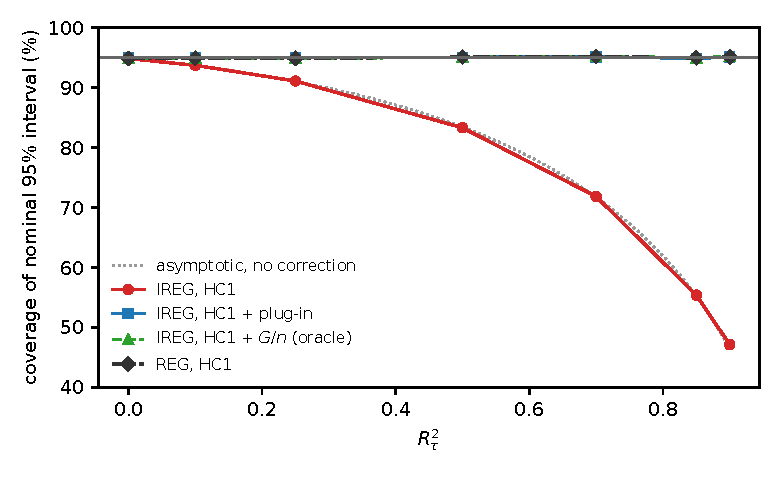
\includegraphics[width=0.75\textwidth]{figures/hte_coverage.pdf}
\caption{Coverage of nominal $95\%$ intervals against $R^2_\tau$ in the design of Table \ref{tab:hte}. The dotted curve is the asymptotic coverage of IREG without correction.}
\label{fig:hte}
\end{figure}

Table \ref{tab:hte} and Figure \ref{fig:hte} show the pattern. With $R^2_\tau=0$ every interval is close to nominal and the oracle does nothing. As $R^2_\tau$ grows, uncorrected IREG+HC1 undercovers more and more, from \gz{hte:sw:R2_0.10:IREG_HC1:cov}\% at $R^2_\tau=0.1$ to \gz{hte:sw:R2_0.50:IREG_HC1:cov}\% at $0.5$ and \gz{hte:sw:R2_0.90:IREG_HC1:cov}\% at $0.9$, tracking its asymptotic coverage. The oracle correction restores nominal coverage at every level (\gz{hte:sw:oracle:min}--\gz{hte:sw:oracle:max}\%), and the feasible correction stays within \gz{hte:sw:maxdev:c:o} points of the oracle, so in this design the plug-in estimates the population component it targets. REG+HC1, whose robust variance does not omit $G/n$, covers between \gz{hte:sw:reg:min}\% and \gz{hte:sw:reg:max}\% throughout. The corrected IREG interval widens as the component grows: at $R^2_\tau=0.9$ its median width is \gz{hte:sw:R2_0.90:IREG_HC1c:width} against \gz{hte:sw:R2_0.90:IREG_HC1:width} without the correction and \gz{hte:sw:R2_0.90:REG_HC1:width} for REG+HC1; the extra width is the genuine population uncertainty. HC3 does not address the omission: at $R^2_\tau=0.9$ IREG+HC3 covers \gz{hte:sw:R2_0.90:IREG_HC3:cov}\%, barely more than HC1. HC3 corrects leverage-driven finite-sample distortion of the variance estimate, whereas the $G/n$ correction accounts for sampling uncertainty that the fixed-design variance does not describe; they address different problems.

\subsection{Combined effects across designs}
\label{sec:combined}

The two mechanisms can coexist. Table \ref{tab:battery} applies the appropriate population-level implementation of IREG, HC1 plus the feasible correction, and the REG+HC1 benchmark to a battery of designs that combine Gaussian, misspecified, skewed and heavy-tailed covariates, heteroskedasticity, rare extreme values and different amounts of heterogeneity. All have $p=5$, $n=500$ and \gz{hte:reps} replications; they reuse the covariate and noise designs of the correction study (Appendix \ref{sec:supp-inference}), changing only the treatment-effect slope, and Table \ref{tab:battery-supp} adds uncorrected, oracle and HC3 intervals.

\begin{table}[htbp]
\centering
\caption{IREG with HC1 plus the feasible superpopulation correction against REG with HC1: coverage (\%) of nominal $95\%$ intervals for the population ATE and median interval width, with the MSE ratio of the point estimators ($p=5$, $n=500$; ``het.''\ denotes heteroskedastic noise). Designs are defined in Appendix \ref{sec:supp-inference}.}
\label{tab:battery}
\small
\setlength{\tabcolsep}{4pt}
\begin{tabular}{lrr|cc|cc}
\toprule
& & MSE ratio & \multicolumn{2}{c|}{IREG, HC1 + plug-in} & \multicolumn{2}{c}{REG, HC1} \\
Design & $R^2_\tau$ & IREG/REG & coverage & width & coverage & width \\
\midrule
\tablebody{tables/hte_battery_body.tex}
\bottomrule
\end{tabular}
\end{table}

In the Gaussian designs both procedures are close to nominal with small or large heterogeneity (corrected IREG \gz{hte:ba:gauss_low:IREG_HC1c:cov}\% and \gz{hte:ba:gauss_high:IREG_HC1c:cov}\%, REG+HC1 \gz{hte:ba:gauss_low:REG_HC1:cov}\% and \gz{hte:ba:gauss_high:REG_HC1:cov}\%). When $G=0$ there is no population component to recover, yet in the skewed design the correction raises IREG's coverage from \gz{hte:ba:skew_null:IREG_HC1:cov}\% to \gz{hte:ba:skew_null:IREG_HC1c:cov}\% through its finite-sample bias, offsetting part of the leverage effect of Section \ref{sec:gamma0}. As heterogeneity grows within the skewed family ($R^2_\tau=\gz{hte:ba:skew_low:R2}$, \gz{hte:ba:skew_mid:R2} and \gz{hte:ba:skew_high:R2}), uncorrected IREG+HC1 falls to \gz{hte:ba:skew_low:IREG_HC1:cov}\%, \gz{hte:ba:skew_mid:IREG_HC1:cov}\% and \gz{hte:ba:skew_high:IREG_HC1:cov}\%, and the feasible correction restores \gz{hte:ba:skew_low:IREG_HC1c:cov}\%, \gz{hte:ba:skew_mid:IREG_HC1c:cov}\% and \gz{hte:ba:skew_high:IREG_HC1c:cov}\%, close to the oracle; REG+HC1 stays near nominal at small and moderate heterogeneity but covers \gz{hte:ba:skew_high:REG_HC1:cov}\% at $R^2_\tau=\gz{hte:ba:skew_high:R2}$. The heavy-tailed designs show the mechanisms compounding: with large heterogeneity the corrected IREG interval covers \gz{hte:ba:heavy_high:IREG_HC1c:cov}\% and REG+HC1 only \gz{hte:ba:heavy_high:REG_HC1:cov}\%, because REG's residual now carries a heavy-tailed heterogeneity term; their HC3 versions cover \gz{hte:ba:heavy_high:IREG_HC3c:cov}\% and \gz{hte:ba:heavy_high:REG_HC3:cov}\% (Table \ref{tab:battery-supp}). In the rare-value design leverage and heterogeneity act together: uncorrected IREG+HC1 covers \gz{hte:ba:rare:IREG_HC1:cov}\%, the correction brings it to \gz{hte:ba:rare:IREG_HC1c:cov}\%, still below nominal, and REG+HC1 covers \gz{hte:ba:rare:REG_HC1:cov}\%. The MSE ratios, which concern the point estimators alone, vary in the same way: IREG is less precise in the skewed and heavy-tailed designs with little heterogeneity (ratios \gz{hte:ba:skew_null:mse}--\gz{hte:ba:heavy_low:mse}), the ratio is close to one in the Gaussian and skewed designs with large heterogeneity, IREG remains less precise in the heavy-tailed design even with large heterogeneity (\gz{hte:ba:heavy_high:mse}), and it is more precise in the rare-value design (\gz{hte:ba:rare:mse}).

\subsection{Practical implications}
\label{sec:practical}

The three experiments point to a few conclusions. When $G=0$, IREG's inference can still be fragile, because the arm-specific fit concentrates leverage on extreme covariate values and HC1 does not account for it; in the same designs IREG is also the less precise point estimator. HC3 substantially reduces this problem in most of the designs studied, but not in the heaviest tails, and it does nothing about the superpopulation omission. As heterogeneity grows, $G/n$ becomes a genuine first-order part of the uncertainty about the population ATE for centered IREG; the feasible correction then tracks the oracle, while with little or no heterogeneity it is dominated by its own finite-sample bias and can raise coverage for reasons unrelated to the estimand (Appendix \ref{sec:correction}). When heavy tails and heterogeneity occur together the two mechanisms compound, and REG's robust intervals are affected as well. Estimator choice and variance estimation therefore cannot be treated as separate decisions, and neither the simulations nor the theorem support a universal ranking of the two estimators.

\clearpage
\section{Discussion}

Regression adjustment in balanced trials involves three mechanisms that are easy to conflate, and the paper speaks to each separately.

\emph{Point-estimator efficiency.} REG and IREG have the same first-order variance when $\pi=1/2$, and Theorem \ref{theo:deficiency} gives the next term of the comparison. It depends on treatment-effect heterogeneity, covariate shape, residual heteroskedasticity and nonlinear misspecification, and it can favor either estimator. Under Gaussian covariates with homoskedastic, well-specified errors the second-order coefficient favors IREG and is linear in $p$ (for fixed $p$); with independent symmetric coordinates the ordering is decided by whether the kurtosis of the heterogeneity-driving covariate exceeds $p+4$; heteroskedasticity or misspecification add terms that can favor REG even without heterogeneity. The deficiency can be practically substantial: in the scalar lognormal family of Table \ref{tab:validity} it is \gz{def:s0.8} observations at $s=0.8$, \gz{def:s1.0} at $s=1$ and \gz{def:s1.2} at $s=1.2$, and at $n=500$ the simulated MSE of IREG exceeds that of REG by \gz{defsim:s1.0:n500}\% and \gz{defsim:s1.2:n500}\% in the last two designs. At $n=500$ the expansion overstates these gaps (it predicts \gz{defpred:s1.0:n500}\% and \gz{defpred:s1.2:n500}\%), but the agreement improves with $n$: at $n=8{,}000$ it predicts \gz{defpred:s1.0:n8000}\% against a simulated \gz{defsim:s1.0:n8000}\% for $s=1$. In the most heavy-tailed designs the finite-sample MSE gaps are larger still (the MSE ratio is $1.68$ (Monte Carlo SE \gz{mc:heavy:se}) in the heavy-tailed example of Section \ref{sec:intro} and \gz{samp:s2.0:mseratio} (SE \gz{samp:s2.0:mseratio:se}) in the $\gamma=0$, $s=2$ design of Section \ref{sec:gamma0}), but the $n^{-2}$ expansion no longer predicts their magnitude (Appendix \ref{sec:validity}). The sign of the comparison agrees with the expansion in every design where we compare the two (Tables \ref{tab:sampling}, \ref{tab:validation} and \ref{tab:validity} and the heavy-tailed example), so the decomposition of $D_p$ remains informative about direction beyond the range in which it is accurate about magnitude. Which estimator is preferable at second order thus depends on features of the data-generating process that first-order theory cannot see.

\emph{Estimand-level uncertainty.} For the population ATE, the first-order variance of the centered IREG estimator includes $G/n = R^2_\tau V^*/n$, which its conventional robust variance does not include; REG's robust variance has no such omission. This concerns what is being estimated, not the quality of a variance estimator. The feasible plug-in \eqref{eq:vsp} is biased upward by a term of leading order $\operatorname{tr}\{\Sigma_X\Var{\hdelta}\}/n$ that does not depend on $G$. When $G$ is small or zero this term can be large relative to the true component, so the plug-in can change coverage substantially for reasons unrelated to the estimand; a small $G$ does not make the feasible correction harmless.

\emph{Finite-sample variance estimation.} Even with $G=0$, the robust variance of IREG can be too small in finite samples. The pattern in our simulations is consistent with the leverage mechanism of \citet{ChesherJewitt1987}: the interacted specification creates high within-arm leverage for rare covariate values, and HC1 does not adjust for leverage. HC3 substantially improves coverage in most of our designs, but not under very heavy-tailed covariates, and at leverage-one observations no residual-based estimator can recover the observation's contribution. REG does not create the same arm-specific leverage problem, and its HC1 intervals are close to nominal at the $95\%$ level in the designs we examine, although in the most heavy-tailed designs they too are miscalibrated across nominal levels.

Section \ref{sec:practical} summarizes how these mechanisms co-vary with the size of treatment-effect heterogeneity in the designs we study.

None of these mechanisms explains the others. For practice, the upshot is that asymptotic efficiency of the point estimator does not determine the quality of the resulting confidence interval: the variance estimator actually used, the leverage structure of the fitted design, and the intended estimand each matter.

Several limitations remain. Our theorem holds $p$ fixed and does not cover settings in which the number of covariates grows with the sample size, the regime studied by \citet{lei2021regression} and \citet{ChiangMatsushitaOtsu2026} and the one in which parameter-count heuristics are most relevant. The second-order result is a statement about the expansion MSE of Definition \ref{def:msexp}; relating it to exact or trimmed moments requires conditions we do not verify. The inference results are numerical: we do not derive higher-order expansions for HC coverage in the sense of \citet{Rothenberg1988}, and the leverage-one results depend on the software's treatment of a $0/0$ contribution. We treat the superpopulation variance component of IREG only briefly (Section \ref{sec:estimand} and Appendix \ref{sec:correction}); the upward bias of the plug-in motivates a bias-corrected version, which we do not develop. The scale-versus-shape and width diagnostics of Appendix \ref{sec:supp-inference} are numerical. Finally, the main analysis is for balanced complete randomization; other treatment probabilities and designs remain open.

\section{Conclusion}

In balanced randomized experiments REG and IREG have the same first-order asymptotic variance, so their relative performance cannot be determined from standard efficiency theory alone. The main contribution of this paper is a closed-form second-order comparison: the difference in the $1/n^2$ terms of their expansion MSEs depends on treatment-effect heterogeneity, covariate shape, residual heteroskedasticity and nonlinear misspecification, can favor either estimator, and translates into an effective sample-size difference that ranges from a few observations to more than a hundred in our skewed scalar designs; in the most heavy-tailed designs the finite-sample gaps are larger still, but the expansion no longer predicts their magnitude.

As a practical companion, our simulations show that confidence intervals from standard software behave differently for the two estimators in finite samples. With no treatment-effect heterogeneity, interacted regression with HC1 standard errors can undercover substantially, in a pattern consistent with high within-arm leverage; HC3 substantially improves its coverage in most designs but not in the most extreme ones; and simple regression with HC1 is close to nominal at the $95\%$ level in the designs examined. Under superpopulation sampling, the variance of centered interacted regression for the population average treatment effect has an additional component, not included in its conventional robust variance, that matters when covariate-explained heterogeneity is large; in our large-heterogeneity design its plug-in estimate tracks the true component and restores calibration, with substantially wider intervals that reflect the added uncertainty, whereas with little or no heterogeneity the plug-in is noisy and miscalibrated across nominal levels.

These inference results are simulation evidence, not theorems. A higher-order theory of robust-variance coverage for regression adjustment, designs with a growing number of covariates, and unbalanced designs remain outside the scope of the paper.

\bibliographystyle{plainnat}
\bibliography{references}

\appendix

\section{Proofs}
\label{sec:proofs}

Throughout this appendix, Latin indices $i,j,k,l,a,b,c,d$ attached to $Z$, $T_3$, $T_4$, $\mathcal E$ and $P$ refer to \emph{coordinates} of the whitened covariate vector and are summed over in the Einstein convention; the unit index is suppressed. We write $G = \|\gamma\|^2$.

\subsection{Second-order expansion}

Under complete randomization with $n_1=m$ treated units, write $U_i^{(w)}$ for the vector collecting $X_i$, $Y_i(w)$ and the distinct entries of $X_iX_i^\top$ and $X_iY_i(w)$, and let $\bar U_1$ and $\bar U_0$ be the averages of $U_i^{(1)}$ over treated units and of $U_i^{(0)}$ over control units, with population means $\mu_1$ and $\mu_0$.

\begin{lemm}[Two-sample representation]
\label{lemm:two_sample}
Let $(X_i,Y_i(0),Y_i(1))$ be IID and let the assignment vector $W$ be independent of them, with $\sum_iW_i=m$. Conditionally on $W$, the treated observations $\{(X_i,Y_i(1)):W_i=1\}$ and the control observations $\{(X_i,Y_i(0)):W_i=0\}$ are independent IID samples of sizes $m$ and $n-m$ from the laws of $(X,Y(1))$ and $(X,Y(0))$. Both $\htau_\REG$ and $\htau_\IREG$ are of the form $h_{j,r}(\bar U_1,\bar U_0)$ with $r=m/n$, where $h_{j,r}$ is infinitely differentiable in a neighborhood of $(\mu_1,\mu_0)$ and its derivatives at $(\mu_1,\mu_0)$ are rational functions of $r$ without poles in $(0,1)$.
\end{lemm}

\begin{proof}
Given $W$, the units remain IID because $W$ is independent of them; the treated and control index sets are fixed and disjoint, so the two blocks are independent IID samples, observed through $Y_i(1)$ and $Y_i(0)$ respectively. Both estimators are rational functions of per-arm means, second moments and cross-moments: $\htau_\IREG$ is the difference of the arm-wise intercepts after centering at $\bar X=r\bar X_1+(1-r)\bar X_0$, with arm-wise least-squares slopes $\mathcal S_w^{-1}s_w$ built from $\bar U_w$; $\htau_\REG$ uses the pooled within-arm slope, whose Gram matrix is $r\mathcal S_1+(1-r)\mathcal S_0$. The Gram matrices are invertible at $(\mu_1,\mu_0)$ because $\Sigma\succ0$, which gives the smoothness and the dependence on $r$.
\end{proof}

\begin{lemm}[Conditional expansion]
\label{lemm:conditional}
Under Assumption \ref{assu:moments}, let $\MSEexp_{\CRT,r}(\htau_j)$ be the second moment of the third-order Taylor polynomial of $h_{j,r}$ at $(\mu_1,\mu_0)$. For every $\eta\in(0,\frac12)$,
\begin{equation}
\label{eq:conditional_expansion}
\MSEexp_{\CRT,r}(\hat{\tau}_{j}) = \frac{V_j(r)}{n}+\frac{c_j(r)}{n^2}+O(n^{-3}),
\qquad j\in\{\REG,\IREG\},
\end{equation}
uniformly in $r=m/n\in[\frac12-\eta,\frac12+\eta]$, with $V_j$ and $c_j$ infinitely differentiable in $r$.
\end{lemm}

\begin{proof}
The Taylor polynomial is a polynomial of degree three in $(\bar U_1-\mu_1,\bar U_0-\mu_0)$ whose coefficients are smooth in $r$ (Lemma \ref{lemm:two_sample}); its square has degree six. By Lemma \ref{lemm:two_sample} the two blocks are independent IID samples, so each mixed moment of the centered per-arm means is a finite sum of products of joint cumulants of $U^{(1)}$ and $U^{(0)}$ divided by powers of $m=rn$ and $n-m=(1-r)n$. Moments up to order six are finite because the entries of $U^{(w)}$ are products of at most two coordinates of $(X_i,Y_i(w))$ and Assumption \ref{assu:moments} bounds their twelfth moments. Collecting terms gives a finite expansion in powers of $1/n$ whose coefficients are rational in $r$ without poles on $[\frac12-\eta,\frac12+\eta]$; the terms beyond $n^{-2}$ are $O(n^{-3})$ uniformly on that interval.
\end{proof}

\begin{lemm}[Bernoulli and conditional expansions]
\label{lemm:bern_conditional}
Under Assumption \ref{assu:moments} with $W_i\stackrel{\mathrm{iid}}{\sim}\mathrm{Bernoulli}(1/2)$ independent of the units, let $\bar W=n^{-1}\sum_iW_i$. For every $\eta\in(0,\frac12)$,
\[
\MSEexp_\Bern(\htau_j) = \EEE\Big[\MSEexp_{\CRT,\bar W}(\htau_j)\,\mathbf 1\{|\bar W-\tfrac12|\le\eta\}\Big]+O(n^{-5/2}).
\]
\end{lemm}

\begin{proof}
Let $\mathcal P_\Bern$ be the Taylor polynomial of Definition \ref{def:msexp} under Bernoulli assignment and $\mathcal P_{\bar W}$ the conditional polynomial of Lemma \ref{lemm:conditional} evaluated at $r=\bar W$. Every coordinate of $\bar{\mathcal V}-\mu$ is a polynomial of degree at most two in $(\bar W-\frac12,\bar U_1-\mu_1,\bar U_0-\mu_0)$ and is linear in the per-arm means; for instance $n^{-1}\sum_iW_iU_i^{(1)}-\frac12\mu_1=(\bar W-\frac12)\mu_1+\frac12(\bar U_1-\mu_1)+(\bar W-\frac12)(\bar U_1-\mu_1)$. Hence $\EEE[(\mathcal P_\Bern-\tau)^2\mid W]$ is bounded uniformly in $W$, and since $\Pr(|\bar W-\frac12|>\eta)\le2e^{-2n\eta^2}$ by Hoeffding's inequality, the event $|\bar W-\frac12|>\eta$ contributes $O(e^{-2n\eta^2})$. On its complement, write $\htau_j=F_j(\bar W-\frac12,\bar U_1-\mu_1,\bar U_0-\mu_0)$ with $F_j$ smooth. Both $\mathcal P_\Bern$ and $\mathcal P_{\bar W}$ agree with the Taylor expansion of $F_j$ at the origin through total degree three, $\mathcal P_\Bern$ because the map to $\bar{\mathcal V}$ is polynomial and $\mathcal P_{\bar W}$ because it is exact in $\bar W$, so $\mathcal P_\Bern-\mathcal P_{\bar W}$ consists of terms of total degree at least four, each of which is at most cubic in the per-arm means. Conditionally on $\bar W$, the centered per-arm means are $O(n^{-1/2})$ in the $L^2$ norms that arise, and $\bar W-\frac12=O(n^{-1/2})$ in every $L^k$; hence $\|\mathcal P_\Bern-\mathcal P_{\bar W}\|_{L^2}=O(n^{-2})$ and $\|\mathcal P_\Bern+\mathcal P_{\bar W}-2\tau\|_{L^2}=O(n^{-1/2})$, and the Cauchy--Schwarz inequality gives $|\EEE[(\mathcal P_\Bern-\tau)^2-(\mathcal P_{\bar W}-\tau)^2]|=O(n^{-5/2})$ on that event.
\end{proof}

The proof of Theorem \ref{theo:deficiency} combines these lemmas, a reduction from the CRT to the Bernoulli design, and the Bernoulli calculation.

\begin{theo}
\label{theo:crt_reduction}
Suppose the Bernoulli design has second-order difference
\begin{equation}
\label{eq:bern_second_order}
\MSEexp_\Bern(\hat{\tau}_\IREG)-\MSEexp_\Bern(\hat{\tau}_\REG) = \frac{D_\Bern}{n^2}+O(n^{-5/2})
\end{equation}
at $\pi=1/2$, and let Assumption \ref{assu:moments} hold. Then, under complete randomization with $n_1=\lfloor n/2\rfloor$ treated units,
\begin{equation}
\label{eq:crt_second_order}
\MSEexp_\CRT(\hat{\tau}_\IREG)-\MSEexp_\CRT(\hat{\tau}_\REG) = \frac{D_\Bern+4G}{n^2}+O(n^{-5/2}).
\end{equation}
\end{theo}

\begin{proof}
Let $n_1=\sum_{i=1}^n W_i$ under the Bernoulli design and write $r=n_1/n$. Conditional on $n_1=m$, the treatment assignment has the same distribution as a CRT with treatment fraction $r$. Fix $\eta\in(0,\frac12)$. By Lemma \ref{lemm:bern_conditional}, $\MSEexp_\Bern$ is, up to $O(n^{-5/2})$, the average over $n_1$ of $\MSEexp_{\CRT,r}$ restricted to $|r-\frac12|\le\eta$, and by Lemma \ref{lemm:conditional} the latter admits the expansion \eqref{eq:conditional_expansion} uniformly on that set, with $V_j$ and $c_j$ infinitely differentiable. At treatment fraction $r$ the first-order variance difference is, by Proposition \ref{prop:first_order},
\[
V_{\IREG}(r)-V_{\REG}(r) = -\frac{(1-2r)^2}{r(1-r)}G,
\qquad
\frac{(1-2r)^2}{r(1-r)} = 16u^2+O(u^4),
\quad u = r-\tfrac12 .
\]
Under Bernoulli randomization with $\pi=1/2$, $\EEE[u^2]=1/(4n)$ and $\EEE[u^4]=O(n^{-2})$, so
\[
\frac{1}{n}\EEE\big[V_{\IREG}(r)-V_{\REG}(r)\big] = -\frac{4G}{n^2}+O(n^{-3}).
\]
For the second-order coefficients, a second-order Taylor expansion of $c_\IREG-c_\REG$ around $1/2$ together with $\EEE[u]=0$ and $\EEE[u^2]=O(n^{-1})$ gives $\EEE[c_{\IREG}(r)-c_{\REG}(r)] = c_{\IREG}(1/2)-c_{\REG}(1/2)+O(n^{-1})$. Averaging \eqref{eq:conditional_expansion} over $n_1$ therefore yields
\[
\MSEexp_{\Bern}(\hat{\tau}_{\IREG})-\MSEexp_{\Bern}(\hat{\tau}_{\REG}) = \frac{c_{\IREG}(1/2)-c_{\REG}(1/2)-4G}{n^2}+O(n^{-5/2}),
\]
so $D_{\Bern} = c_{\IREG}(1/2)-c_{\REG}(1/2)-4G$. Under balanced complete randomization $r=1/2$ for even $n$, giving $D_{\CRT} = c_{\IREG}(1/2)-c_{\REG}(1/2) = D_{\Bern}+4G$. For odd $n$, $r-1/2=O(n^{-1})$, so the induced change in the first-order variance difference is $O(n^{-3})$ and does not affect the $n^{-2}$ coefficient.
\end{proof}

\begin{theo}
\label{theo:bern_deficiency}
Let Assumption \ref{assu:moments} hold, except that $W_i\stackrel{\mathrm{iid}}{\sim}\text{Bernoulli}(1/2)$ independently of $(X_i,Y_i(0),Y_i(1))$. Define
\begin{align}
T_{3,ijk} &=\EEE[Z_iZ_jZ_k],
&
T_{4,ijkl} &=\EEE[Z_iZ_jZ_kZ_l],
&
q_i &=T_{3,ijk}\delta_{jk},
&
L_{ij} &=T_{3,iab}T_{3,jab},
\end{align}
write $S=q=\EEE[Z\|Z\|^2]$, and set $\mathcal E=\EEE[ZZ^\top\varepsilon]$ and $P=\EEE[ZZ^\top(W-\tfrac12)\varepsilon]$. For the scalar contractions
\begin{align}
G&=\|\gamma\|^2,
&
F&=\gamma_i\gamma_jT_{4,ijkk},
&
Q&=(\gamma^\top q)^2,
&
\mathcal R&=\gamma^\top L\gamma,
\\
A_P&=\gamma_iT_{3,ijk}P_{jk},
&
B_P&=(\gamma^\top q)\tr(P),
&
C_P&=\gamma^\top Pq,
\end{align}
we have
\begin{equation}
\label{eq:bern_mse_diff}
\MSEexp_{\Bern}(\hat{\tau}_\IREG)-\MSEexp_{\Bern}(\hat{\tau}_\REG) = \frac{D_{\Bern}}{n^2}+O(n^{-5/2}),
\end{equation}
where
\begin{equation}
\label{eq:Dbern}
D_{\Bern}
=
-(2p+7)G
+F-Q-3\mathcal R
-16A_P-8B_P+8C_P
+8\tr(\mathcal E^2)+8S^\top \EEE[Z\varepsilon^2].
\end{equation}
\end{theo}

\begin{proof}
Both REG and IREG contain the regressors $1$, $W$ and $X$. Subtracting any linear combination of these regressors from the outcome changes the fitted coefficient on $W$ by the corresponding amount while leaving the estimation error unchanged, so we may subtract the population main effects and the term $\tau W_i$ and work with the exact representation $Y_i=W_i X_i^\top\{\beta^*_{(1)}-\beta^*_{(0)}\}+\varepsilon_i$. Whitening as in \eqref{eq:whitening} gives the canonical representation $Y_i=W_i\gamma^\top Z_i+\varepsilon_i$, and we write
\[
W_i=\tfrac12+\omega_i,
\qquad
\omega_i\in\{-\tfrac12,\tfrac12\},
\qquad
\EEE[\omega_i]=0,
\qquad
\omega_i^2=\tfrac14 .
\]

Let $\mathcal V_i$ denote the vector of raw-moment coordinates needed to evaluate the REG or IREG coefficient map, and adopt the notation of Definition \ref{def:msexp}, so that $\htau = g(\bar{\mathcal V})$ and $\tilde\tau_n$ is given by \eqref{eq:hall_expansion}. Let
\[
\Sigma^{\mathcal V}_{ij}=\Cov(\mathcal V_i,\mathcal V_j),
\qquad
\mu^{\mathcal V}_{3,ijk}=\EEE[(\mathcal V_i-\mu_i)(\mathcal V_j-\mu_j)(\mathcal V_k-\mu_k)]
\]
be the covariance and third central-moment tensors of the moment vector. Expanding the square of \eqref{eq:hall_expansion} and using the second- and third-order moments of sample means gives the order-$n^{-1}$ correction to $n\MSEexp$ as $\mathcal T_1+\mathcal T_2+\mathcal T_3$ with
\begin{equation}
\label{eq:hall_T1}
\mathcal T_1=a_iH_{jk}\mu^{\mathcal V}_{3,ijk},
\end{equation}
\begin{equation}
\label{eq:hall_T2_bern}
\mathcal T_2 = \frac14 H_{ij}H_{kl}\p{\Sigma^{\mathcal V}_{ik}\Sigma^{\mathcal V}_{jl}+\Sigma^{\mathcal V}_{il}\Sigma^{\mathcal V}_{jk}+\Sigma^{\mathcal V}_{ij}\Sigma^{\mathcal V}_{kl}},
\end{equation}
\begin{equation}
\label{eq:hall_T3_bern}
\mathcal T_3 = \frac13 a_iA_{3,jkl}\p{\Sigma^{\mathcal V}_{ij}\Sigma^{\mathcal V}_{kl}+\Sigma^{\mathcal V}_{ik}\Sigma^{\mathcal V}_{jl}+\Sigma^{\mathcal V}_{il}\Sigma^{\mathcal V}_{jk}},
\end{equation}
the remaining terms being $O(n^{-3/2})$ in $n\MSEexp$ under Assumption \ref{assu:moments}. The difference between the order-$n^{-2}$ MSE coefficients of REG and IREG is obtained by evaluating these three contractions for the two estimators.

The population Gram matrices and their inverses in the whitened coordinates are
\[
A_R=
\begin{pmatrix}
1&0&1/2\\
0&I_p&0\\
1/2&0&1/2
\end{pmatrix},
\quad
A_R^{-1}=
\begin{pmatrix}
2&0&-2\\
0&I_p&0\\
-2&0&4
\end{pmatrix},
\quad
A_I=
\begin{pmatrix}
1&0&1/2&0\\
0&I_p&0&I_p/2\\
1/2&0&1/2&0\\
0&I_p/2&0&I_p/2
\end{pmatrix},
\]
\[
A_I^{-1}=
\begin{pmatrix}
2&0&-2&0\\
0&2I_p&0&-2I_p\\
-2&0&4&0\\
0&-2I_p&0&4I_p
\end{pmatrix},
\qquad
\theta_R=(0,\gamma/2,0),
\qquad
\theta_I=(0,0,0,\gamma).
\]
Writing $\Omega=A^{-1}$ and $\theta=\Omega b$, differentiation of $A\theta=b$ gives the exact derivative identities
\[
D\theta[h] = \Omega(db-dA\,\theta),
\qquad
D^2\theta[h_1,h_2] = -\Omega dA_1\Omega(db_2-dA_2\theta)-\Omega dA_2\Omega(db_1-dA_1\theta),
\]
\[
D^3\theta[h_1,h_2,h_3] = \sum_{\varsigma\in\mathfrak S_3} \Omega dA_{\varsigma_1}\Omega dA_{\varsigma_2}\Omega(db_{\varsigma_3}-dA_{\varsigma_3}\theta).
\]
REG's estimator is the treatment coefficient, $g_\REG(v)=\theta_W(v)$. IREG's is $g_\IREG(v)=\theta_W(v)+\bar z(v)^\top\theta_{WZ}(v)$, where $\bar z(v)$ is the full-sample covariate mean, a linear coordinate of $v$ that vanishes at $\mu$ in whitened coordinates, and $\theta_{WZ}=\gamma$ at $\mu$. The product rule gives
\[
a_\IREG[h]=D\theta_W[h]+D\bar z[h]^\top\gamma,
\]
\[
H_\IREG[h_1,h_2]=D^2\theta_W[h_1,h_2]+D\bar z[h_1]^\top D\theta_{WZ}[h_2]+D\bar z[h_2]^\top D\theta_{WZ}[h_1],
\]
\[
A_{3,\IREG}[h_1,h_2,h_3]=D^3\theta_W[h_1,h_2,h_3]+\textstyle\sum_{\{i,j,k\}=\{1,2,3\}} D\bar z[h_i]^\top D^2\theta_{WZ}[h_j,h_k],
\]
the sum running over the three choices of $i$. The covariance and third-moment blocks of $\mathcal V_i$ are products of moments of $(Z_i,\omega_i,\varepsilon_i)$ under the canonical representation of Section \ref{sec:asymptotics}, with $W_i$ marginally Bernoulli$(1/2)$.

Substituting these derivative tensors and the covariance and third-moment blocks of $\mathcal V_i$ into \eqref{eq:hall_T1}--\eqref{eq:hall_T3_bern}, and reducing the resulting indexed sums using $\EEE[\omega_i]=0$, $\omega_i^2=1/4$, the four population normal equations for $\varepsilon_i$ and the symmetries of $T_3$ and $T_4$, gives
\begin{align}
\Delta\mathcal T_1 &= 2G+2F+8\Xi_\gamma, \label{eq:dT1}\\
\Delta\mathcal T_2 &= -3G-F-Q-\mathcal R-8\Xi_\gamma-8A_P-8B_P, \label{eq:dT2}\\
\Delta\mathcal T_3 &= -(2p+6)G-2\mathcal R-8A_P+8C_P+8\tr(\mathcal E^2)+8S^\top \EEE[Z\varepsilon^2], \label{eq:dT3}
\end{align}
where $\Xi_\gamma = \EEE[(\gamma^\top Z)\|Z\|^2\omega\varepsilon]$ with $\omega=W-\frac12$. The algebra in \eqref{eq:dT1}--\eqref{eq:dT3} is carried out symbolically: the reference implementation enumerates the full Cartesian products of the expansion directions, applies the derivative tensors above, and reduces the resulting indexed expressions using only tensor symmetries, dummy-index relabeling and the identities implied by $\EEE[ZZ^\top]=I_p$ and $\omega_i^2=1/4$, with the dimension $p$ kept symbolic. The symbolic remainder for each of the three rows is identically zero; the certificate is \texttt{verification/general\char`\_p\char`\_symbolic\char`\_certificate.py} in the replication repository and runs in under a minute.

Summing the three rows, the $\Xi_\gamma$ terms cancel and \eqref{eq:Dbern} follows.

The division of labour is as follows. Derived by hand and displayed above: the expansion terms \eqref{eq:hall_T1}--\eqref{eq:hall_T3_bern}, the Gram matrices and coefficients at $\mu$, the derivative identities, the product-rule structure of the IREG centering functional, and the reduction rules. Machine-checked: the substitution of these objects into \eqref{eq:hall_T1}--\eqref{eq:hall_T3_bern} and the reduction of the resulting indexed sums to the rows \eqref{eq:dT1}--\eqref{eq:dT3}, which \texttt{verification/general\char`\_p\char`\_symbolic\char`\_certificate.py} carries out for symbolic $p$ with a zero remainder. The resulting constant is checked independently by Monte Carlo in Appendix \ref{sec:numerical-verification}.
\end{proof}

Theorems \ref{theo:crt_reduction} and \ref{theo:bern_deficiency} give
\begin{equation}
\label{eq:unsimp}
D_p = -(2p+3)G+F-Q-3\mathcal R-16A_P-8B_P+8C_P+8\tr(\mathcal E^2)+8S^\top \EEE[Z\varepsilon^2],
\end{equation}
which Lemma \ref{lemm:matrix} rewrites in the matrix form of Theorem \ref{theo:deficiency}.

\begin{lemm}[Equivalent matrix form]
\label{lemm:matrix}
With $K$, $S$, $S_\gamma$, $\mathcal E$ and $\mathcal E_W$ as in Theorem \ref{theo:deficiency},
\[
G=\|\gamma\|^2,
\quad
F=\gamma^\top K\gamma,
\quad
Q=(\gamma^\top S)^2,
\quad
\mathcal R=\|S_\gamma\|_F^2,
\]
\[
A_P=\tr(S_\gamma \mathcal E_W),
\quad
B_P=(\gamma^\top S)\tr(\mathcal E_W),
\quad
C_P=\gamma^\top \mathcal E_WS.
\]
\end{lemm}

\begin{proof}
First, $F=\gamma_i\gamma_jT_{4,ijkl}\delta_{kl}=\gamma^\top\EEE[ZZ^\top\|Z\|^2]\gamma=\gamma^\top K\gamma$, and $S=\EEE[Z_iZ_jZ_j]_{i=1}^p=q$ gives $Q=(\gamma^\top q)^2=(\gamma^\top S)^2$. Next, $(S_\gamma)_{ab}=\EEE[Z_aZ_b(Z^\top\gamma)]=T_{3,abk}\gamma_k$, so
\[
\|S_\gamma\|_F^2=\sum_{a,b}(S_\gamma)_{ab}^2=\gamma_k\gamma_\ell T_{3,abk}T_{3,ab\ell}=\gamma_k\gamma_\ell L_{k\ell}=\mathcal R.
\]
Since $S_\gamma$ and $\mathcal E_W$ are symmetric, $\tr(S_\gamma \mathcal E_W)=(S_\gamma)_{jk}(\mathcal E_W)_{jk}=\gamma_iT_{3,ijk}P_{jk}=A_P$; finally $B_P=(\gamma^\top q)\tr(P)=(\gamma^\top S)\tr(\mathcal E_W)$ and $C_P=\gamma^\top Pq=\gamma^\top \mathcal E_WS$.
\end{proof}

We close with an exact identity that is used by the variance-reduced verification of Appendix \ref{sec:numerical-verification}.

\begin{lemm}[Exact difference identity]
\label{lemm:exact_diff}
Let $\bar X_w$ and $\mathcal S_w=\sum_{i:W_i=w}(X_i-\bar X_w)(X_i-\bar X_w)^\top$ denote the within-arm means and scatter matrices, let $\hbeta_w=\mathcal S_w^{-1}\sum_{i:W_i=w}(X_i-\bar X_w)(Y_i-\bar Y_w)$, and write $d_X=\bar X_1-\bar X_0$. Then, whenever $\mathcal S_0$, $\mathcal S_1$ and $\mathcal S_0+\mathcal S_1$ are invertible and $n_1=n_0$,
\[
\htau_\REG = \bar Y_1-\bar Y_0-d_X^\top (\mathcal S_1+\mathcal S_0)^{-1}(\mathcal S_1\hbeta_1+\mathcal S_0\hbeta_0),
\qquad
\htau_\IREG = \bar Y_1-\bar Y_0-d_X^\top \frac{\hbeta_1+\hbeta_0}{2},
\]
and consequently
\[
\htau_\IREG-\htau_\REG = \tfrac12\,d_X^\top (\mathcal S_1+\mathcal S_0)^{-1}(\mathcal S_1-\mathcal S_0)(\hbeta_1-\hbeta_0) = O_P(n^{-1}).
\]
\end{lemm}

\begin{proof}
Both expressions for the estimators are the Frisch--Waugh--Lovell representations of \eqref{eq:estimators}: the coefficient on $X$ in the REG regression is the pooled within-arm slope $(\mathcal S_1+\mathcal S_0)^{-1}(\mathcal S_1\hbeta_1+\mathcal S_0\hbeta_0)$, and IREG fits the two arms separately, so with $n_1 = n_0$ the overall covariate mean satisfies $\bar X_1 - \bar X = d_X/2 = -(\bar X_0 - \bar X)$. Subtracting,
\[
\htau_\IREG-\htau_\REG = d_X^\top\Big[(\mathcal S_1+\mathcal S_0)^{-1}(\mathcal S_1\hbeta_1+\mathcal S_0\hbeta_0) - \tfrac12(\hbeta_1+\hbeta_0)\Big]
= \tfrac12d_X^\top(\mathcal S_1+\mathcal S_0)^{-1}(\mathcal S_1-\mathcal S_0)(\hbeta_1-\hbeta_0).
\]
The stochastic order follows from $d_X = O_P(n^{-1/2})$, $(\mathcal S_1+\mathcal S_0)^{-1}(\mathcal S_1-\mathcal S_0) = O_P(n^{-1/2})$ and $\hbeta_1-\hbeta_0 = O_P(1)$.
\end{proof}

In whitened coordinates the leading term of this difference is $\tfrac14d_Z^\top(A_1-A_0)\gamma$, with $A_w$ the arm-$w$ mean of $ZZ^\top-I_p$; this is the control variate used in \eqref{eq:cv_identity} below.


\begin{lemm}[Leading expansion bias]
\label{lemm:bias}
Under Assumption \ref{assu:moments} and balanced complete randomization,
\[
\EEE[\tilde\tau_{n,\IREG}-\tau]=-\frac{4\tr(\mathcal E_W)}{n}+O(n^{-2}),
\qquad
\EEE[\tilde\tau_{n,\REG}-\tau]=-\frac{4\tr(\mathcal E_W)+\gamma^\top S}{n}+O(n^{-2}).
\]
\end{lemm}

\begin{proof}
Work in whitened coordinates with $m=n/2$ units per arm, arm slopes $b_1-b_0=\gamma$, projection residuals $\varepsilon_i(w)$ and within-arm scatter matrices $\mathcal S_w$. By Remark \ref{rema:bias}, the expansion bias is the mean of the quadratic part of $\htau-\tau$, up to $O(n^{-2})$. For IREG, $\bar Z_1-\bar Z=-(\bar Z_0-\bar Z)=\frac12(\bar Z_1-\bar Z_0)$, so
\[
\htau_\IREG-\tau=\bar\varepsilon_1-\bar\varepsilon_0+\gamma^\top\bar Z-\tfrac12(\bar Z_1-\bar Z_0)^\top\{(\hat b_1-b_1)+(\hat b_0-b_0)\},
\]
and the linear part of $\hat b_w-b_w$ is $m^{-1}\sum_{i:W_i=w}Z_i\varepsilon_i(w)$, which enters the quadratic part of $\htau_\IREG-\tau$ through its product with $\bar Z_1-\bar Z_0$. The arms are independent (Lemma \ref{lemm:two_sample}), so $\EEE[(\bar Z_1-\bar Z_0)^\top(\hat b_1-b_1)]=m^{-1}\EEE[\|Z\|^2\varepsilon(1)]+O(n^{-2})$ and $\EEE[(\bar Z_1-\bar Z_0)^\top(\hat b_0-b_0)]=-m^{-1}\EEE[\|Z\|^2\varepsilon(0)]+O(n^{-2})$, which gives $-(2m)^{-1}\tr\{\EEE[ZZ^\top\varepsilon(1)]-\EEE[ZZ^\top\varepsilon(0)]\}=-4\tr(\mathcal E_W)/n$. For REG, the pooled slope $\hat b$ estimates $\bar b=(b_1+b_0)/2$ and
\[
\htau_\REG-\tau=\bar\varepsilon_1-\bar\varepsilon_0+\tfrac12\gamma^\top(\bar Z_1+\bar Z_0)-(\bar Z_1-\bar Z_0)^\top(\hat b-\bar b).
\]
The pooled residual of unit $i$ is $\varepsilon_i(W_i)+(W_i-\frac12)\gamma^\top Z_i$ up to centering, so the linear part of $\hat b-\bar b$ is $n^{-1}\sum_iZ_i\{\varepsilon_i(W_i)+(W_i-\frac12)\gamma^\top Z_i\}$, which again enters the quadratic part of $\htau_\REG-\tau$ through its product with $\bar Z_1-\bar Z_0$, and $\EEE[(\bar Z_1-\bar Z_0)^\top(\hat b-\bar b)]=n^{-1}\{\tr\EEE[ZZ^\top\varepsilon(1)]-\tr\EEE[ZZ^\top\varepsilon(0)]+\gamma^\top S\}+O(n^{-2})$, which gives the second display.
\end{proof}

\section{Numerical verification of Theorem \ref{theo:deficiency}}
\label{sec:numerical-verification}

The symbolic certificate establishes the algebra of Theorem \ref{theo:bern_deficiency} exactly. The role of simulation is therefore not to re-derive $D_p$ but to provide an independent numerical check that the constant governs the sampling behavior of the estimators: that we expanded the right quantity, that the CRT correction of Theorem \ref{theo:crt_reduction} is right, and that no term was lost in translation. Simulation cannot prove the theorem; we design the checks so that they can fail, and report their power.

\paragraph{Exact targets.}
The verification uses data-generating processes whose whitened covariates have independent coordinates with known moments and whose oracle residuals take the form $\varepsilon(w)=g_w(Z)+s_w(Z)\eta$, with $\eta$ independent of $Z$ with mean zero and unit variance, $g_w$ a polynomial orthogonal to $(1,Z)$ and $s_w^2$ a polynomial. Every ingredient of $D_p$ is then a finite sum of moments, computed in exact rational arithmetic, so the target carries no Monte Carlo error; the code also verifies $\EEE[g_w]=\EEE[Zg_w]=0$ so that a mis-specified design cannot pass silently. These distributions are chosen for analytic tractability and are deliberately different from the designs of Section \ref{sec:gamma0}. Six are used, so that every block of $D_p$ is active in at least one: Gaussian homoskedastic ($F$ only); centered-exponential covariates with heterogeneity ($F,Q,\mathcal R$); centered-exponential covariates with heteroskedasticity and $\gamma=0$ (the $8S^\top\EEE[Z\varepsilon^2]$ block alone); centered-exponential covariates with heterogeneity, arm-specific misspecification and arm-specific heteroskedasticity (all nine terms, including $A_P$, $B_P$ and $C_P$); Gaussian covariates with arm-specific misspecification and heteroskedasticity ($\tr(\mathcal E^2)$ and $\mathcal E_W$); and a mixed skewed/Gaussian design.

\paragraph{A variance-reduced estimator of $D_p$.}
The natural estimator $n^2\{\widehat\MSE_\IREG-\widehat\MSE_\REG\}$ is badly behaved: by Lemma \ref{lemm:exact_diff} the difference of the estimators is $O_P(n^{-1})$ while $\htau_\REG-\tau=O_P(n^{-1/2})$, so the per-replication standard deviation of the statistic grows like $\sqrt n$ and confidence intervals become \emph{wider} as $n$ grows at fixed replication count. We therefore subtract an exactly-centered control variate. With $d_Z=\bar Z_1-\bar Z_0$, $A_w$ the arm-$w$ mean of $ZZ^\top - I_p$, and
\[
d_1=\tfrac14d_Z^\top(A_1-A_0)\gamma,
\qquad
L=\gamma^\top\bar Z+\bar\varepsilon_1-\bar\varepsilon_0,
\]
the expectation of a product of three centered IID sample means over an arm of size $m=n/2$ equals the corresponding third cumulant divided by $m^2$, which gives the exact finite-$n$ identity
\begin{equation}
\label{eq:cv_identity}
\EEE[d_1 L]
=
\frac{1}{n^2}\,
\EEE\Big[\big(\|Z\|^2-1\big)\,(\gamma^\top Z)\,\big(\gamma^\top Z+\varepsilon(1)-\varepsilon(0)\big)\Big].
\end{equation}
The estimator
\[
\hat D_p
=
\frac1B\sum_{b=1}^B\Big[n^2\big(e_{\IREG,b}^2-e_{\REG,b}^2\big)-2n^2d_{1,b}L_b\Big]
+
2n^2\,\EEE[d_1L]
\]
is unbiased for the same quantity as the raw statistic, with per-replication variance $O(1)$ rather than $O(n)$. Both are reported by the replication code: in the Gaussian design the raw per-replication standard deviation grows from $151$ at $n=200$ to $293$ at $n=800$, while the control-variate standard deviation is $56$ and $55$; at $n=3200$ the control-variate standard error is ten times smaller than the raw one.

\paragraph{Results.}
Table \ref{tab:validation} reports the exact targets and the control-variate estimates at $n\in\{200,800,3200\}$, with $B=400{,}000$ replications at the two smaller sample sizes and $B=120{,}000$ at the largest. Because the control-variate estimator has per-replication standard deviation of order one, it resolves the finite-$n$ remainder: at $n=200$ several designs lie many standard errors from their targets, up to $22$ in the design with all blocks active. These deviations shrink as $n$ grows; in that design the gap to the target falls from $12.1$ to $5.7$ to $2.6$ as $n$ quadruples twice. In that design $D_\Bern=D_p-4G=\gz{val:full:dbern}$ lies within one standard error of the estimate at $n=3{,}200$, so this design alone does not separate $D_p$ from $D_\Bern$ at that sample size. Its successive increments, \gz{val:full:inc1} and \gz{val:full:inc2}, roughly halve as $n$ quadruples, which extrapolates to about \gz{val:full:extrap}, close to $D_p$; the ablation in Table \ref{tab:ablation} separates the two decisively in other designs. At $n=3200$ every estimate is within $2.6$ standard errors of its target. The two largest deviations are $-2.6$ in the all-blocks design, whose trajectory is still approaching the target from below, and $+2.3$ in the $\gamma=0$ heteroskedastic design, which lies below its target at $n=200$ and $n=800$ and above it at $n=3200$; with six designs, a deviation of this size is unremarkable under Monte Carlo error. The deviations are consistent with a remainder that vanishes relative to $n^{-2}$ in the untrimmed MSE difference, but with three sample sizes we do not attempt to estimate its rate.

\begin{table}[htbp]
\centering
\caption{Verification of Theorem \ref{theo:deficiency}. Targets are exact; estimates are the control-variate estimator with Monte Carlo standard errors in parentheses. $B=400{,}000$ for $n\in\{200,800\}$ and $B=120{,}000$ for $n=3200$.}
\label{tab:validation}
\small
\resizebox{\textwidth}{!}{%
\begin{tabular}{lrrrr}
\toprule
DGP (active blocks) & $D_p$ (exact) & $n=200$ & $n=800$ & $n=3200$ \\
\midrule
\tablebody{tables/validation_body.tex}
\bottomrule
\end{tabular}}
\end{table}

\paragraph{Power: what the verification would reject.}
A check that cannot fail is not evidence. Table \ref{tab:ablation} reports $z$-statistics of the $n=3200$ estimates against deliberately perturbed versions of the formula: the Bernoulli constant $D_\Bern=D_p-4G$ (that is, omitting Theorem \ref{theo:crt_reduction}), the Gaussian special case $-(p+1)G$, and $D_p$ with individual blocks deleted. The constant of Theorem \ref{theo:deficiency} has $|z|\leq 2.6$ in every design, while each alternative has $|z|>3$ in at least one design, in several cases by tens of standard errors. The check has limited power against alternatives that differ from $D_p$ by less than the residual finite-$n$ bias: in the all-blocks design, for example, $D_\Bern = D_p - 3.2$ is not separated from $D_p$ at $n=3200$, which is why several designs are needed. A conventional Monte Carlo design without the control variate would have standard errors of $2$--$12$ on these quantities and could not separate most of the alternatives.

\begin{table}[htbp]
\centering
\caption{Ablation: $z=(\hat D_p - D^{\mathrm{alt}})/\widehat{SE}$ at $n=3200$ for each design and each candidate constant. Values with $|z|>3$ indicate rejection of that candidate.}
\label{tab:ablation}
\small
\setlength{\tabcolsep}{4pt}
\resizebox{\textwidth}{!}{%
\begin{tabular}{lrrrrrrr}
\toprule
DGP & $D_p$ & $D_p-4G$ & $-(p+1)G$ & drop $-3\mathcal R$ & drop $-Q$ & drop resid.\ & drop $\mathcal E_W$ \\
\midrule
\tablebody{tables/ablation_body.tex}
\bottomrule
\end{tabular}}
\end{table}

\paragraph{The CRT correction and the bias decomposition.}
Theorem \ref{theo:crt_reduction} is checked separately by estimating the $n^{-2}$ constant under both the balanced CRT and Bernoulli$(1/2)$ assignment on the same designs (\texttt{verification/crt\char`\_correction\char`\_certificate.py}): the estimated gap between the two designs is $4.3\pm0.6$ at $n=200$ and $6.3\pm1.6$ at $n=800$ in the Gaussian design, and $3.0\pm1.1$ and $8.6\pm3.0$ in the exponential-covariate design, against the predicted $4G=5$ in both, with all four $|z|<2$. This check uses the raw statistic, because the control variate is derived for the two-independent-samples representation of the CRT, so its power is modest; the ablation in Table \ref{tab:ablation}, which rejects $D_\Bern$ by up to thirty standard errors, is the sharper test. Remark \ref{rema:bias} is checked by estimating the biases of both estimators directly (\texttt{simulations/run\char`\_bias.py}): with $10^6$ replications, at $n=800$ all six estimated biases (REG and IREG in three designs) are within $0.8$ Monte Carlo standard errors of the leading-order predictions; at $n=200$ the all-blocks design deviates by about $11\%$ of the predicted REG bias ($z=9.3$), a gap that has disappeared at $n=800$ ($z=0.4$), consistent with the $O(n^{-2})$ remainder of Lemma \ref{lemm:bias}.

\section{Range of validity of the second-order approximation}
\label{sec:validity}

Theorem \ref{theo:deficiency} describes the limit $n\to\infty$; separately from whether $D_p$ is correct, one should ask when $1+\Delta/n$ is a usable approximation to the finite-sample MSE ratio. Because $\Delta$ is driven by third and fourth moments of the whitened covariates, and those same moments control the size of the neglected terms, the two questions are linked. Table \ref{tab:validity} makes the trade-off explicit in the scalar lognormal family of the introduction, with $\sigma(X)=1+X$ and treatment-effect slope $0.4$ held fixed and only the log-scale $s$ of $X\sim\mathrm{LogNormal}(0,s^2)$ varying.

\begin{table}[htbp]
\centering
\caption{Simulated MSE ratio $\widehat\MSE_\IREG/\widehat\MSE_\REG$ versus the second-order prediction $1+\Delta/n$, for $X\sim\mathrm{LogNormal}(0,s^2)$, $\sigma(X)=1+X$, treatment-effect slope $0.4$. Monte Carlo standard errors of the simulated ratios are given in parentheses in units of the last reported digit. This family has $\sigma(X)=1+X$; the introductory example ($\sigma(X)=1+2X$) and its heavy-tailed variant ($\sigma(X)=1+1.5X$, slope $0.3$) are separate designs.}
\label{tab:validity}
\small
\begin{tabular}{rrrrrrrrr}
\toprule
 & & & \multicolumn{2}{c}{$n=500$} & \multicolumn{2}{c}{$n=2000$} & \multicolumn{2}{c}{$n=8000$} \\
$s$ & skew $Z$ & $\Delta$ & sim. & pred. & sim. & pred. & sim. & pred. \\
\midrule
\tablebody{tables/validity_body.tex}
\bottomrule
\end{tabular}
\end{table}

Within this family, for $s=0.8$ (skewness $3.7$) the simulated excess MSE is \gz{valid:s0.8:n500:frac}\% of the predicted excess $\Delta/n$ at $n=500$ and \gz{valid:s0.8:n2000:frac}\% at $n=2{,}000$ (for $s=0.6$, \gz{valid:s0.6:n500:frac}\% and \gz{valid:s0.6:n2000:frac}\%); the prediction progressively overstates the gap as the tail becomes heavier; at $s=1.5$ the predicted ratio exceeds the simulated one by a factor of four at $n=500$. We do not claim that this boundary transfers to other families of distributions. In the heavy-tailed variant of the introductory example ($s=1.8$, $\sigma(X)=1+1.5X$, slope $0.3$), $\Delta\approx 3.9\times 10^4$ and $1+\Delta/n$ exceeds the simulated ratio by a factor of more than forty at $n=500$: the ordering is right and REG's advantage is real (the simulated MSE ratio is $1.68$ at $n=500$, $1.34$ at $n=2{,}000$ and $1.19$ at $n=8{,}000$, against predictions of $78.5$, $20.4$ and $5.8$), but the deficiency is no longer a useful numerical summary. That regime is also where HC1 intervals fail for IREG: in this design ($R^2_\tau\approx0.009$), IREG+HC1 covers $\tau$ in $85.6\%$ of replications, IREG+HC2 in $88.9\%$ and IREG+HC3 in $94.0\%$, against $94.4\%$ for REG+HC1 and $96.7\%$ for REG+HC3.

\paragraph{Tail sensitivity.} In the heaviest designs the deficiency is dominated by covariate values far in the tail. Table \ref{tab:tail} recomputes $1+\Delta/n$ at $n=500$ after truncating the lognormal law at a high quantile, for which the moments entering $\Delta$ have closed forms. Truncation at the $1-10^{-4}$ quantile reduces $\Delta$ by one to three orders of magnitude, so $\Delta$ is dominated by far-tail moments. The simulations draw between $10^7$ and $5\times10^7$ covariate values and so reach roughly the $1-10^{-7}$ quantile, yet even the law truncated at the $1-10^{-8}$ quantile gives predictions several times the simulated ratio. In these rows the expansion is inaccurate already at leading order: in the $\gamma=0$ designs the simulated standard deviation of $\htau_\REG$ matches $\sqrt{V^*/n}$ at $s=0.6$ (\gz{samp:s0.6:sdR} against \gz{samp:s0.6:sdtheory}) but is \gz{samp:s1.5:sdR} against \gz{samp:s1.5:sdtheory} at $s=1.5$ and \gz{samp:s2.0:sdR} against \gz{samp:s2.0:sdtheory} at $s=2$ (Table \ref{tab:sampling}), so their finite-sample behavior lies outside the perturbative regime of the expansion. The discrepancy is therefore primarily a failure of the $n^{-2}$ approximation to predict the magnitude of the gap in these designs; Monte Carlo error in the heaviest rows, whose simulated MSEs are dominated by rare draws, is a secondary source of uncertainty. The sign of the comparison agrees in every design.

\begin{table}[htbp]
\centering
\caption{Second-order prediction $1+\Delta/n$ at $n=500$ for the full lognormal law and for its truncation at the $q$ quantile, against the simulated MSE ratio (Monte Carlo standard error in parentheses, in units of the last digit).}
\label{tab:tail}
\small
\setlength{\tabcolsep}{4pt}
\begin{tabular}{lccccc}
\toprule
& Simulated & \multicolumn{4}{c}{$1+\Delta/n$} \\
Design & ratio & full law & $q=1-10^{-4}$ & $q=1-10^{-6}$ & $q=1-10^{-8}$ \\
\midrule
\tablebody{tables/tail_body.tex}
\bottomrule
\end{tabular}
\end{table}

\section{Implementation and validation of the inference simulations}
\label{sec:r-validation}

The simulations of Section \ref{sec:feasible} are implemented in R (\texttt{r/gamma0\char`\_sim.R}). For each replication, the design matrices are built exactly as \texttt{lm\char`\_robust(y \textasciitilde{} w + x)} and \texttt{lm\char`\_lin(y \textasciitilde{} w, covariates = \textasciitilde{} x)} build them, and the fits are computed by \texttt{estimatr}'s own fitting routine, the function those two interfaces call; intervals use the degrees of freedom \texttt{estimatr} reports. Without clustering, \texttt{estimatr}'s default is HC2, motivated by its connection to Neyman's variance estimator \citep{samii2012equivalencies}; we request HC1 and HC3 explicitly. The main runs use \texttt{estimatr} \gz{estimatr:v1}; the rare-value design is repeated with \texttt{estimatr} \gz{estimatr:v2}. The validation script \texttt{r/validate\char`\_estimatr.R} and the Python cross-check \texttt{simulations/crosscheck\char`\_r.py} establish the following, under both versions.
\begin{itemize}
\item On \gz{val:datasets} simulated datasets from four designs, the formula interfaces \texttt{lm\char`\_robust} and \texttt{lm\char`\_lin} and the simulation engine give identical estimates, HC1--HC3 standard errors and degrees of freedom (largest relative difference \gz{val:formulagap}), and a base-R matrix implementation of OLS, leverage and HC1--HC3 agrees to \gz{val:handgap}.
\item On \gz{val:crossn} exported datasets, independent Python implementations (NumPy and \texttt{statsmodels}) reproduce the estimates, standard errors, degrees of freedom, confidence limits and leverages to \gz{val:crossgap}.
\item With $p=1$, the estimates agree with the closed-form within-arm expressions of Lemma \ref{lemm:exact_diff} to \gz{val:p1gap}.
\item When $\gamma=0$, every unit's generated treatment effect equals $\tau$ up to rounding, so the sample and population ATEs coincide.
\item In a rare-value dataset in which the treated arm contains a single rare unit, that unit has $1-H_{ii}=\gz{val:lev:onem}$ and residual of absolute value \gz{val:lev:resid}. Setting its HC3 contribution to zero gives a standard error of \gz{val:lev:hcthree:zero}; \texttt{estimatr} \gz{estimatr:v2} returns \gz{val:lev:hcthree:v2} with a warning, and \texttt{estimatr} \gz{estimatr:v1} returns \gz{val:lev:hcthree:v1}, determined by rounding error in the $0/0$ ratio.
\end{itemize}



\paragraph{Leverage-one handling.} \texttt{estimatr} \gz{estimatr:v1}, used for all main results, evaluates the $0/0$ HC2/HC3 contribution of a leverage-one observation in floating point: HC2 is frequently undefined, because the computed $1-H_{ii}$ can be slightly negative (no interval in \gz{rare_q0.02_prop:IREG_HC2:lev1:nointerval}\% of the leverage-one replications of the rare-value design with $\sigma=1+|X_{i1}|$), and HC3 receives a rounding-determined contribution, so its \gz{rare_q0.02_prop:IREG_HC3:lev1}\% coverage there does not reflect a valid variance estimate. The development version of \texttt{estimatr} on GitHub (DESCRIPTION version \gz{estimatr:v2}, commit \texttt{e70f3ee}; we do not claim that it corresponds to a CRAN release) drops the contribution of an observation whose computed leverage is at or above one and warns, but one computed just below one still contributes a rounding-determined term; under it IREG+HC3 covers \gz{rare_q0.02_prop@v2:IREG_HC3:lev1}\% and IREG+HC2 \gz{rare_q0.02_prop@v2:IREG_HC2:lev1}\% of those replications.

\section{The superpopulation correction: a calibration diagnostic}
\label{sec:correction}

This appendix separates the two quantities discussed in Section \ref{sec:estimand}: the true first-order component $G/n$ and its plug-in estimate $\hdelta^\top\hat\Sigma_X\hdelta/n$. On each simulated dataset we form five intervals for the population ATE from the same IREG estimate and the same degrees of freedom: HC1; HC1 plus the plug-in, as in \eqref{eq:vsp}; HC1 plus the true $G/n$ (an oracle, infeasible in practice); HC3; and HC3 plus the plug-in. Only the $t$ critical value changes with the nominal level. When $G=0$ the oracle interval coincides with the uncorrected one by construction.

The Gaussian designs of the correction study are: $X_i\sim N(0,I_p)$, $Y_i(0)=0.9\sum_jX_{ij}+u_i(0)$ and $Y_i(1)=Y_i(0)-u_i(0)+u_i(1)+1+0.3X_{i1}$ with $N(0,1)$ residuals, in five designs: residuals shared across arms at $(n,p)=(500,5)$, $(1000,2)$, $(1000,5)$ and $(1000,10)$, and independent across arms at $(n,p)=(500,5)$. The calibration diagnostic uses three designs, all with $n=500$. \emph{Large $R^2_\tau$}: $p=5$, $X_i\sim N(0,\Sigma)$ with $\Sigma_{jk}=0.5^{|j-k|}$, $Y_i(0)=0.9\sum_jX_{ij}+u_i$ and $Y_i(1)=Y_i(0)+1+3X_{i1}$ with $u_i\sim N(0,1)$, so that $G=9$ and $R^2_\tau=9/13$; \gz{corr:large_hte_n500_p5:reps} replications. \emph{Small $R^2_\tau$}: the heavy-tailed variant of the introductory example ($X\sim\mathrm{LogNormal}(0,1.8^2)$, $\sigma(X)=1+1.5X$, treatment-effect slope $0.3$); \gz{corr:heavy_tail_example:reps} replications. \emph{$\gamma=0$}: the design of Table \ref{tab:null-main} with $s=2$; \gz{corr:lognormal_s2.0_prop:reps} replications. The first design was simulated with the NumPy implementation of Appendix \ref{sec:r-validation}, the second with the implementation used for the introductory example, and the third with \texttt{estimatr} \gz{estimatr:v1}. Monte Carlo standard errors are at most \gz{corr:mcse:max} percentage points.

Table \ref{tab:correction95} summarizes the $95\%$ intervals. Its last column is the median over replications of the ratio of the width of the HC1-plus-plug-in interval to that of the HC1 interval; it measures how much the feasible correction lengthens a typical interval. Table \ref{tab:calibration} and Figure \ref{fig:calibration} report coverage at nominal levels from $80\%$ to $99\%$.

\begin{table}[htbp]
\centering
\caption{Coverage (\%) of nominal $95\%$ intervals for the population ATE, and the median ratio of interval widths (HC1 plus plug-in over HC1).}
\label{tab:correction95}
\small
\setlength{\tabcolsep}{4pt}
\begin{tabular}{lrcccc}
\toprule
& & & HC1 + & HC1 + $G/n$ & Median width \\
Design & $R^2_\tau$ & HC1 & plug-in & (oracle) & ratio \\
\midrule
\tablebody{tables/correction95_body.tex}
\bottomrule
\end{tabular}
\end{table}

\begin{table}[htbp]
\centering
\caption{Coverage (\%) of intervals for the population ATE at several nominal levels. ``Plug-in'' adds $\hdelta^\top\hat\Sigma_X\hdelta/n$ to the robust variance; ``$G/n$ (oracle)'' adds the true first-order component.}
\label{tab:calibration}
\small
\begin{tabular}{lccccc}
\toprule
Method & $80\%$ & $90\%$ & $95\%$ & $98\%$ & $99\%$ \\
\midrule
\tablebody{tables/calibration_body.tex}
\bottomrule
\end{tabular}
\end{table}

\begin{figure}[htbp]
\centering
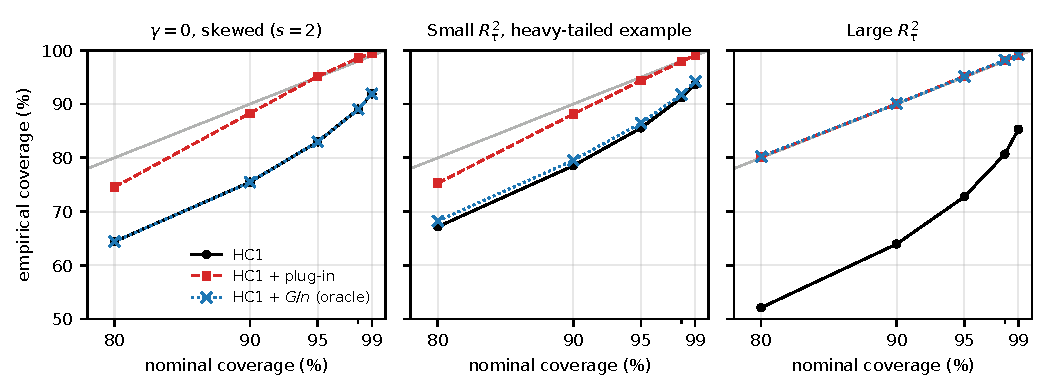
\includegraphics[width=\textwidth]{figures/calibration.pdf}
\caption{Empirical against nominal coverage for IREG with HC1, HC1 plus the plug-in correction, and HC1 plus the true $G/n$, in the three designs of Table \ref{tab:calibration}. The grey line is the diagonal. With $\gamma=0$ (left) the oracle coincides with HC1.}
\label{fig:calibration}
\end{figure}

Tables \ref{tab:correction95} and \ref{tab:calibration} and Figure \ref{fig:calibration} show three regimes. With large $R^2_\tau$ the plug-in averages \gz{corr:large_hte_n500_p5:ratio} times $G/n$, and the feasible and oracle intervals are close to nominal at every level (for example \gz{corr:large_hte_n500_p5:IREG_HC1c:0.80}\% and \gz{corr:large_hte_n500_p5:IREG_HC1o:0.80}\% at $80\%$, \gz{corr:large_hte_n500_p5:IREG_HC1c:0.99}\% and \gz{corr:large_hte_n500_p5:IREG_HC1o:0.99}\% at $99\%$), while HC1 alone undercovers at every level. The median width ratio of \gz{corr:large_hte_n500_p5:wr} is what adding a genuinely large variance component requires. In the small-$R^2_\tau$ example the oracle moves HC1 coverage by about a point, whereas the plug-in, whose average is \gz{corr:heavy_tail_example:ratio} times $G/n$, moves it by five to ten points depending on the level; with $\gamma=0$ the oracle changes nothing and the plug-in again moves coverage substantially. In these two designs the median width ratio is only \gz{corr:heavy_tail_example:wr} and \gz{corr:lognormal_s2.0_prop:wr}: a modest typical lengthening produces large changes in coverage because the HC1 interval itself is badly miscalibrated and the lengthening is concentrated where HC1 fails. With $\gamma=0$ the median width ratio is \gz{corr:lognormal_s2.0_prop:wr_miss} in replications where the HC1 interval misses and \gz{corr:lognormal_s2.0_prop:wr_cover} where it covers, whereas with large $R^2_\tau$ the lengthening is nearly uniform (\gz{corr:large_hte_n500_p5:wr_miss} and \gz{corr:large_hte_n500_p5:wr_cover}), as expected when a genuine variance component is added. Width alone therefore does not establish that an interval is valid or invalid. Across nominal levels the plug-in interval is miscalibrated in these two designs: it undercovers at $80\%$ (\gz{corr:heavy_tail_example:IREG_HC1c:0.80}\% and \gz{corr:lognormal_s2.0_prop:IREG_HC1c:0.80}\%) and slightly overcovers at $99\%$ (\gz{corr:heavy_tail_example:IREG_HC1c:0.99}\% and \gz{corr:lognormal_s2.0_prop:IREG_HC1c:0.99}\%), so its agreement with nominal at $95\%$ is a crossing point rather than evidence of a calibrated procedure; REG+HC1 shows a milder crossing in the $\gamma=0$ design (Table \ref{tab:calibration}). Here HC3 by itself is within about a point of nominal at every level, and combined with HC3 the plug-in overcovers at every level (\gz{corr:lognormal_s2.0_prop:IREG_HC3c:0.80}\% at $80\%$ with $\gamma=0$). Because $G=0$ in the last design, all of its effect there comes from the upward bias of the plug-in described in Section \ref{sec:estimand}, not from the estimand-level component. Results at $95\%$ for the 20 designs of this paper and 19 supplementary designs are in \texttt{results/correction\char`\_summary.csv}.


\section{Supplementary results for Section \ref{sec:feasible}}
\label{sec:supp-inference}

\subsection{Further designs with \texorpdfstring{$\gamma=0$}{gamma=0}}

The designs of Table \ref{tab:gamma0-other} vary the misspecification, the sample size and the number of covariates, with $Y_i(0) = 0.9\sum_{j} X_{ij} + g(X_i) + \sigma(X_i)u_i$ and $Y_i(1)=Y_i(0)+1$; with $p=5$, $X_{i1}$ is lognormal, $X_{i2},\ldots,X_{i5}\sim N(0,1)$ and $\sigma = 1+X_{i1}$. They use $20{,}000$ replications ($10{,}000$ at $n=2{,}000$ and $4{,}000$ at $n=8{,}000$), so Monte Carlo standard errors are at most \gz{mcse:maxall} percentage points. With Gaussian covariates, quadratic misspecification is harmless; with a skewed covariate, a misspecification that grows in the tail produces undercoverage even with homoskedastic noise (\gz{lognormal_s1.0_quadstd:IREG_HC1:all}\% for IREG+HC1). In the base design with $s=1.2$, the undercoverage shrinks as $n$ grows, from \gz{lognormal_s1.2_prop_n200:IREG_HC1:all}\% at $n=200$ to \gz{lognormal_s1.2_prop_n2000:IREG_HC1:all}\% at $n=2{,}000$ and \gz{lognormal_s1.2_prop_n8000:IREG_HC1:all}\% at $n=8{,}000$, and it persists with $p=5$.

\begin{table}[htbp]
\centering
\caption{Coverage (\%) of nominal $95\%$ intervals when $\gamma=0$ in further designs. Unless stated, $p=1$ and $X\sim\mathrm{LogNormal}(0,s^2)$; $Z$ is the standardized covariate.}
\label{tab:gamma0-other}
\small
\setlength{\tabcolsep}{4pt}
\begin{tabular}{lrr|cc|cc}
\toprule
& & & \multicolumn{2}{c|}{\textbf{IREG}} & \multicolumn{2}{c}{\textbf{REG}} \\
Design & $n$ & Reps & HC1 & HC3 & HC1 & HC3 \\
\midrule
\tablebody{tables/gamma0_other_body.tex}
\bottomrule
\end{tabular}
\end{table}


\subsection{Sampling variability and the second-order prediction}

\paragraph{Variability or standard error?} Coverage alone does not say whether IREG is more variable or only has a poorer standard error; Table \ref{tab:sampling} reports both. At $s=2$, the Monte Carlo standard deviation of $\htau_\IREG$ is \gz{samp:s2.0:sdI} against \gz{samp:s2.0:sdR} for $\htau_\REG$, an MSE ratio of \gz{samp:s2.0:mseratio}, while their median HC1 standard errors are almost equal (\gz{samp:s2.0:seI} and \gz{samp:s2.0:seR}): in this design IREG is genuinely more variable, and HC1 does not register the difference. Because both sampling distributions are heavy-tailed, the Monte Carlo standard deviations exceed the median standard errors even for REG, whose coverage is close to nominal, so the informative comparison is between the two estimators.

\paragraph{Connection with Section \ref{sec:asymptotics}.} The same covariate-tail features that enter the second-order MSE coefficient are also associated with more severe within-arm leverage and HC1 undercoverage in our simulations. In the designs of this section $\gamma=0$, so every term of $D_p$ that involves $\gamma$ vanishes, including the kurtosis terms; with one covariate and well-specified, shared residuals, only the product of the covariate's skewness and the heteroskedasticity moment $\EEE[Z\varepsilon^2]$ remains, and it is positive, favoring REG. Table \ref{tab:sampling} compares the implied prediction $1+\Delta/n$ with the simulated MSE ratio in the same designs: they agree closely for $s\le0.8$ (\gz{samp:s0.8:pred} predicted against \gz{samp:s0.8:mseratio} simulated at $s=0.8$), the simulated ratio exceeds one in every design, as predicted, and from $s=1$ onward the prediction exceeds the simulated ratio by a growing margin, for the reasons discussed in Appendix \ref{sec:validity}. 
\begin{table}[htbp]
\centering
\caption{Monte Carlo standard deviation and MSE of $\htau_\IREG$ and $\htau_\REG$ against their median HC1 and HC3 standard errors, in the designs of Table \ref{tab:null-main}; $\sqrt{V^*/n}$ is the common first-order standard deviation of the two estimators and $1+\Delta/n$ the second-order prediction of Theorem \ref{theo:deficiency}; Monte Carlo standard errors of the simulated MSE ratio are in parentheses, in units of the last digit.}
\label{tab:sampling}
\small
\setlength{\tabcolsep}{4pt}
\begin{tabular}{r|ccc|cc|ccc}
\toprule
& \multicolumn{3}{c|}{Standard deviation} & \multicolumn{2}{c|}{MSE ratio IREG/REG} & \multicolumn{3}{c}{Median standard error} \\
$s$ & IREG & REG & $\sqrt{V^*/n}$ & simulated & $1+\Delta/n$ & IREG HC1 & REG HC1 & IREG HC3 \\
\midrule
\tablebody{tables/sampling_body.tex}
\bottomrule
\end{tabular}
\end{table}



\subsection{Scale versus shape}

\paragraph{Scale or shape.} Table \ref{tab:scale} examines the $s=2$ design more closely. If the studentized statistic $T=(\htau-\tau)/\widehat{\mathrm{SE}}$ behaved like a scaled $t$ variable, $T\approx c\,t_{n-k}$, a single scale $c$ read off the $95\%$ coverage would predict coverage at every level. For IREG+HC1, $c=\gz{diag:scale:IREG_HC1}$, and the prediction is within \gz{diag:scale:IREG_HC1:maxdev} points of the observed coverage at every level from $80\%$ to $99\%$: HC1's failure in this design is primarily an understatement of the variance scale. The ratio of the empirical $|T|$ quantile to the $t$ quantile nevertheless rises from \gz{diag:scale:IREG_HC1:0.80:qratio} at $80\%$ to \gz{diag:scale:IREG_HC1:0.99:qratio} at $99\%$, so the tails of $T$ are also heavier than those of a scaled $t$. REG+HC1 shows a milder form of the same crossing pattern in this design: it covers \gz{diag:scale:REG_HC1:0.80:obs}\% at $80\%$ and \gz{diag:scale:REG_HC1:0.99:obs}\% at $99\%$, with the $|T|$ quantile ratio falling from \gz{diag:scale:REG_HC1:0.80:qratio} to \gz{diag:scale:REG_HC1:0.99:qratio}, so its near-nominal coverage at $95\%$ is also partly a crossing point; at $80\%$ IREG+HC3 (\gz{corr:lognormal_s2.0_prop:IREG_HC3:0.80}\%) is closer to nominal.


\begin{table}[htbp]
\centering
\caption{Scale versus shape of the studentized statistic for IREG and REG in the $\gamma=0$, $s=2$ design of Table \ref{tab:null-main}. The implied scale $c$ solves $2F_{t}(q_{0.975}/c)-1=$ observed $95\%$ coverage; ``predicted'' is $2F_t(q/c)-1$ at each level; the last row of each block divides the empirical quantile of $|T|$ by the corresponding $t$ quantile.}
\label{tab:scale}
\small
\begin{tabular}{lccccc}
\toprule
& $80\%$ & $90\%$ & $95\%$ & $98\%$ & $99\%$ \\
\midrule
\tablebody{tables/scale_body.tex}
\bottomrule
\end{tabular}
\end{table}


\subsection{HC3 and the HC3/HC1 ratio}

HC3 largely removes the scale error. In the $s=2$ design its implied scale is \gz{diag:scale:IREG_HC3} (Table \ref{tab:scale}), and the $|T|$ quantile ratio is \gz{diag:scale:IREG_HC3:0.80:qratio} at $80\%$, rising to \gz{diag:scale:IREG_HC3:0.99:qratio} at $99\%$. The remaining deviations are consistent with higher-order distortion of the studentized statistic beyond a simple scale error, which a different leverage adjustment of the variance need not remove. Table \ref{tab:gamma0-width} shows what the adjustment costs. Along the skewness sweep, the median ratio of the HC3 to the HC1 standard error of $\htau_\IREG$ rises from \gz{diag:s0.6:seratio:IREG:median} at $s=0.6$ to \gz{diag:s2.0:seratio:IREG:median} at $s=2$, with a $90$th percentile of \gz{diag:s2.0:seratio:IREG:p90}; for REG the corresponding values at $s=2$ are \gz{diag:s2.0:seratio:REG:median} and \gz{diag:s2.0:seratio:REG:p90}. The median HC1 widths of IREG and REG are nearly equal throughout (\gz{diag:s2.0:width:IREG_HC1} and \gz{diag:s2.0:width:REG_HC1} at $s=2$), so IREG+HC1's undercoverage is not accompanied by narrower typical intervals, and the gap between the median and the $90$th percentile of the HC3/HC1 ratio shows that HC3's adjustment is concentrated in a minority of replications. HC3 remains below nominal under very heavy-tailed covariates (Table \ref{tab:null-main}, $s \geq 1.8$).


\begin{table}[htbp]
\centering
\caption{Median width of nominal $95\%$ intervals and the ratio $\mathrm{SE}_{\mathrm{HC3}}(\htau)/\mathrm{SE}_{\mathrm{HC1}}(\htau)$ (median and $90$th percentile over replications) in the designs of Table \ref{tab:null-main}.}
\label{tab:gamma0-width}
\small
\begin{tabular}{r|cccc|cc|cc}
\toprule
& \multicolumn{4}{c|}{Median width} & \multicolumn{2}{c|}{IREG HC3/HC1} & \multicolumn{2}{c}{REG HC3/HC1} \\
$s$ & IREG HC1 & IREG HC3 & REG HC1 & REG HC3 & median & p90 & median & p90 \\
\midrule
\tablebody{tables/gamma0_width_body.tex}
\bottomrule
\end{tabular}
\end{table}


\subsection{Covariate representation}

The covariate representation matters accordingly. On the same $s=2$ datasets, adjusting for $\log(1+X)$ instead of $X$ lowers the median of the largest IREG leverage from \gz{tr:X:lev} to \gz{tr:log1pX:lev}, and IREG+HC1 then covers \gz{tr:log1pX:IREG_HC1:cov}\% instead of \gz{tr:X:IREG_HC1:cov}\%; but the median interval widens from \gz{tr:X:IREG_HC1:width} to \gz{tr:log1pX:IREG_HC1:width}, because the outcome is linear in $X$ in this design. The check ties the extreme undercoverage to the tail of the raw covariate; it does not show that transformation is generally preferable.



\subsection{Leverage one and software}

\paragraph{Leverage one.} An observation with an extreme covariate value can carry a large share of the variance of $\htau_\IREG$. When a treatment arm contains exactly one such observation, it has leverage one in that arm's fit and is fitted exactly, so its residual is zero. A residual-based variance estimator then has no information about the observation's contribution: HC1 counts it as zero, and HC2 and HC3 face a $0/0$ that no leverage adjustment can resolve. To isolate this we use a rare-value design: $p=1$, $n=500$, $X_{i1}=\sqrt{(1-\rho)/\rho}$ with probability $\rho=0.02$ and $-\sqrt{\rho/(1-\rho)}$ otherwise, and $\sigma = 1+|X_{i1}|$ or $\sigma=1$. An arm contains exactly one rare unit, and the other arm at least one, in \gz{rare_q0.02_prop:lev1}\% of replications (exact probability \gz{rare:theory:lev1}\%) (Table \ref{tab:gamma0-rare}; each leverage-one subset contains at least \gz{lev1:n:min} replications, so the Monte Carlo standard errors of its coverages are at most \gz{lev1:mcse:max} points). With $\sigma=1+|X_{i1}|$ the isolated unit also carries the largest residual variance, and IREG+HC1 covers \gz{rare_q0.02_prop:IREG_HC1:lev1}\% of those replications; with $\sigma=1$, IREG+HC1 covers \gz{rare_q0.02_homo:IREG_HC1:lev1}\% of those replications. In \gz{rare_q0.02_prop:rankdef}\% of replications (exact probability \gz{rare:theory:rankdef}\%) an arm contains no rare unit and the interacted design is rank-deficient; these replications are included in the ``all replications'' rows as the software reports them. REG estimates a single slope from both arms and does not create the same arm-specific leverage problem induced by the interacted specification; it stays near nominal at $95\%$ in every row of the table.

\paragraph{Software.} What HC2 and HC3 report at leverage one depends on how software evaluates the $0/0$, and packages do not treat full-leverage observations consistently \citep{Kranz2024}. Table \ref{tab:gamma0-rare} reports two versions of \texttt{estimatr}, which handle the case differently (Appendix \ref{sec:r-validation}); neither recovers the variance contribution of the isolated observation.

\begin{table}[htbp]
\centering
\caption{Coverage (\%) in the rare-value design ($\gamma=0$, $p=1$, $n=500$, $\rho=0.02$, $20{,}000$ replications). Rows: all replications as the software reports them; replications with a full-rank interacted design; and, within those, replications in which an arm contains a leverage-one unit. With $\sigma=1+|X_1|$ these are \gz{rare_q0.02_prop:rankdef}\% rank-deficient and \gz{rare_q0.02_prop:lev1}\% leverage-one replications; with $\sigma=1$, \gz{rare_q0.02_homo:rankdef}\% and \gz{rare_q0.02_homo:lev1}\%; the exact probabilities are \gz{rare:theory:rankdef}\% and \gz{rare:theory:lev1}\%. The two \texttt{estimatr} versions are applied to the same simulated datasets; they differ only in how they evaluate the $0/0$ HC2/HC3 contribution and in which collinear column they drop in rank-deficient fits. REG does not depend on the version. A replication without a finite interval counts as a non-cover.}
\label{tab:gamma0-rare}
\small
\setlength{\tabcolsep}{4pt}
\begin{tabular}{l|ccc|ccc|cc}
\toprule
& \multicolumn{3}{c|}{\textbf{IREG}, v\gz{estimatr:v1}} & \multicolumn{3}{c|}{\textbf{IREG}, v\gz{estimatr:v2}} & \multicolumn{2}{c}{\textbf{REG}} \\
& HC1 & HC2 & HC3 & HC1 & HC2 & HC3 & HC1 & HC3 \\
\midrule
\tablebody{tables/gamma0_rare_body.tex}
\bottomrule
\end{tabular}
\end{table}


\subsection{Designs of the combined battery}

The battery of Section \ref{sec:combined} reuses the designs of the correction study. \emph{Gaussian}: $X_i\sim N(0,I_5)$ (small HTE) or $N(0,\Sigma)$ with $\Sigma_{jk}=0.5^{|j-k|}$ (large HTE), homoskedastic $N(0,1)$ noise. \emph{Misspecified}: $X_i\sim N(0,\Sigma)$ as above and $Y_i(0)=0.9\sum_jX_{ij}+0.2(X_{i1}^2-1)+0.15X_{i1}X_{i2}+u_i$. \emph{Skewed} and \emph{heavy-tailed}: $X_{i1}$ is a centered $\mathrm{LogNormal}(0,s^2)$ variable with $s=1.1$ or $s=1.5$, mixed with four independent standard normal coordinates by an AR(0.35) Cholesky factor and standardized, with $\sigma(X)=1+c|X_{i1}|+0.25\|X_i\|$ and $c=0.5$ or $0.75$. \emph{Rare extreme values}: $X_{i1}$ takes the value $\sqrt{(1-\rho)/\rho}$ with probability $\rho=0.02$ and $-\sqrt{\rho/(1-\rho)}$ otherwise, the other coordinates are standard normal, and the noise is homoskedastic. In every design $Y_i(1)=Y_i(0)+1+\gamma^*X_{i1}$, with the potential outcomes sharing their noise, and $R^2_\tau$ is computed from the design ($\EEE[\varepsilon^2]$ by $10^6$ Monte Carlo draws where it has no closed form). These simulations use the NumPy implementation cross-validated against \texttt{estimatr} in Appendix \ref{sec:r-validation}; in the rare-value design it drops the contribution of a leverage-one observation to HC3, like the development version of \texttt{estimatr}.

\begin{table}[htbp]
\centering
\caption{Further intervals for the designs of Table \ref{tab:battery}: coverage (\%) of nominal $95\%$ intervals for the population ATE, and the ratio of the average plug-in term to $G/n$.}
\label{tab:battery-supp}
\small
\setlength{\tabcolsep}{4pt}
\begin{tabular}{l|cccc|c|c}
\toprule
& \multicolumn{4}{c|}{IREG} & REG & plug-in \\
Design & HC1 & HC1 + oracle & HC3 & HC3 + plug-in & HC3 & $/(G/n)$ \\
\midrule
\tablebody{tables/hte_battery_supp_body.tex}
\bottomrule
\end{tabular}
\end{table}

\end{document}
